\section{Summary}

The following tables and figures summarize the azimuthal asymmetries of charged pions, $\pi^0$ and $\eta$. 
The measured asymmetries are corrected for smearing effects, background contributions and false asymmetries according to the following formula:
\begin{equation}
A=(A_\textrm{raw,bg corrected}-A_\textrm{MC})\times f_S
\end{equation}
Here, $A_\textrm{raw,bg corrected}$ is the raw asymmetry after background correction which is described in section~\ref{sec:backgroundcorrection}.
$A_\textrm{MC}$ is the false asymmetry measured in simulation. The later are not corrected for background asymmetries, since we are only interested in the detector effects on the asymmetries.
Finally, the corrected asymmetry is corrected for smearing using the smearing correction $f_S$ as outlined in section~\ref{sec:smearingcorrection}.

These systematics are determined from simulation as described earlier in this note. Systematic uncertainties arise from the statistical uncertainties on the smearing effects, the background contribution and the false asymmetries according to the following expression:
\begin{equation}
\sqrt{ A^2*(\frac{\sigma_{f_S}}{f_S})^2+(f_S*\sigma_F)^2+(f_S*\sigma_{A_\textrm{MC}})^2}.
 \end{equation}
 Here $\sigma_F$ is the uncertainty on the fit to extract the $\pi^0$ signal. As described in section~\ref{sec:neutralmesonreconstruction}, this uncertainty accounts for the difference in extracted asymmetries if either the crystal-ball fit or the non-parametric signal fit using MC templates is used to determine the signal count rates. (The crystal-ball result is used for the asymmetry value).
 
The measured values for the Collins asymmetry show a significant increase with $z$ and $P_t$. The UL double ratio asymmetries are larger than UC and $\pi^0$ asymmetries while UC and $\pi^0$ asymmetries are similar. 
In table~\ref{tab:finalpi0zbin}~\ref{tab:finalpi0ptbin} and~\ref{tab:finaletazbin}~\ref{tab:finaletaptbin} the only different constraint for $\pi^0$ vs. $\eta$ is that the photon energy threshold for $\eta$ is higher than $\pi^0$. Section~\ref{sec:resultsfromexp} discusses the comparison between $\eta$ and $\pi^0$ when the same photon energy constraint is applied and Fig.~\ref{fig:finalasymmetry1}~\ref{fig:finalasymmetry2} show the comparison after background and thrust smearing corrections. The corresponding numerical values can be found in tables~\ref{tab:finalpi0zbin}-\ref{tab:finalulucptbins}. Due to the large error bars of $\eta$ no significant difference can be obtained between $\pi^0$ and $\eta$. In the last section~\ref{sec:newbins}, new kinematic bins reveal more information about the relationship between kinematic and Collins asymmetry. 

Besides the background and thrust smearing corrections discussed in sections \ref{sec:backgroundcorrection} and \ref{sec:smearingcorrection} respectively, section~\ref{sec:charmcontribution} gives the percentage contribution of charm. With the study of Collins effect for charm in the future, charm contribution in the Collins asymmetries of $\pi^0$ and $\eta$ can be corrected. 


\begin{figure}[H]
  %\ContinuedFloat
  \centering
  \subfigure{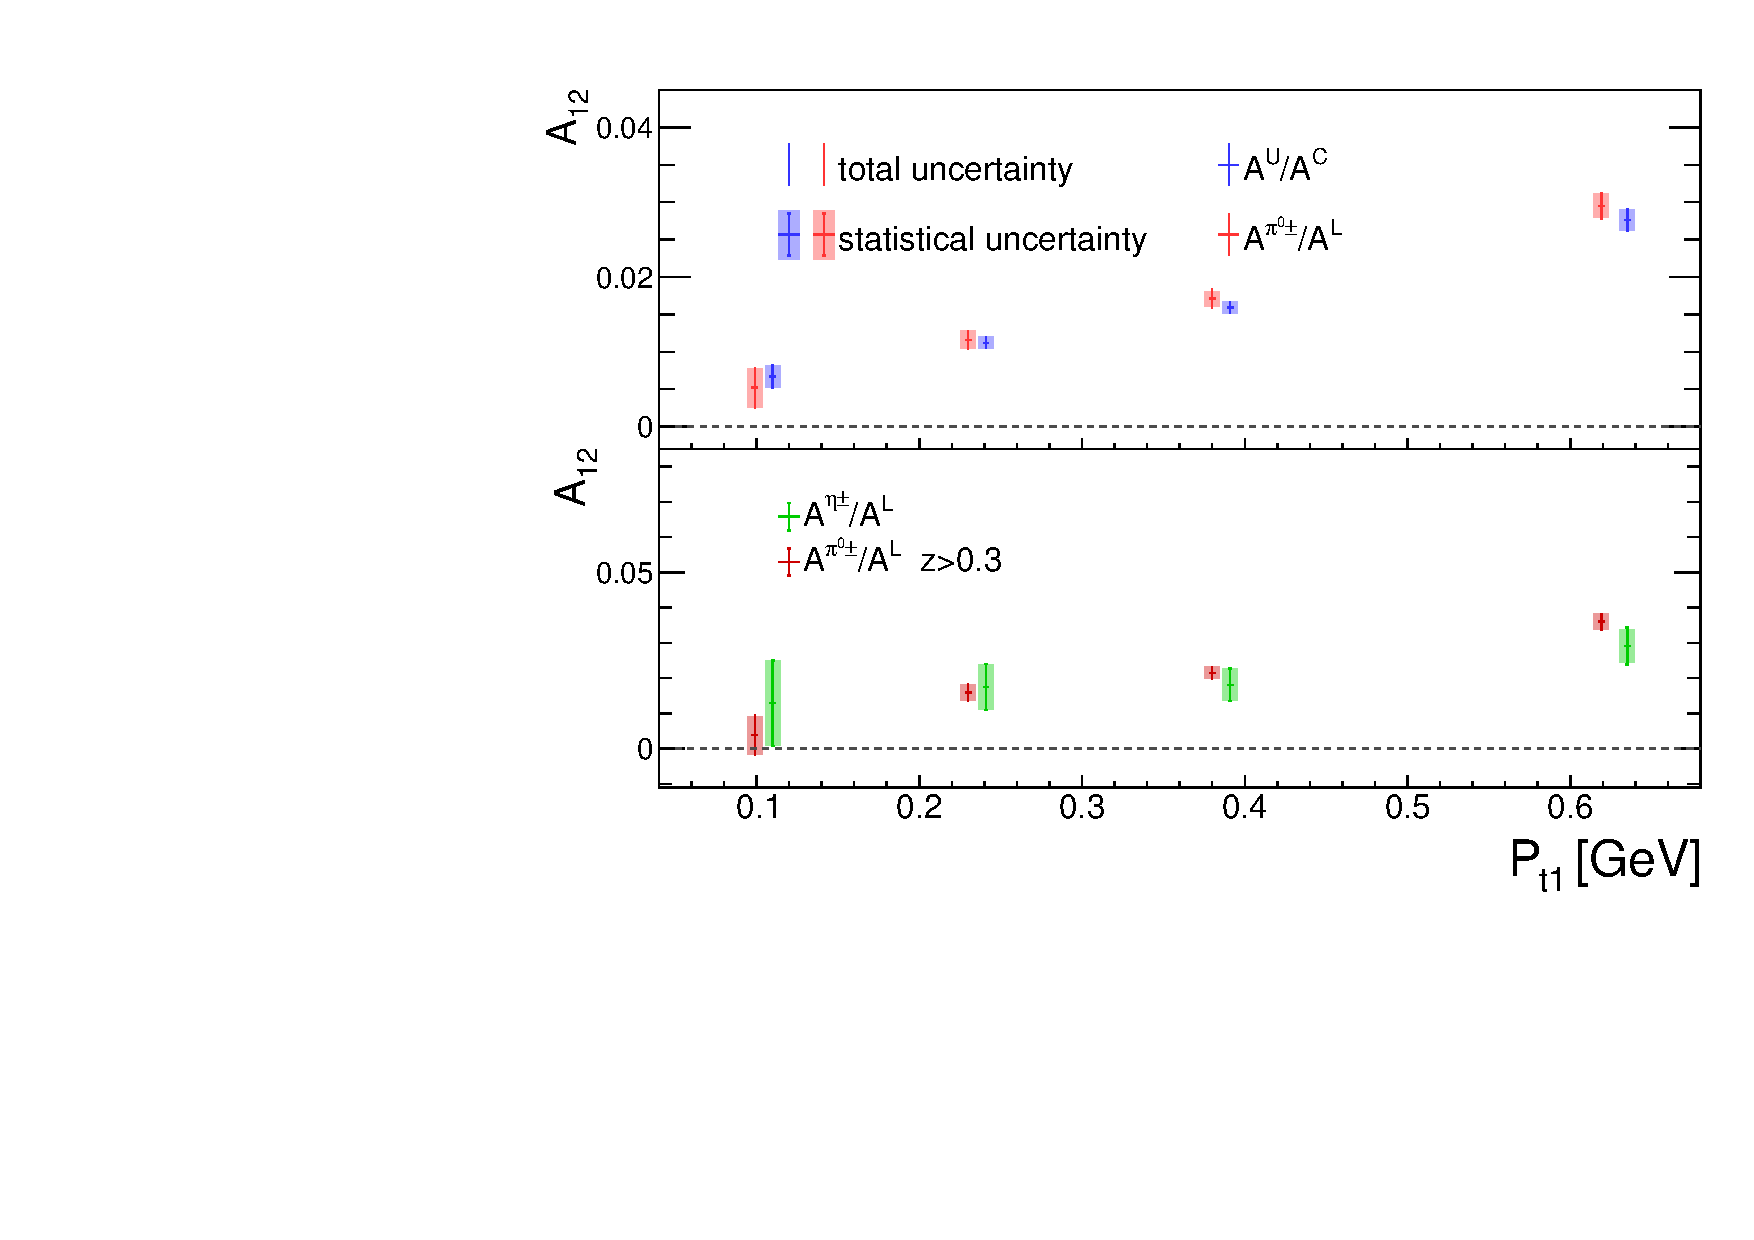
\includegraphics[width=0.45\textwidth,natwidth=200,natheight=150]{figure_asy/pi0_eta_sinpt.pdf}}
  \subfigure{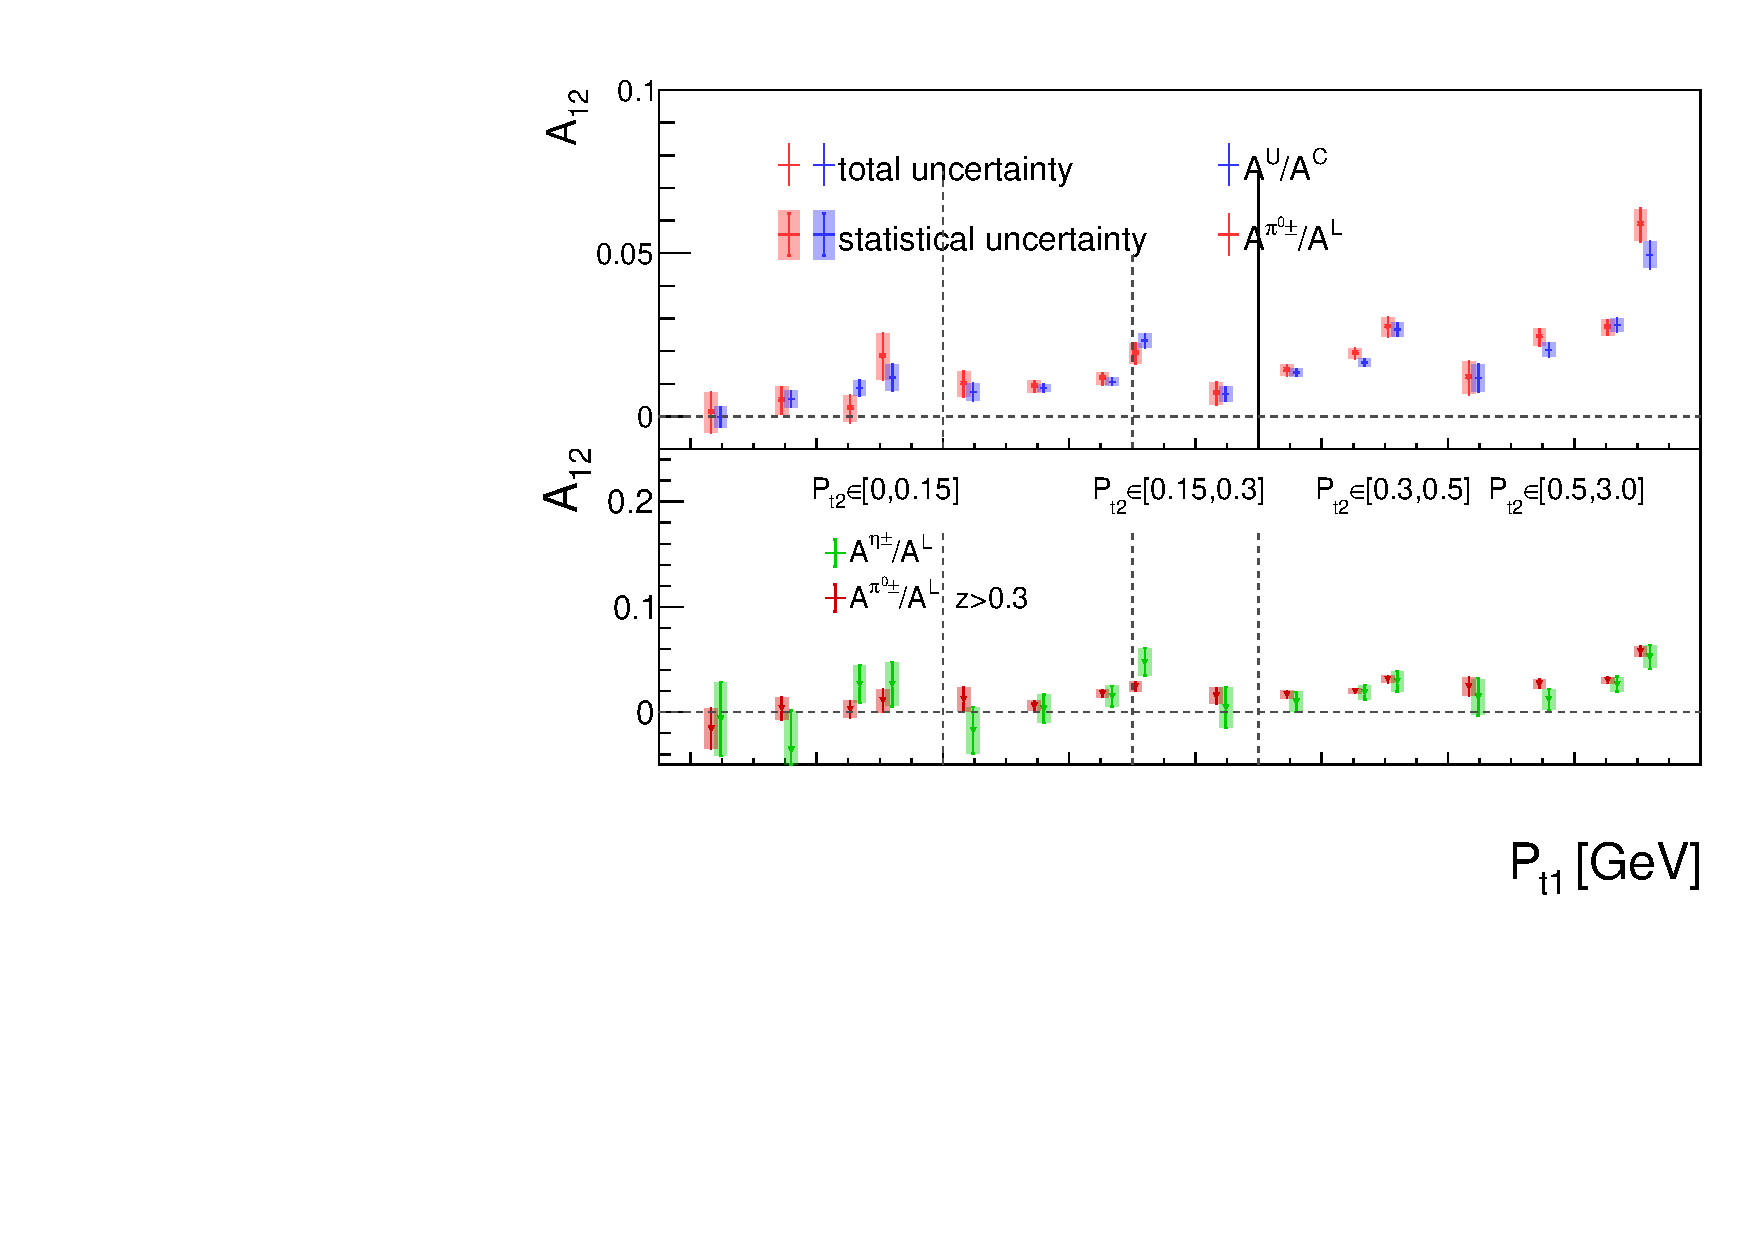
\includegraphics[width=0.45\textwidth,natwidth=200,natheight=150]{figure_asy/pi0_eta_compt16bin.pdf}}
\caption{The Collins asymmetry of $\pi^0$, UC and $\eta$ as a function of the transverse momentum $P_t$. In lower panels the photon energy and $z$ criterion applied to $\eta$ are applied on $\pi^0$. The x coordinates of $\pi^0$ are centroids of kinematic bins while the horizontal position of UC and $\eta$ points are shifted to avoid overlapping. The inner shaded regions represent the statistical uncertainties of each data point, while the outer error bars show the total uncertainties.}
\label{fig:finalasymmetry1}
\end{figure}

\begin{figure}[H]
  \centering     
  \subfigure{\label{fig:sinz}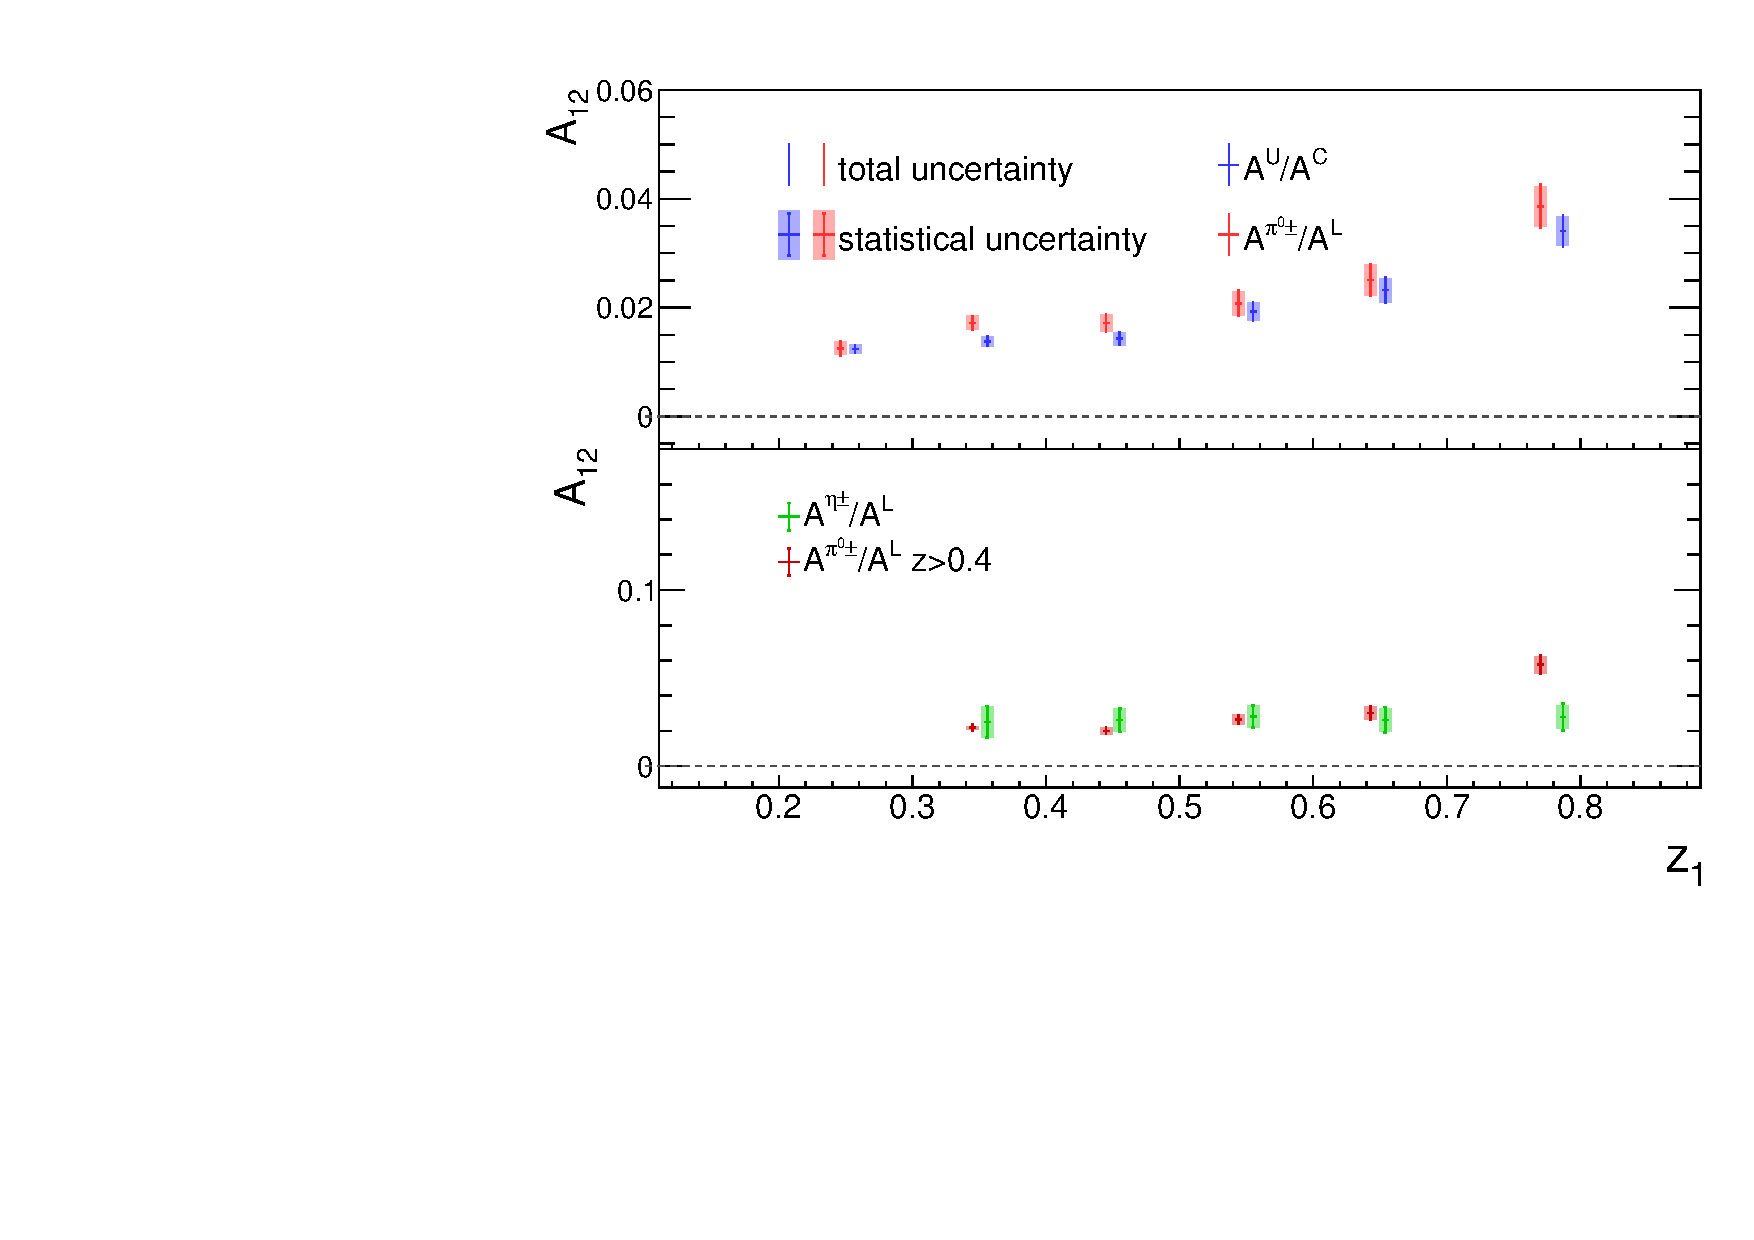
\includegraphics[width=0.45\textwidth,natwidth=200,natheight=150]{figure_asy/pi0_eta_sinz.pdf}}
  \subfigure{\label{fig:comz}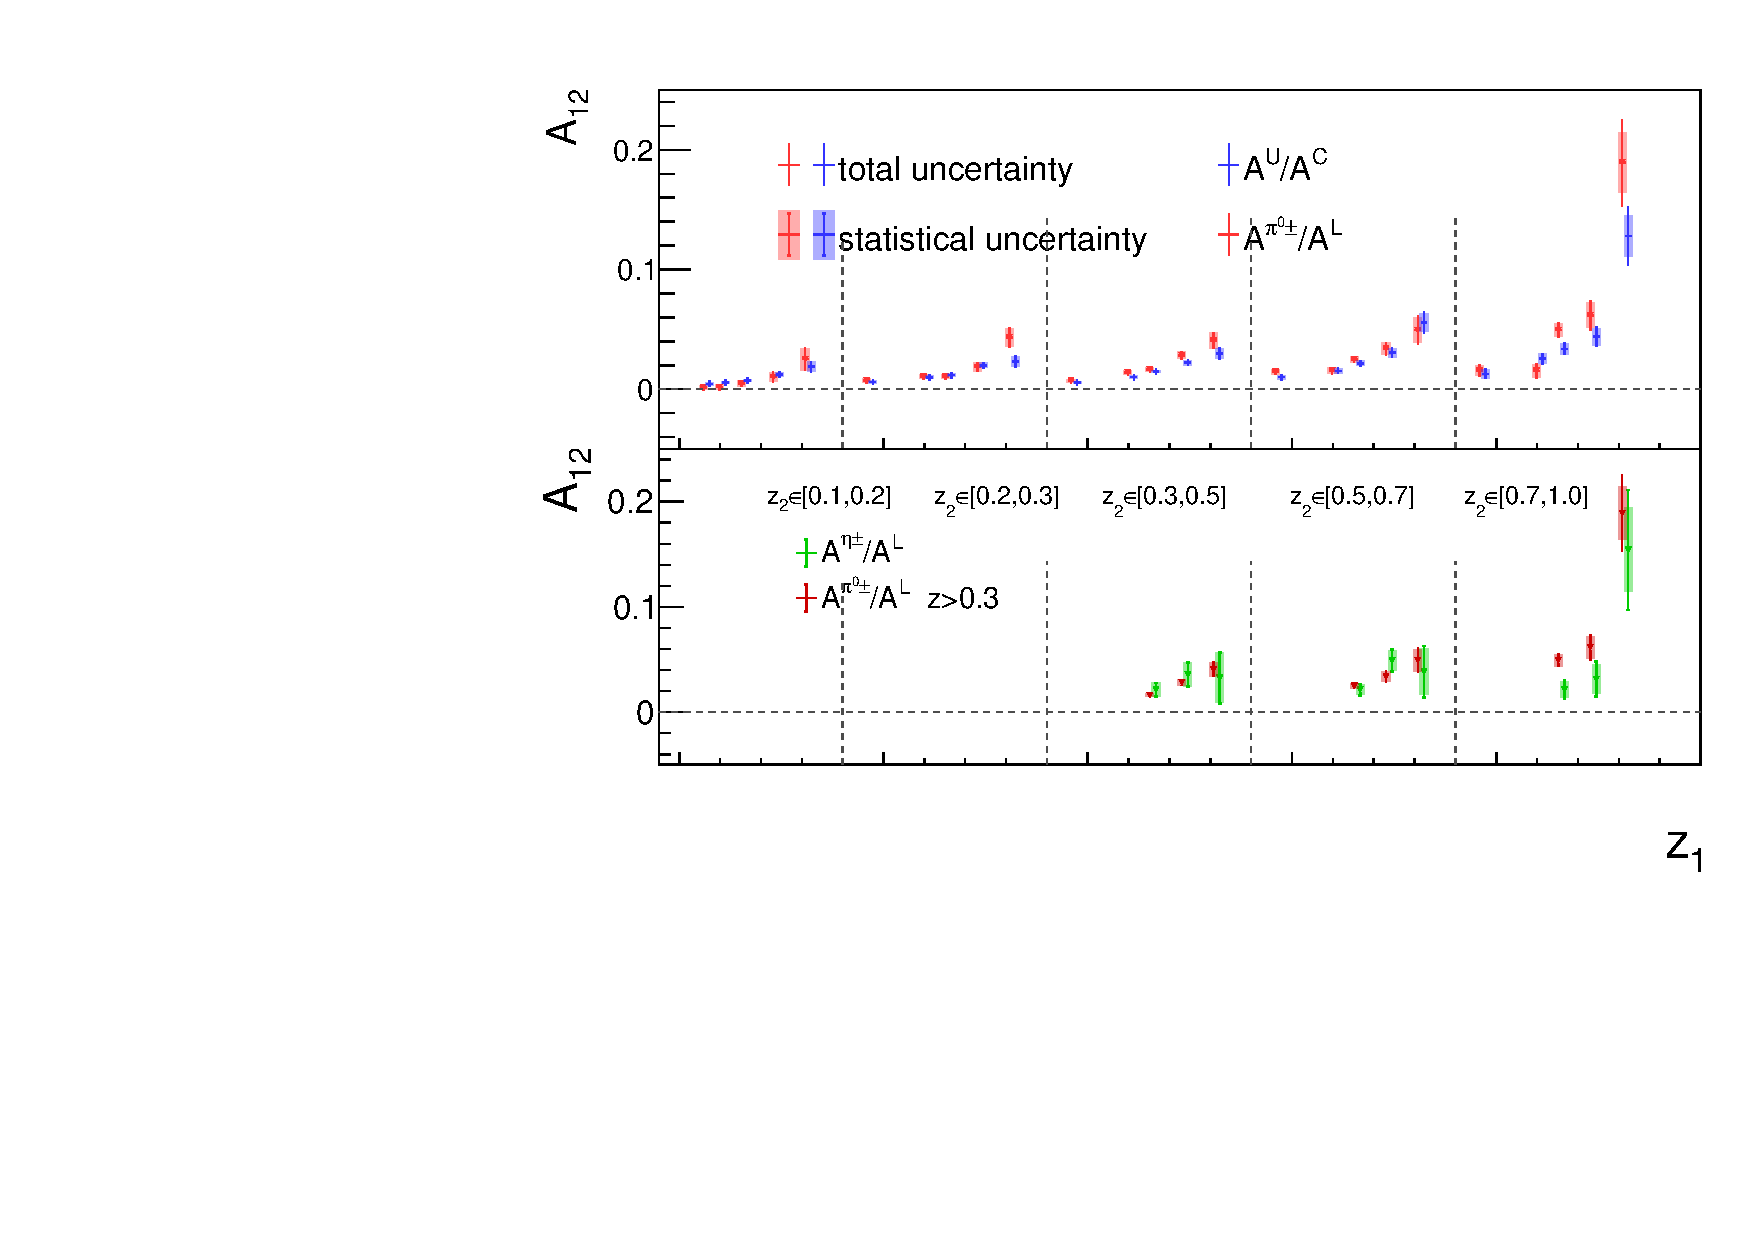
\includegraphics[width=0.45\textwidth,natwidth=200,natheight=150]{figure_asy/pi0_eta_comz25bin.pdf}}
\caption{The Collins asymmetry $A_{12}$ of $\pi^0$, UC and $\eta$ as a function of the fractional energy $z$. In lower panels the photon energy and $z$ criterion applied to $\eta$ are applied on $\pi^0$. The x coordinates of $\pi^0$ are the centroids of kinematic bins while the horizontal position of UC and $\eta$ points are shifted to avoid overlapping. The inner shaded regions represent the statistical uncertainties of each data point, while the outer error bars show the total uncertainties.}
\label{fig:finalasymmetry2}
\end{figure}

\begin{figure}[H]
  \centering     
  \subfigure{\label{fig:comz2}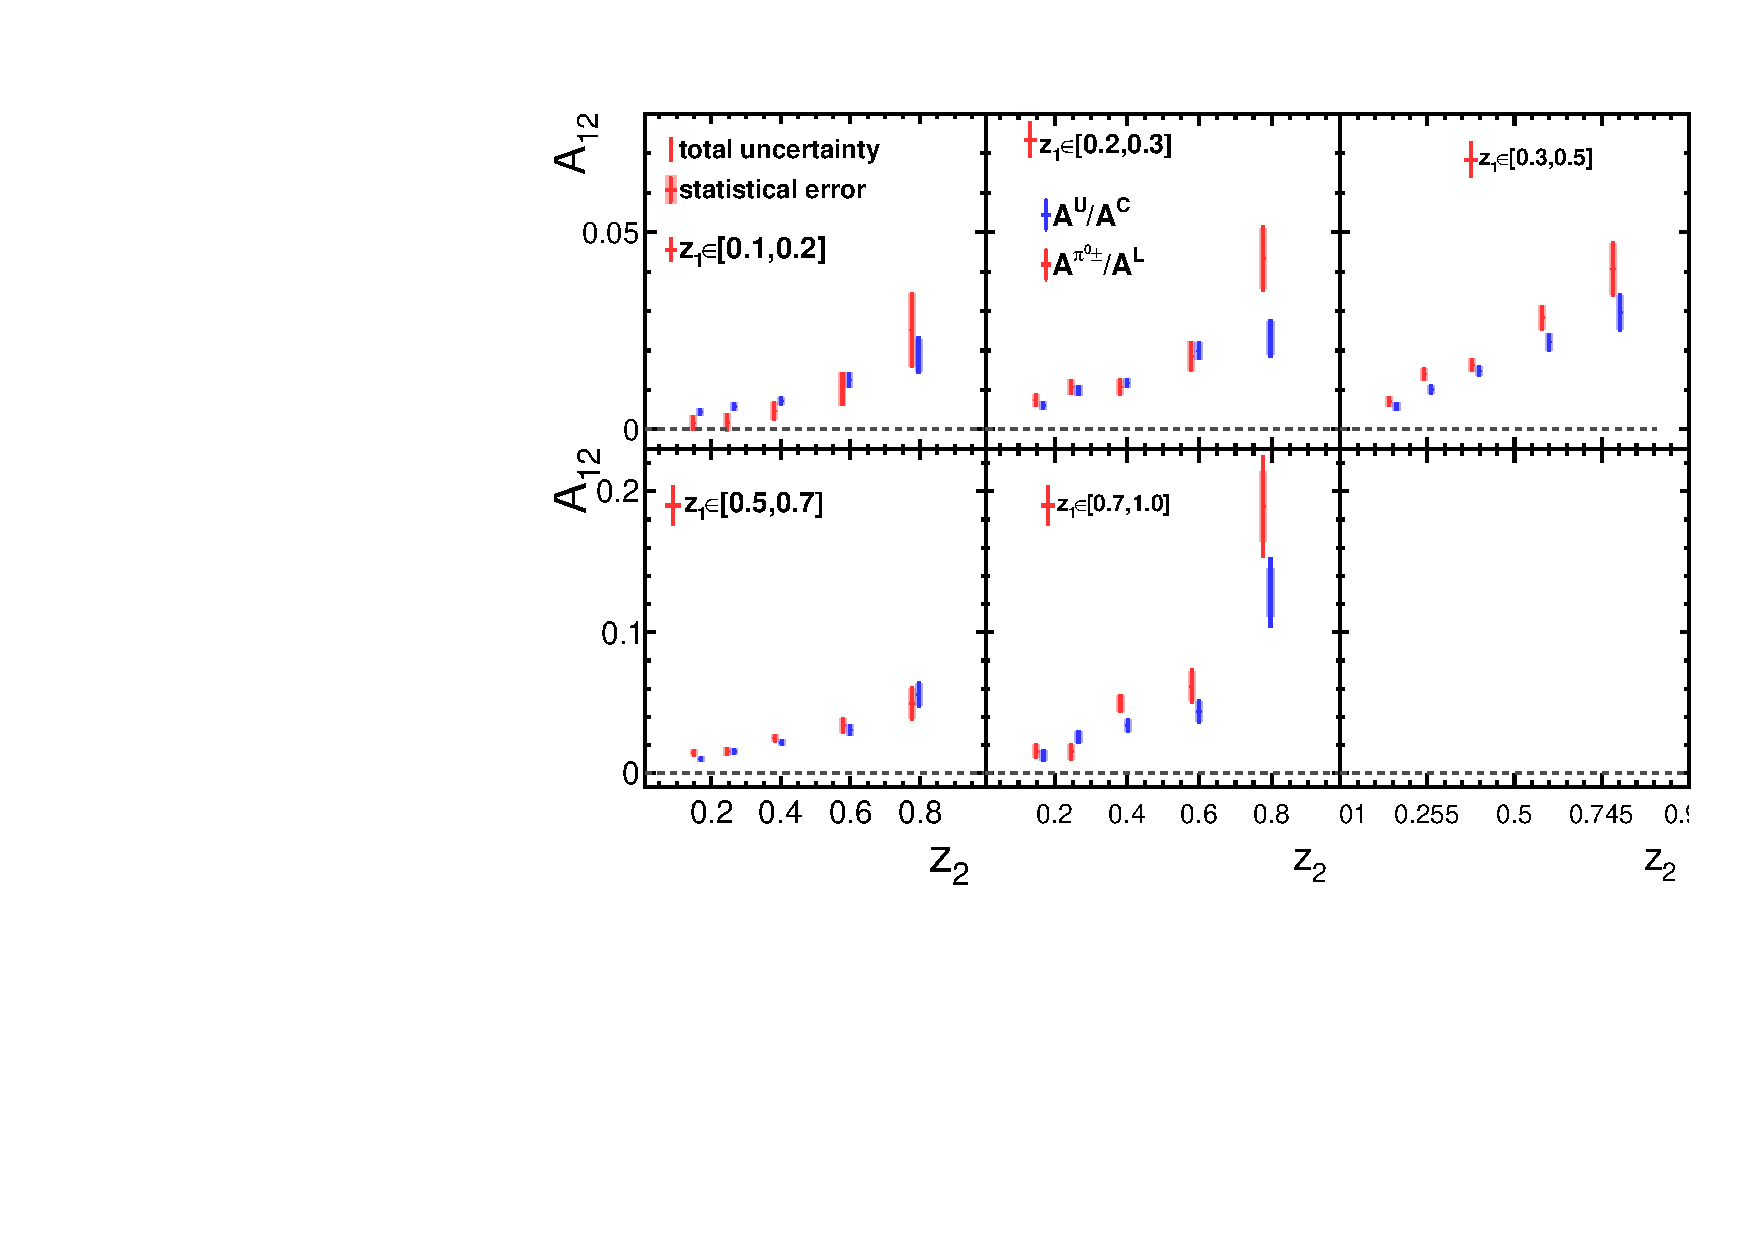
\includegraphics[width=0.45\textwidth,natwidth=200,natheight=150]{figure_asy/pi0_uc_comz_bin.pdf}}
  \subfigure{\label{fig:compt2}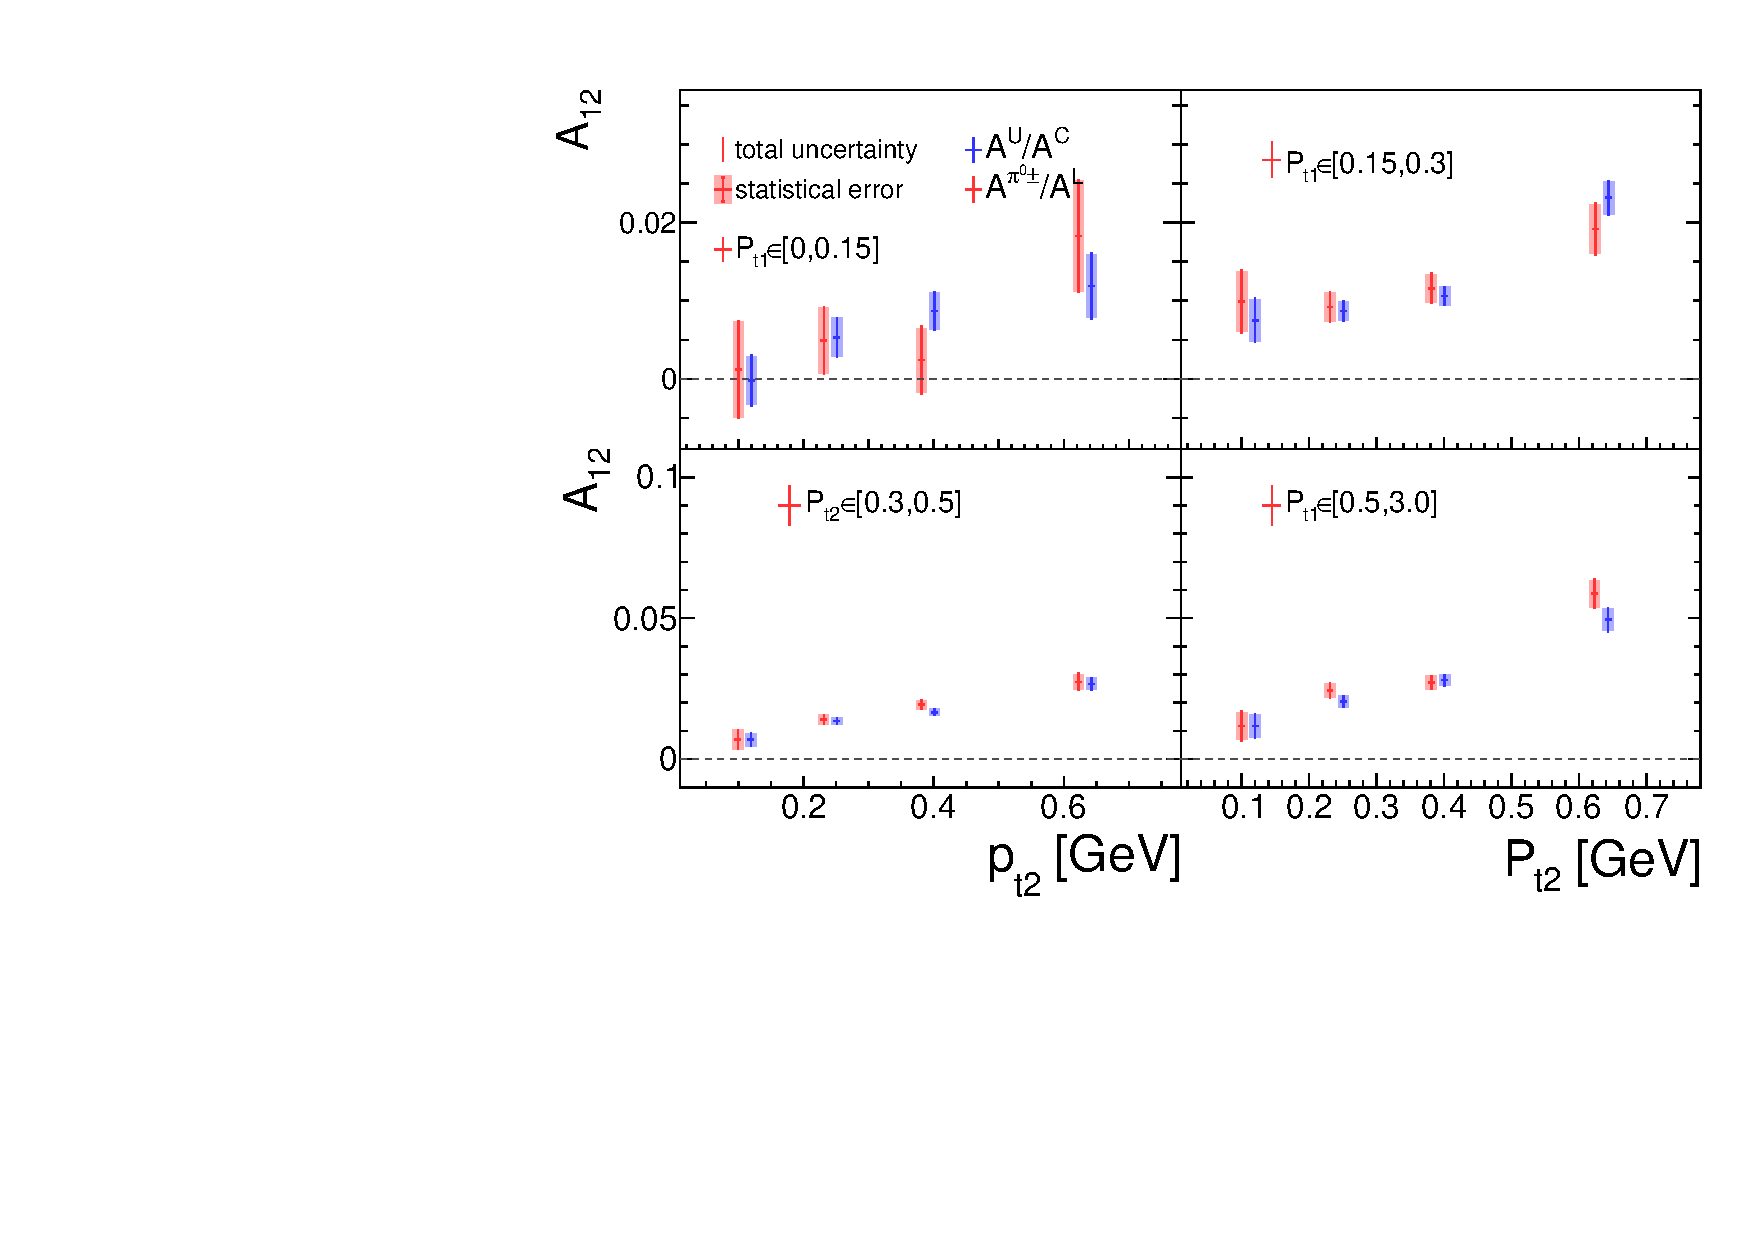
\includegraphics[width=0.45\textwidth,natwidth=200,natheight=150]{figure_asy/pi0_uc_compt_bin.pdf}}
  \subfigure{\label{fig:comz3}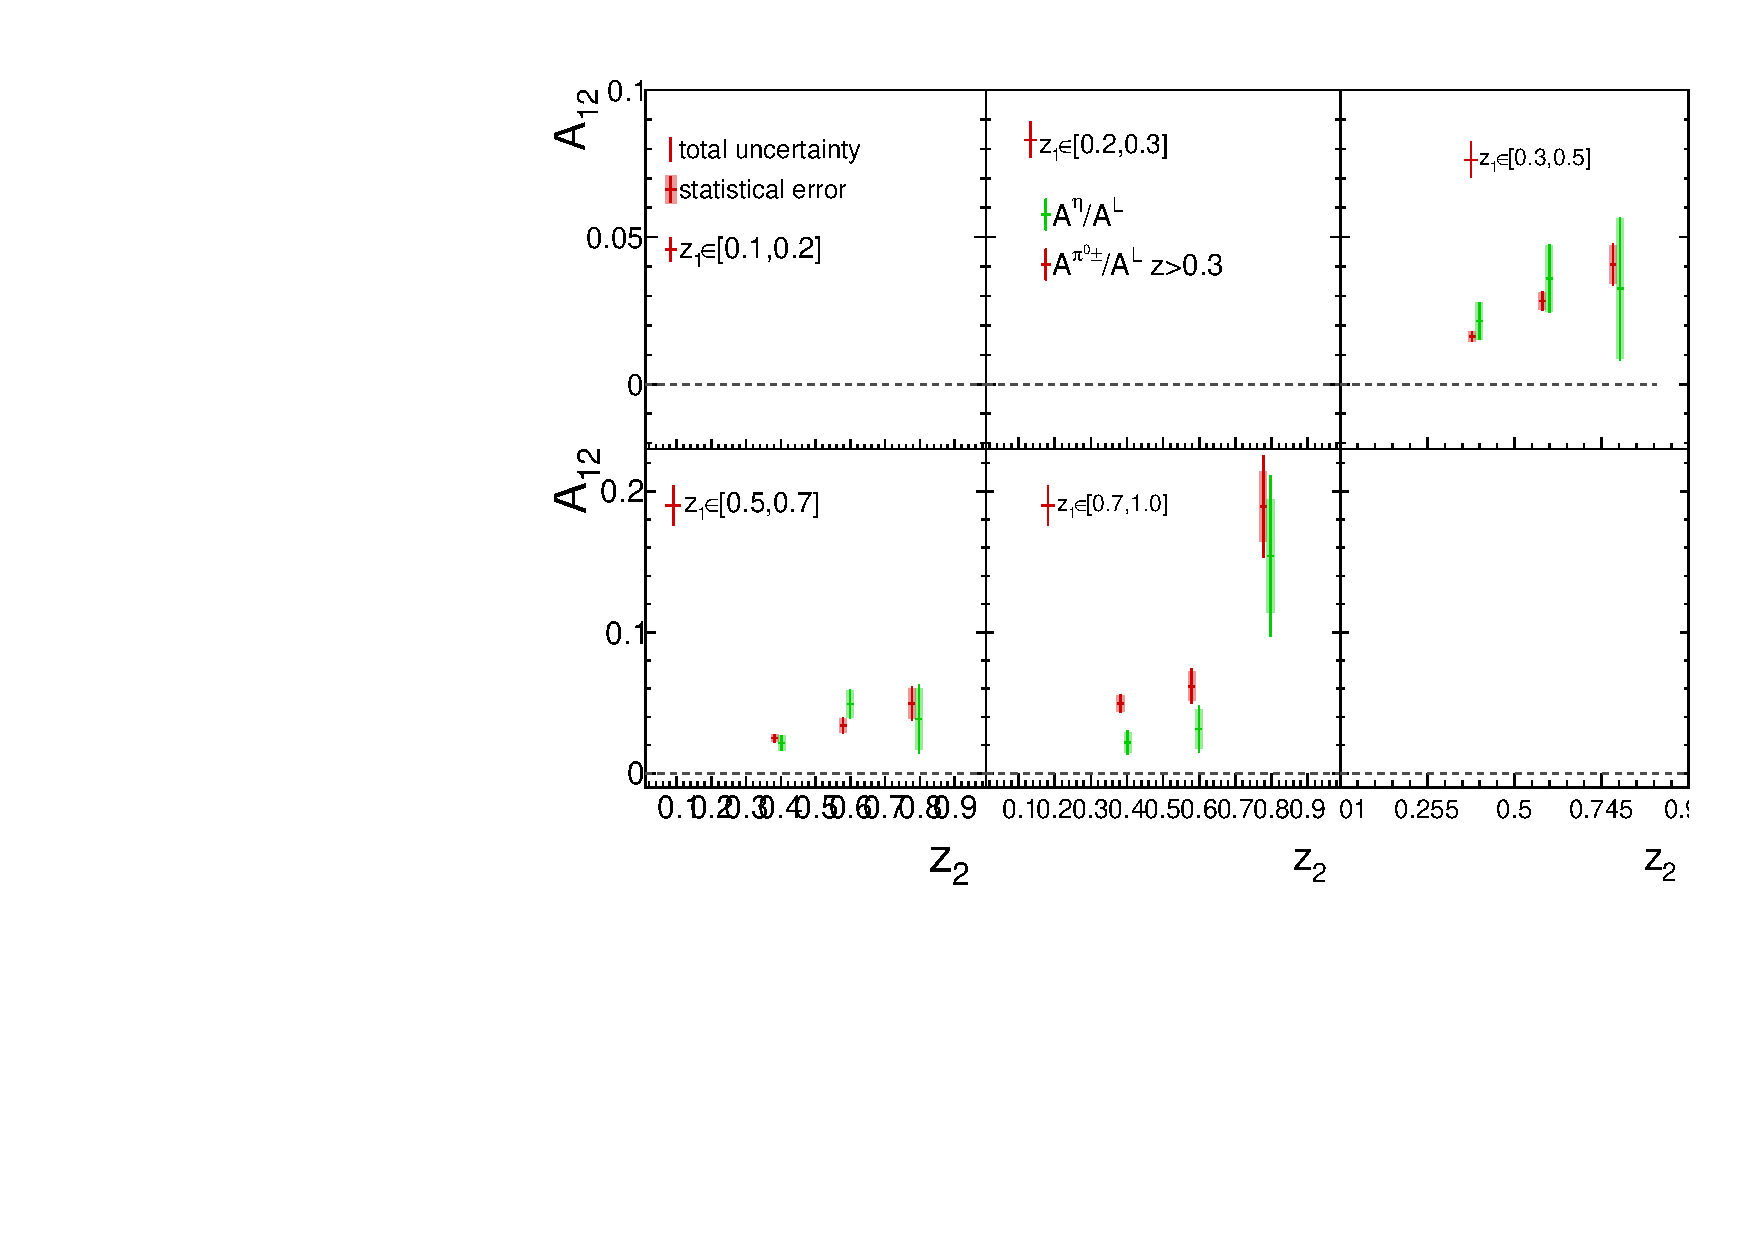
\includegraphics[width=0.45\textwidth,natwidth=200,natheight=150]{figure_asy/eta_pi0_comz_bin.pdf}}
  \subfigure{\label{fig:compt3}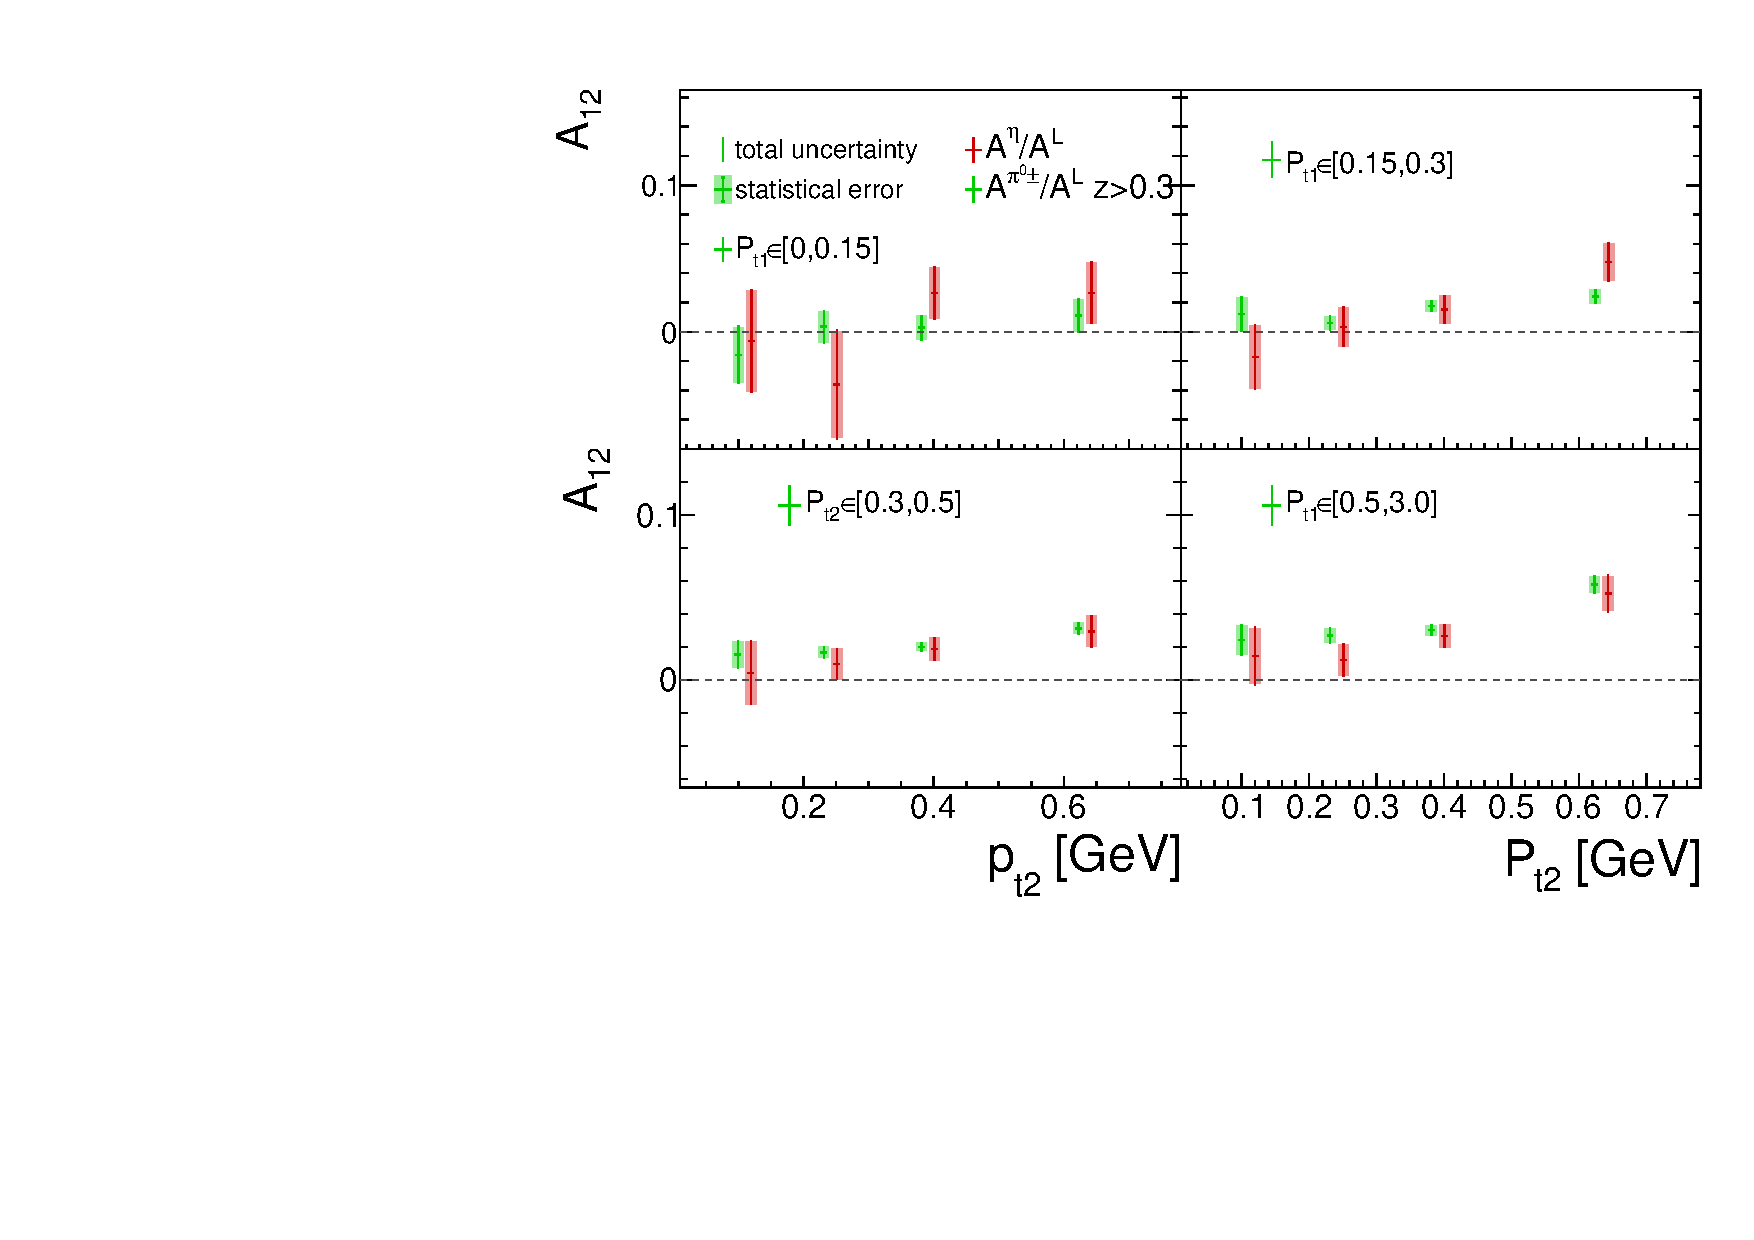
\includegraphics[width=0.45\textwidth,natwidth=200,natheight=150]{figure_asy/eta_pi0_compt_bin.pdf}}
\caption{Another illustration of asymmetries in $(z_1,z_2)$ and $(P_{t1},P_{t2})$ bins. The Collins asymmetry $A_{12}$ of $\pi^0$, UC and $\eta$ as a function of the fractional energy $z$. In lower panels the photon energy and $z$ criterion applied to $\eta$ are applied on $\pi^0$. The x coordinates are the centroids of kinematic bins while the horizontal position of UC and $\eta$ points are shifted to avoid overlapping. The inner shaded regions represent the statistical uncertainties of each data point, while the outer error bars show the total uncertainties.}
\label{fig:finalasymmetry4}
\end{figure}

\begin{figure}[H]
  \centering     
  \subfigure{\label{fig:16bin2}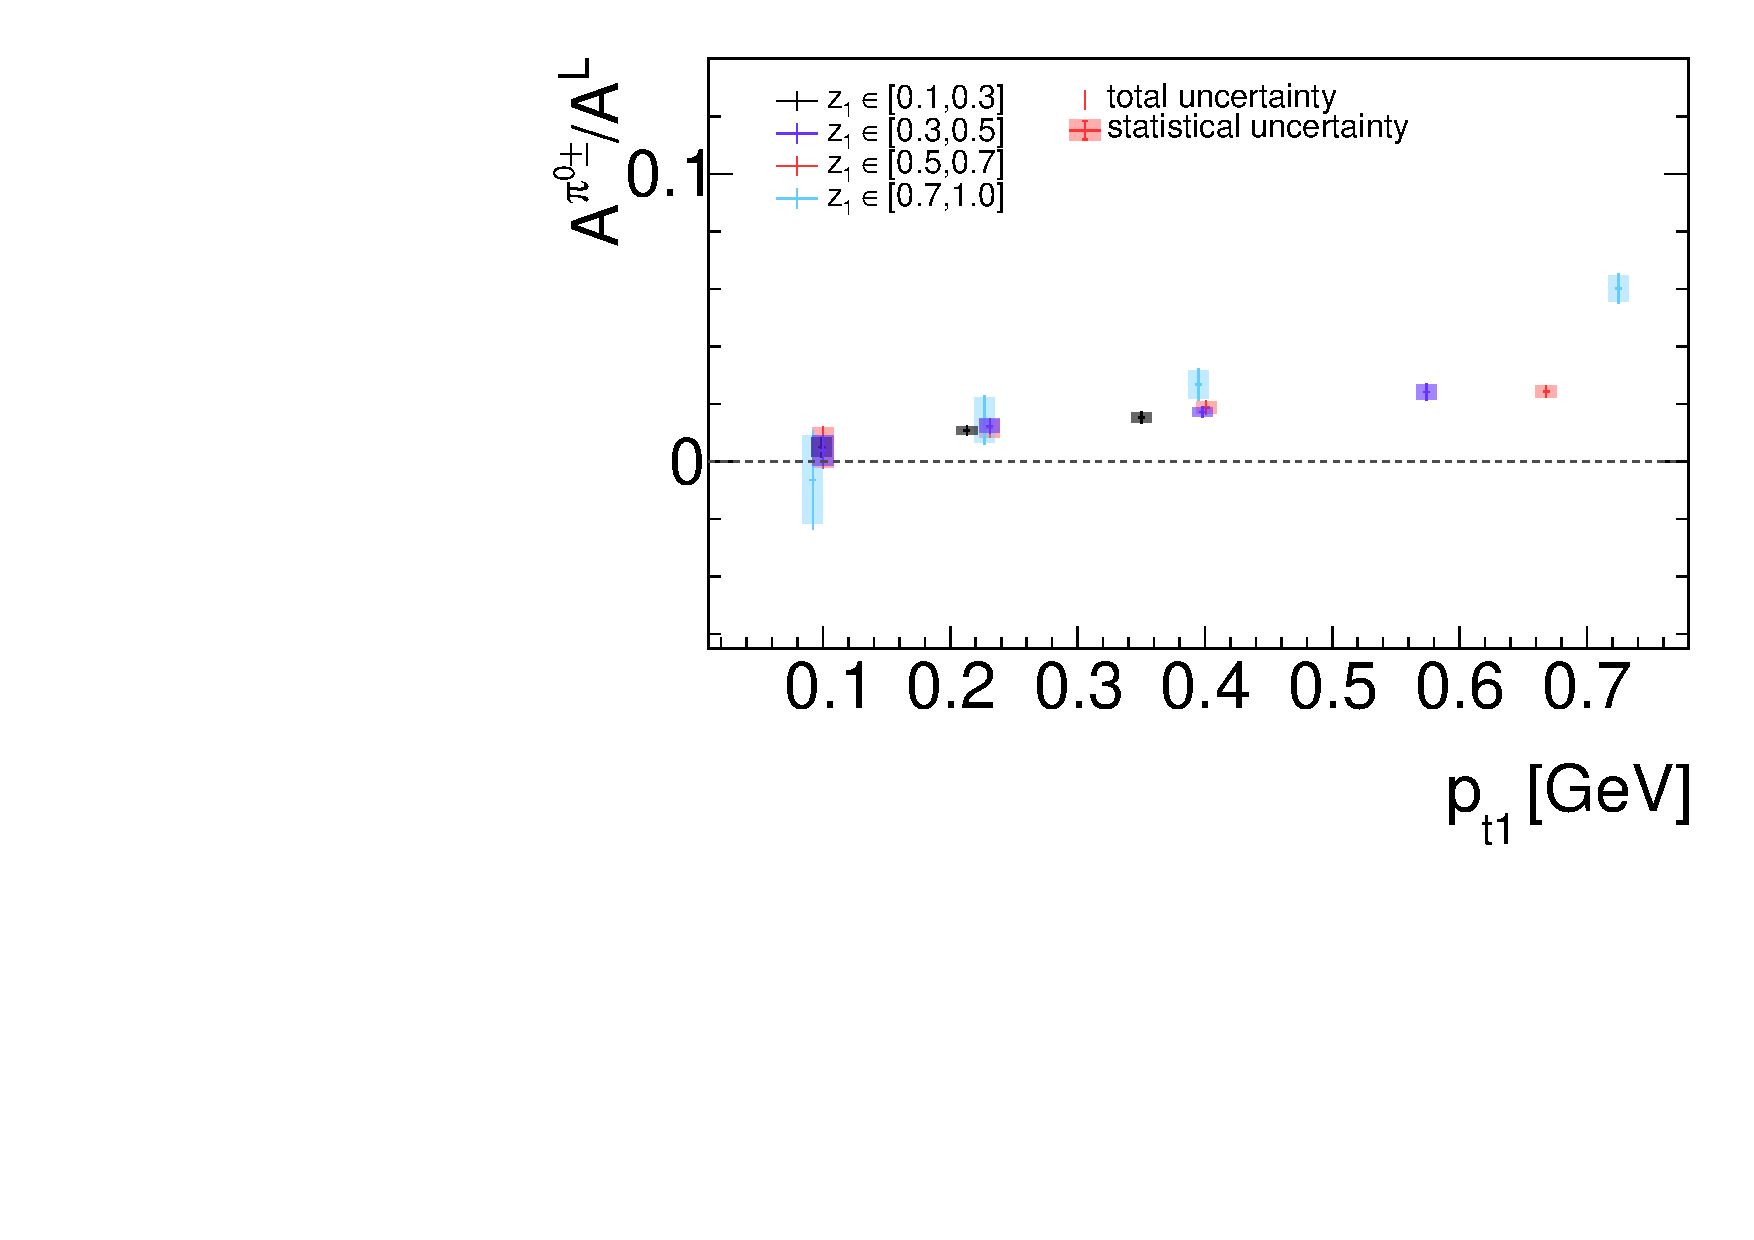
\includegraphics[width=0.45\textwidth,natwidth=200,natheight=150]{figure_asy/pi0_16bin_2.pdf}}
  \subfigure{\label{fig:16bin3}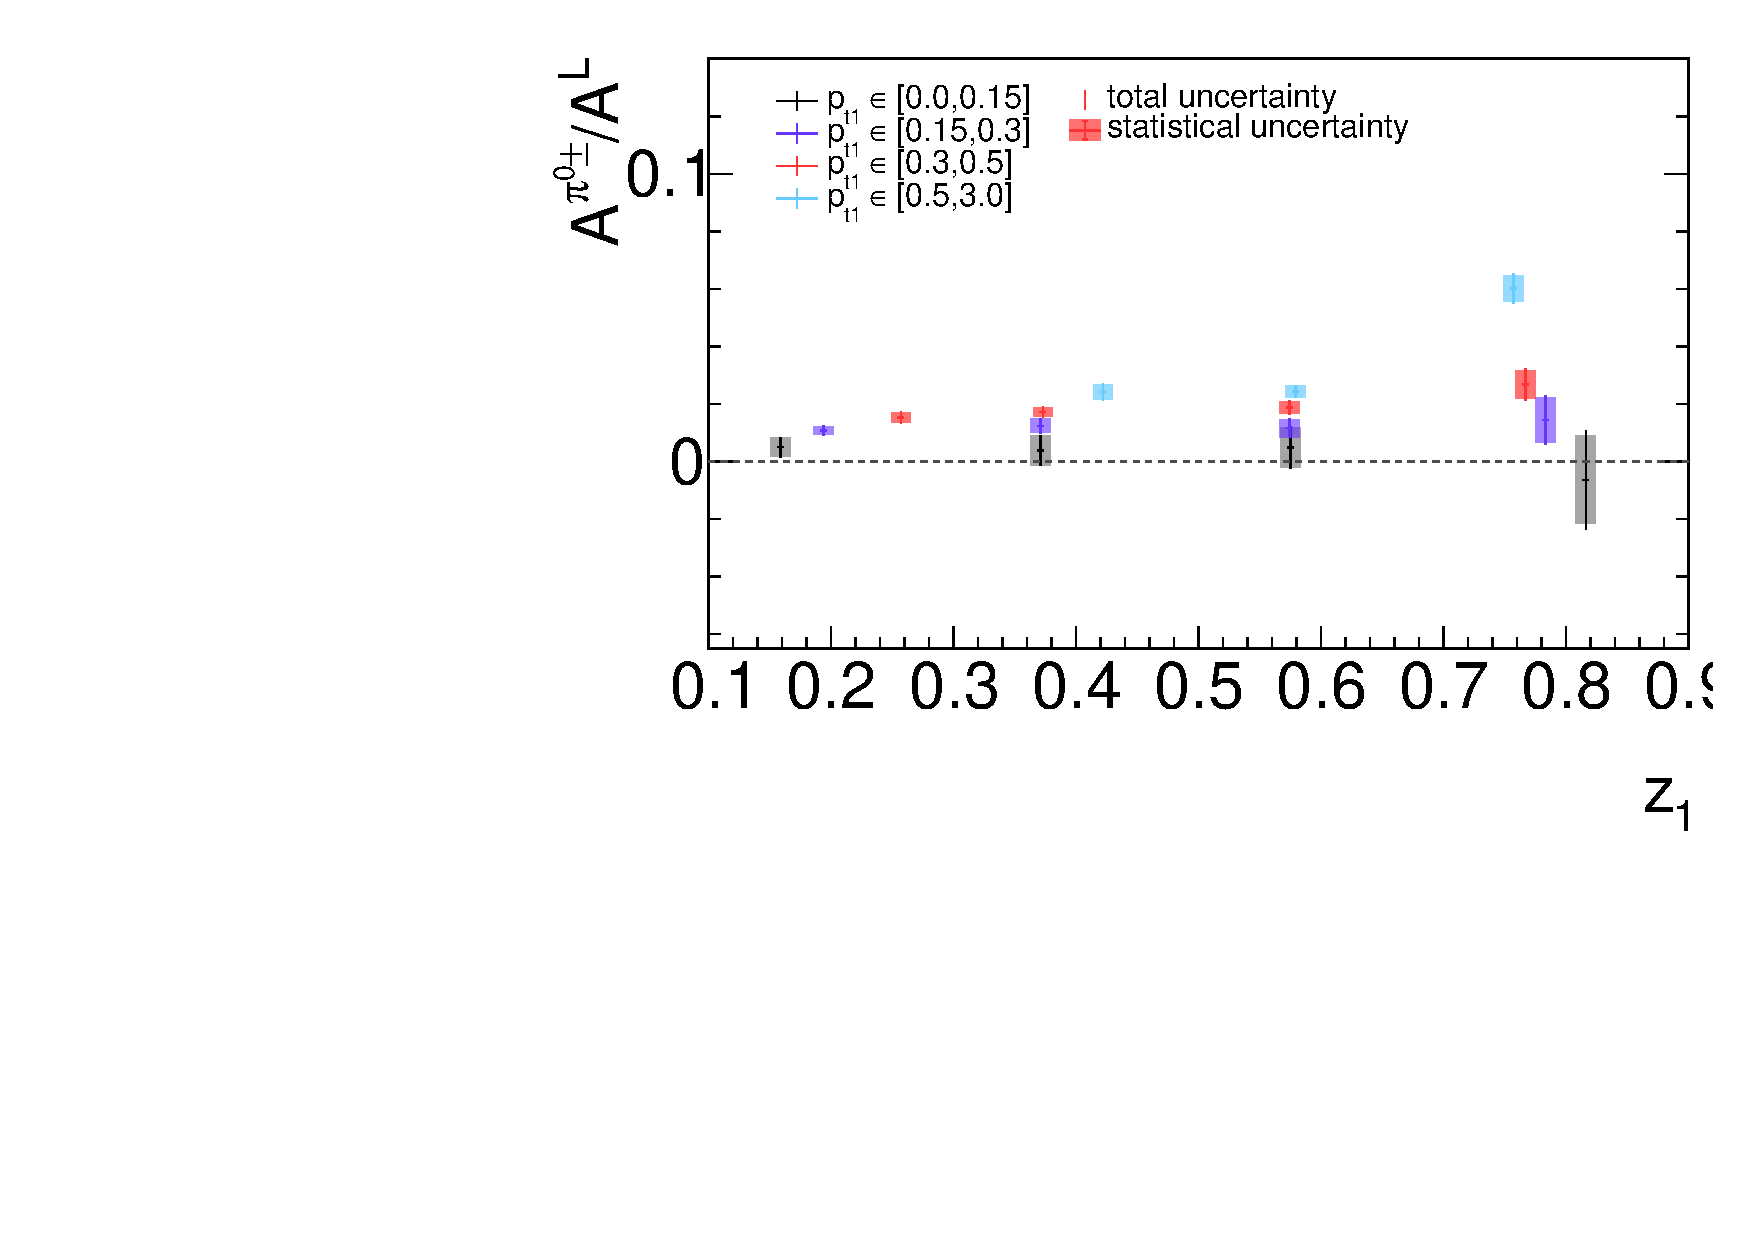
\includegraphics[width=0.45\textwidth,natwidth=200,natheight=150]{figure_asy/pi0_16bin_3.pdf}}
  \subfigure{\label{fig:16bin1}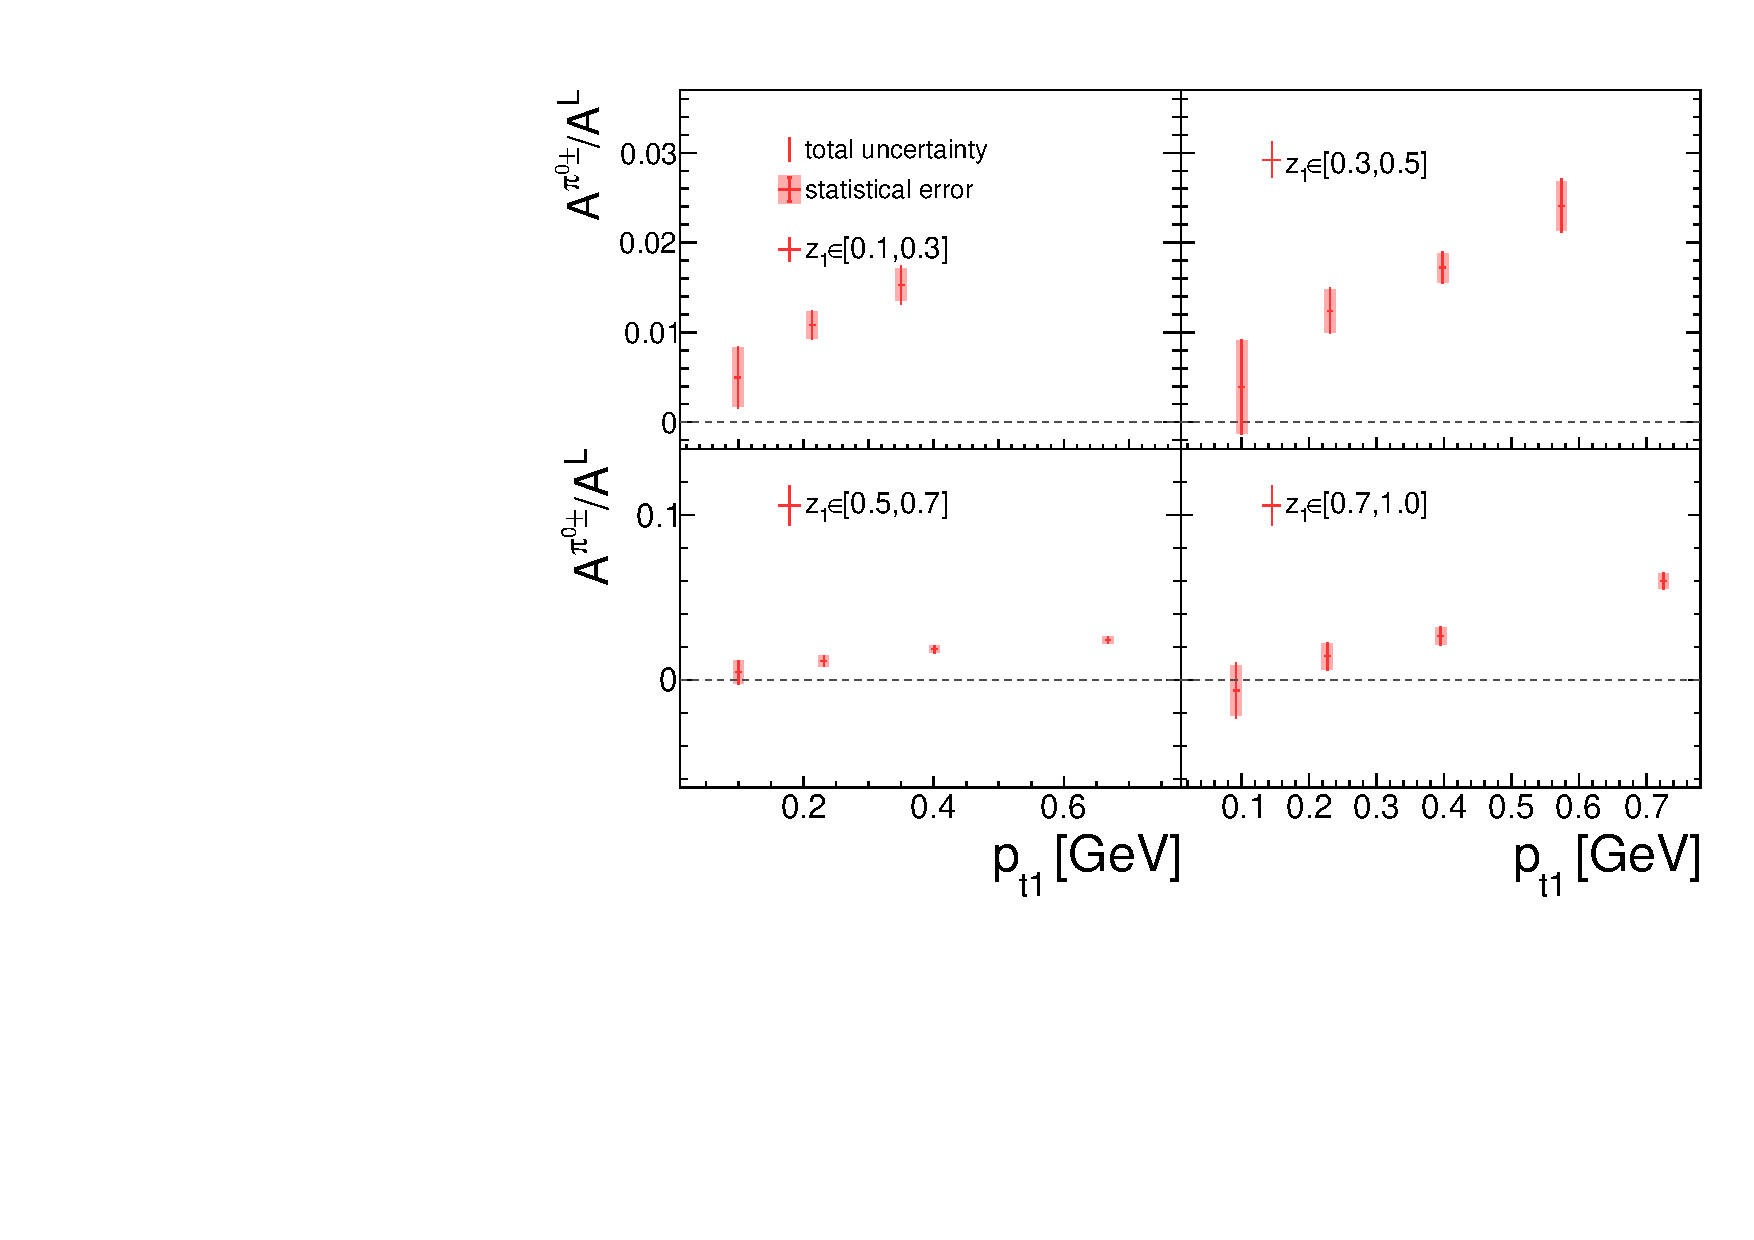
\includegraphics[width=0.45\textwidth,natwidth=200,natheight=150]{figure_asy/pi0_16bin.pdf}}
\caption{The Collins asymmetry $A_{12}$ of $\pi^0$ in the new kinematic bins discussed in section~\ref{sec:newbins}. The x coordinates of $\pi^0$ are the centroids of kinematic bins\. The inner shaded regions represent the statistical uncertainties of each data point, while the outer error bars show the total uncertainties.}
\label{fig:finalasymmetry3}
\end{figure}
\begin{figure}[H]
  \centering     
  \subfigure{\label{fig:comz2}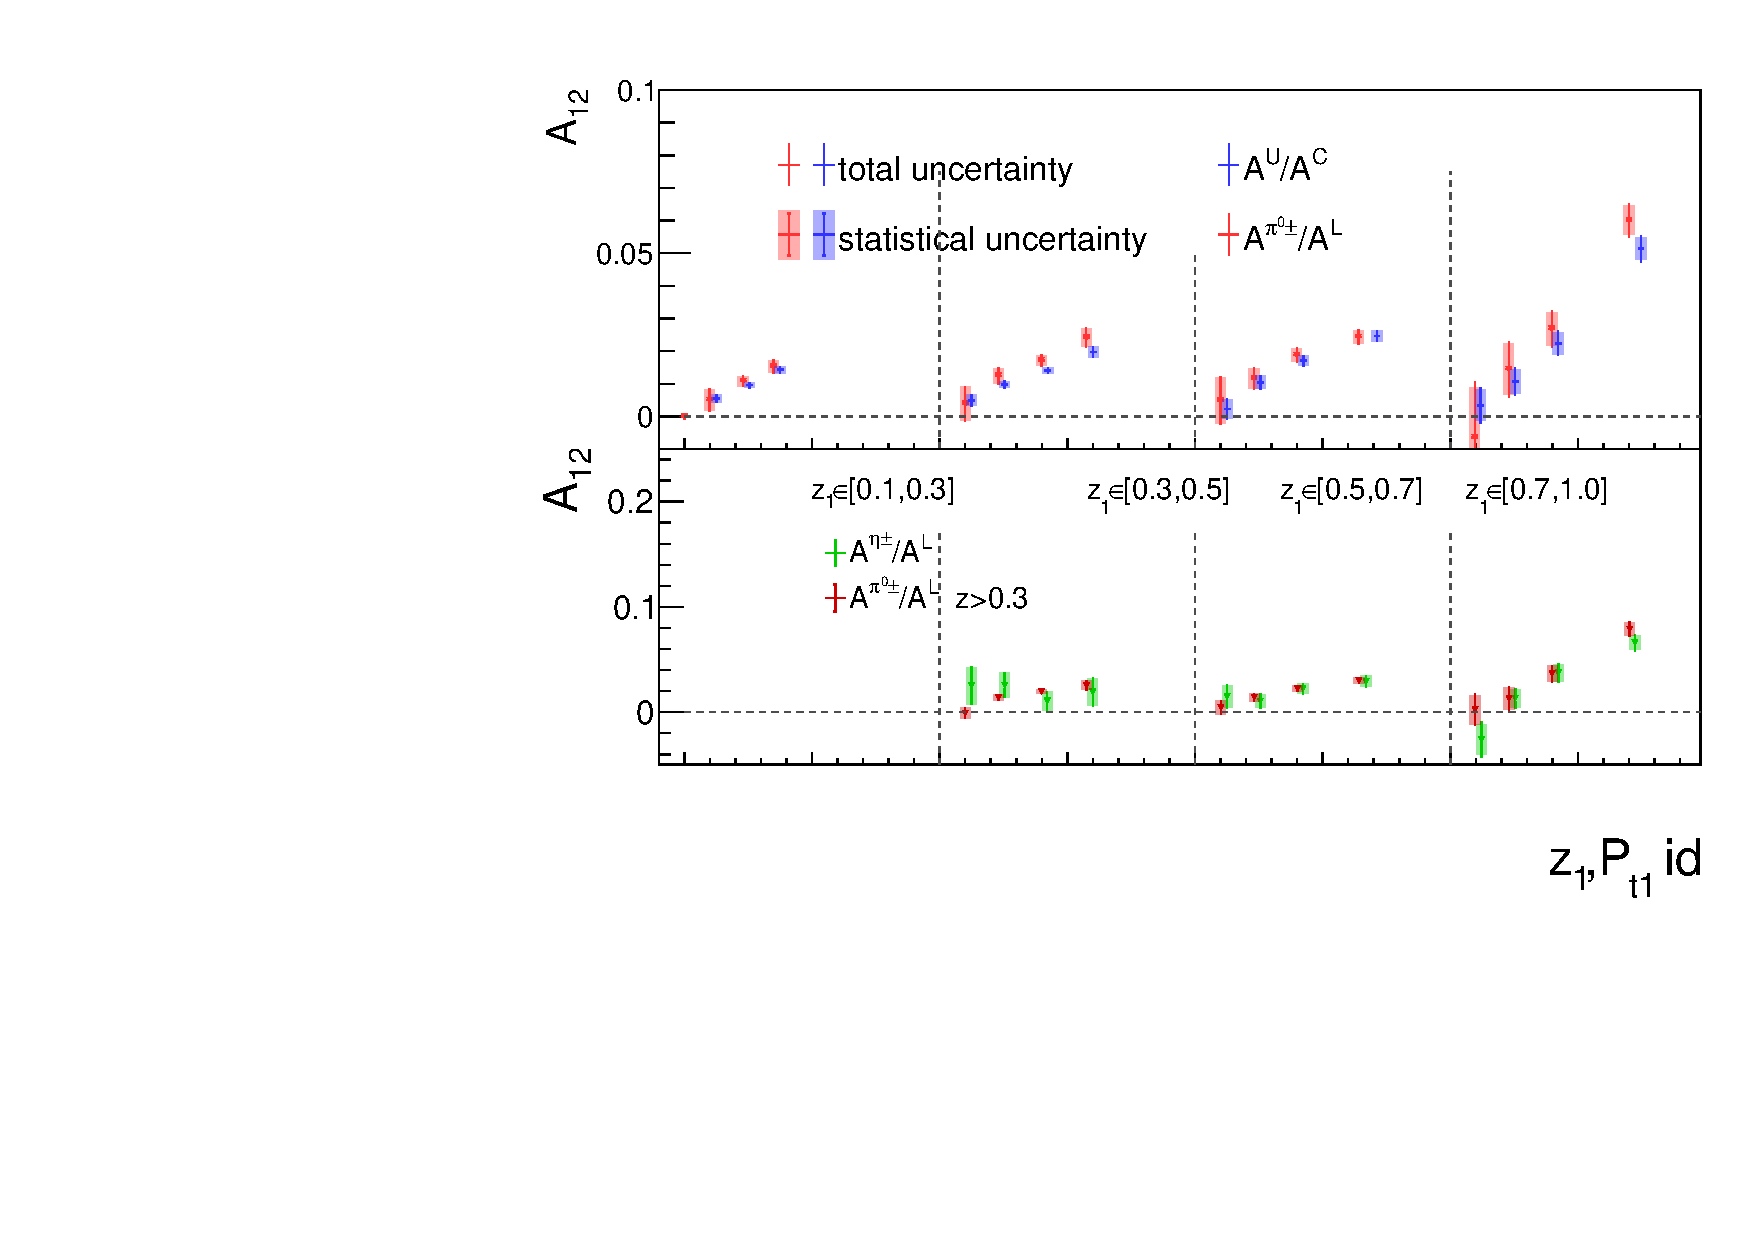
\includegraphics[width=0.45\textwidth,natwidth=200,natheight=150]{figure_asy/pi0_eta_zpt.pdf}}
\caption{ The Collins asymmetry $A_{12}$ of $\pi^0$, UC and $\eta$, separated in $z$ bins, displayed as a function of the fractional energy $P_t$. In lower panels the photon energy and $z$ criterion applied to $\eta$ are applied on $\pi^0$. The x coordinates are the centroids of kinematic bins while the horizontal position of UC and $\eta$ points are shifted to avoid overlapping. The inner shaded regions represent the statistical uncertainties of each data point, while the outer error bars show the total uncertainties.}
\label{fig:finalasymmetry5}
\end{figure}


%\textcolor{red}{Table content will be updated.}
\begin{table}[H]\scriptsize
\centering
\begin{tabular}{|c| c| c| c| c| c| c| c| c| c|c| c| c| c| c|}
\hline
$z_1$ & $\langle  z_1\rangle$ & $\langle  p_{t1}\rangle$  & $z_2$ & $\langle  z_2 \rangle$ & $\langle  p_{t2}\rangle$ & $\frac{\sin^2(\theta)}{1+\cos^2(\theta)}$& $A^{\pi^0\pm}(\%)$  \\ \hline
[0.2,0.3]	&	0.246	&	0.238	&	[0.2,1.0]	&	0.355	&	0.317	&	0.905	&	1.25  $\pm$ 0.12  $\pm$ 0.06    \\ \hline
[0.3,0.4]	&	0.345	&	0.321	&	[0.2,1.0]	&	0.356	&	0.317	&	0.906	&	1.72  $\pm$ 0.13  $\pm$ 0.04    \\ \hline
[0.4,0.5]	&	0.445	&	0.392	&	[0.2,1.0]	&	0.357	&	0.318	&	0.907	&	1.72  $\pm$ 0.16  $\pm$ 0.06    \\ \hline
[0.5,0.6]	&	0.544	&	0.449	&	[0.2,1.0]	&	0.358	&	0.318	&	0.905	&	2.08  $\pm$ 0.22  $\pm$ 0.11    \\ \hline
[0.6,0.7]	&	0.643	&	0.485	&	[0.2,1.0]	&	0.359	&	0.32	&	0.904	&	2.51  $\pm$ 0.28  $\pm$ 0.13    \\ \hline
[0.7,1.0]	&	0.77	&	0.442	&	[0.2,1.0]	&	0.359	&	0.321	&	0.902	&	3.86  $\pm$ 0.36  $\pm$ 0.2  	\\ \hline
																				
[0.1,0.2]	&	0.149	&	0.146	&	[0.1,0.2]	&	0.148	&	0.15	&	0.906	&0.16  $\pm$ 0.19  $\pm$ 0.04 	\\ \hline
[0.1,0.2]	&	0.149	&	0.147	&	[0.2,0.3]	&	0.246	&	0.241	&	0.905	&0.18  $\pm$ 0.22  $\pm$ 0.06 	\\ \hline
[0.1,0.2]	&	0.149	&	0.147	&	[0.3,0.5]	&	0.381	&	0.348	&	0.905	&0.47  $\pm$ 0.22  $\pm$ 0.07 	\\ \hline
[0.1,0.2]	&	0.149	&	0.147	&	[0.5,0.7]	&	0.577	&	0.458	&	0.905	&1.02  $\pm$ 0.41  $\pm$ 0.11 	\\ \hline
[0.1,0.2]	&	0.149	&	0.148	&	[0.7,1.0]	&	0.776	&	0.425	&	0.903	&2.52  $\pm$ 0.92  $\pm$ 0.25 	\\ \hline
[0.2,0.3]	&	0.246	&	0.238	&	[0.1,0.2]	&	0.148	&	0.15	&	0.906	&0.74  $\pm$ 0.15  $\pm$ 0.04 	\\ \hline
[0.2,0.3]	&	0.246	&	0.238	&	[0.2,0.3]	&	0.246	&	0.242	&	0.906	&1.07  $\pm$ 0.19  $\pm$ 0.05 	\\ \hline
[0.2,0.3]	&	0.246	&	0.238	&	[0.3,0.5]	&	0.381	&	0.348	&	0.905	&1.07  $\pm$ 0.19  $\pm$ 0.11 	\\ \hline
[0.2,0.3]	&	0.246	&	0.238	&	[0.5,0.7]	&	0.578	&	0.46	&	0.905	&1.85  $\pm$ 0.37  $\pm$ 0.12 	\\ \hline
[0.2,0.3]	&	0.246	&	0.24	&	[0.7,1.0]	&	0.777	&	0.434	&	0.903	&4.33  $\pm$ 0.77  $\pm$ 0.32 	\\ \hline
[0.3,0.5]	&	0.38	&	0.345	&	[0.1,0.2]	&	0.148	&	0.15	&	0.908	&0.71  $\pm$ 0.13  $\pm$ 0.04 	\\ \hline
[0.3,0.5]	&	0.38	&	0.345	&	[0.2,0.3]	&	0.246	&	0.242	&	0.907	&1.4  $\pm$ 0.15  $\pm$ 0.05  	\\ \hline
[0.3,0.5]	&	0.38	&	0.346	&	[0.3,0.5]	&	0.381	&	0.348	&	0.906	&1.63  $\pm$ 0.16  $\pm$ 0.06 	\\ \hline
[0.3,0.5]	&	0.381	&	0.346	&	[0.5,0.7]	&	0.578	&	0.462	&	0.906	&2.83  $\pm$ 0.3  $\pm$ 0.1   	\\ \hline
[0.3,0.5]	&	0.38	&	0.347	&	[0.7,1.0]	&	0.777	&	0.438	&	0.905	&4.07  $\pm$ 0.65  $\pm$ 0.28 	\\ \hline
[0.5,0.7]	&	0.575	&	0.457	&	[0.1,0.2]	&	0.149	&	0.151	&	0.906	&1.46  $\pm$ 0.22  $\pm$ 0.09 	\\ \hline
[0.5,0.7]	&	0.575	&	0.459	&	[0.2,0.3]	&	0.246	&	0.242	&	0.905	&1.54  $\pm$ 0.26  $\pm$ 0.16 	\\ \hline
[0.5,0.7]	&	0.576	&	0.461	&	[0.3,0.5]	&	0.382	&	0.348	&	0.905	&2.49  $\pm$ 0.26  $\pm$ 0.1  	\\ \hline
[0.5,0.7]	&	0.576	&	0.464	&	[0.5,0.7]	&	0.579	&	0.464	&	0.905	&3.39  $\pm$ 0.49  $\pm$ 0.24 	\\ \hline
[0.5,0.7]	&	0.576	&	0.466	&	[0.7,1.0]	&	0.777	&	0.442	&	0.904	&4.94  $\pm$ 1.06  $\pm$ 0.6  	\\ \hline
[0.7,1.0]	&	0.769	&	0.425	&	[0.1,0.2]	&	0.149	&	0.151	&	0.902	&1.56  $\pm$ 0.45  $\pm$ 0.26 	\\ \hline
[0.7,1.0]	&	0.77	&	0.438	&	[0.2,0.3]	&	0.246	&	0.242	&	0.902	&1.53  $\pm$ 0.53  $\pm$ 0.28 	\\ \hline
[0.7,1.0]	&	0.77	&	0.443	&	[0.3,0.5]	&	0.382	&	0.349	&	0.901	&4.95  $\pm$ 0.57  $\pm$ 0.31 	\\ \hline
[0.7,1.0]	&	0.77	&	0.45	&	[0.5,0.7]	&	0.578	&	0.466	&	0.903	&6.17  $\pm$ 1.04  $\pm$ 0.64 	\\ \hline
[0.7,1.0]	&	0.766	&	0.465	&	[0.7,1.0]	&	0.771	&	0.461	&	0.903	&18.92 $\pm$ 2.49  $\pm$ 2.64	\\ \hline
\end{tabular}
\caption{Azimuthal asymmetries of $\pi^0$ in $z$ bins. Uncertainties are statistical and systematic.}
\label{tab:finalpi0zbin}
\end{table}

\begin{table}[H]\scriptsize
\centering
\begin{tabular}{|c| c| c| c| c| c| c| c| c| c|c| c| c| c| c|}
\hline
$z_1$ & $\langle  z_1\rangle$ & $\langle  p_{t1} \rangle$ & $z_2$ & $\langle  z_2 \rangle$ & $\langle  p_{t2}  \rangle$& $\frac{\sin^2(\theta)}{1+\cos^2(\theta)}$ & $A^{\eta\pm}(\%)$  \\ \hline
[0.2,0.3]	&		&		&	[0.2,1.0]	&		&		&		&		$\pm$			/+		\\ \hline
[0.3,0.4]	&	0.348	&	0.303	&	[0.2,1.0]	&	0.441	&	0.375	&	0.906	&2.52  $\pm$ 0.89  $\pm$ 0.11   \\ \hline
[0.4,0.5]	&	0.446	&	0.375	&	[0.2,1.0]	&	0.442	&	0.376	&	0.907	&2.61  $\pm$ 0.65  $\pm$ 0.14   \\ \hline
[0.5,0.6]	&	0.545	&	0.433	&	[0.2,1.0]	&	0.443	&	0.376	&	0.907	&2.82  $\pm$ 0.6  $\pm$ 0.2     \\ \hline
[0.6,0.7]	&	0.644	&	0.469	&	[0.2,1.0]	&	0.442	&	0.378	&	0.908	&2.63  $\pm$ 0.65  $\pm$ 0.31   \\ \hline
[0.7,1.0]	&	0.774	&	0.43	&	[0.2,1.0]	&	0.441	&	0.379	&	0.906	&2.8  $\pm$ 0.64  $\pm$ 0.42    \\ \hline
[0.1,0.2]	&		&		&	[0.1,0.2]	&		&		&		&							\\ \hline
[0.1,0.2]	&		&		&	[0.2,0.3]	&		&		&		&							\\ \hline
[0.1,0.2]	&		&		&	[0.3,0.5]	&		&		&		&							\\ \hline
[0.1,0.2]	&		&		&	[0.5,0.7]	&		&		&		&							\\ \hline
[0.1,0.2]	&		&		&	[0.7,1.0]	&		&		&		&							\\ \hline
[0.2,0.3]	&		&		&	[0.1,0.2]	&		&		&		&							\\ \hline
[0.2,0.3]	&		&		&	[0.2,0.3]	&		&		&		&							\\ \hline
[0.2,0.3]	&		&		&	[0.3,0.5]	&		&		&		&							\\ \hline
[0.2,0.3]	&		&		&	[0.5,0.7]	&		&		&		&							\\ \hline
[0.2,0.3]	&		&		&	[0.7,1.0]	&		&		&		&							\\ \hline
[0.3,0.5]	&		&		&	[0.1,0.2]	&		&		&		&							\\ \hline
[0.3,0.5]	&		&		&	[0.2,0.3]	&		&		&		&							\\ \hline
[0.3,0.5]	&	0.386	&	0.331	&	[0.3,0.5]	&	0.381	&	0.347	&	0.906	&	2.15  $\pm$ 0.63  $\pm$ 0.1     \\ \hline
[0.3,0.5]	&	0.387	&	0.331	&	[0.5,0.7]	&	0.578	&	0.461	&	0.907	&	3.59  $\pm$ 1.13  $\pm$ 0.19    \\ \hline
[0.3,0.5]	&	0.387	&	0.332	&	[0.7,1.0]	&	0.777	&	0.434	&	0.905	&	3.25  $\pm$ 2.38  $\pm$ 0.5  	\\ \hline
[0.5,0.7]	&		&		&	[0.1,0.2]	&		&		&		&							\\ \hline
[0.5,0.7]	&		&		&	[0.2,0.3]	&		&		&		&							\\ \hline
[0.5,0.7]	&	0.579	&	0.445	&	[0.3,0.5]	&	0.382	&	0.348	&	0.907	&  2.15  $\pm$ 0.51  $\pm$ 0.19  \\ \hline
[0.5,0.7]	&	0.579	&	0.447	&	[0.5,0.7]	&	0.578	&	0.463	&	0.908	&  4.91  $\pm$ 0.98  $\pm$ 0.4   \\ \hline
[0.5,0.7]	&	0.578	&	0.447	&	[0.7,1.0]	&	0.777	&	0.44	&	0.907	&  3.84  $\pm$ 2.18  $\pm$ 1.1   \\ \hline
[0.7,1.0]	&		&		&	[0.1,0.2]	&		&		&		&							\\ \hline
[0.7,1.0]	&		&		&	[0.2,0.3]	&		&		&		&							\\ \hline
[0.7,1.0]	&	0.774	&	0.427	&	[0.3,0.5]	&	0.381	&	0.349	&	0.907	& 2.17  $\pm$ 0.73  $\pm$ 0.46  	\\ \hline
[0.7,1.0]	&	0.774	&	0.434	&	[0.5,0.7]	&	0.578	&	0.466	&	0.906	& 3.15  $\pm$ 1.38  $\pm$ 0.96     \\ \hline
[0.7,1.0]	&	0.77	&	0.451	&	[0.7,1.0]	&	0.771	&	0.462	&	0.904	& 15.42  $\pm$ 3.99  $\pm$ 4.05    \\ \hline
\end{tabular}
\caption{Azimuthal asymmetries of $\eta$ in $z$ bins. Uncertainties are statistical and systematic.}
\label{tab:finaletazbin}
\end{table}

\begin{table}[H]\scriptsize
\centering
\begin{tabular}{|c| c| c| c| c| c| c| c| c| c|c| c| c| c| c|}
\hline
$z_1$ & $\langle  z_1\rangle$ & $\langle  P_{t1} \rangle$ & $z_2$ & $\langle  z_2 \rangle$ & $\langle  P_{t2}  \rangle$& $\frac{\sin^2(\theta)}{1+\cos^2(\theta)}$ & $A^{\pi^0\pm}(\%)$  \\ \hline
[0.2,0.3]	&		&		&	[0.2,1.0]	&		&		&		&							\\ \hline
[0.3,0.4]	&	0.345	&	0.321	&	[0.2,1.0]	&	0.442	&	0.376	&	0.906	& 2.19  $\pm$ 0.09  $\pm$ 0.22    	\\ \hline
[0.4,0.5]	&	0.445	&	0.392	&	[0.2,1.0]	&	0.442	&	0.377	&	0.906	& 2  $\pm$ 0.22  $\pm$ 0.08       	\\ \hline
[0.5,0.6]	&	0.544	&	0.45	&	[0.2,1.0]	&	0.443	&	0.377	&	0.905	& 2.65  $\pm$ 0.29  $\pm$ 0.11    	\\ \hline
[0.6,0.7]	&	0.643	&	0.488	&	[0.2,1.0]	&	0.444	&	0.379	&	0.904	& 3.02  $\pm$ 0.37  $\pm$ 0.17    	\\ \hline
[0.7,1.0]	&	0.769	&	0.445	&	[0.2,1.0]	&	0.443	&	0.381	&	0.902	& 5.76  $\pm$ 0.49  $\pm$ 0.28    	\\ \hline
[0.1,0.2]	&		&		&	[0.1,0.2]	&		&		&		&							\\ \hline
[0.1,0.2]	&		&		&	[0.2,0.3]	&		&		&		&							\\ \hline
[0.1,0.2]	&		&		&	[0.3,0.5]	&		&		&		&							\\ \hline
[0.1,0.2]	&		&		&	[0.5,0.7]	&		&		&		&							\\ \hline
[0.1,0.2]	&		&		&	[0.7,1.0]	&		&		&		&							\\ \hline
[0.2,0.3]	&		&		&	[0.1,0.2]	&		&		&		&							\\ \hline
[0.2,0.3]	&		&		&	[0.2,0.3]	&		&		&		&							\\ \hline
[0.2,0.3]	&		&		&	[0.3,0.5]	&		&		&		&							\\ \hline
[0.2,0.3]	&		&		&	[0.5,0.7]	&		&		&		&							\\ \hline
[0.2,0.3]	&		&		&	[0.7,1.0]	&		&		&		&							\\ \hline
[0.3,0.5]	&		&		&	[0.1,0.2]	&		&		&		&							\\ \hline
[0.3,0.5]	&		&		&	[0.2,0.3]	&		&		&		&							\\ \hline
[0.3,0.5]	&	0.38	&	0.346	&	[0.3,0.5]	&	0.381	&	0.348	&	0.906	& 1.63  $\pm$ 0.16  $\pm$ 0.06  	\\ \hline
[0.3,0.5]	&	0.381	&	0.346	&	[0.5,0.7]	&	0.578	&	0.462	&	0.906	& 2.83  $\pm$ 0.3  $\pm$ 0.1    	\\ \hline
[0.3,0.5]	&	0.38	&	0.347	&	[0.7,1.0]	&	0.777	&	0.438	&	0.905	& 4.07  $\pm$ 0.65  $\pm$ 0.28  	\\ \hline
[0.5,0.7]	&		&		&	[0.1,0.2]	&		&		&		&							\\ \hline
[0.5,0.7]	&		&		&	[0.2,0.3]	&		&		&		&							\\ \hline
[0.5,0.7]	&	0.576	&	0.461	&	[0.3,0.5]	&	0.382	&	0.348	&	0.905	&2.49  $\pm$ 0.26  $\pm$ 0.1  	\\ \hline
[0.5,0.7]	&	0.576	&	0.464	&	[0.5,0.7]	&	0.579	&	0.464	&	0.905	&3.39  $\pm$ 0.49  $\pm$ 0.24 	\\ \hline
[0.5,0.7]	&	0.576	&	0.466	&	[0.7,1.0]	&	0.777	&	0.442	&	0.904	&4.94  $\pm$ 1.06  $\pm$ 0.6  	\\ \hline
[0.7,1.0]	&		&		&	[0.1,0.2]	&		&		&		&							\\ \hline
[0.7,1.0]	&		&		&	[0.2,0.3]	&		&		&		&							\\ \hline
[0.7,1.0]	&	0.77	&	0.443	&	[0.3,0.5]	&	0.382	&	0.349	&	0.901	&4.95  $\pm$ 0.57  $\pm$ 0.31 	\\ \hline
[0.7,1.0]	&	0.77	&	0.45	&	[0.5,0.7]	&	0.578	&	0.466	&	0.903	&6.17  $\pm$ 1.04  $\pm$ 0.64 	\\ \hline
[0.7,1.0]	&	0.766	&	0.465	&	[0.7,1.0]	&	0.771	&	0.461	&	0.903	&18.92  $\pm$ 2.49  $\pm$ 2.64	\\ \hline
\end{tabular}
\caption{Azimuthal asymmetries of $\pi^0$ with $z>0.3$ in $z$ bins. Uncertainties are statistical and systematic.}
\label{tab:finaletazbin2}
\end{table}

%\begin{landscape}
\begin{table}[H]\scriptsize
\centering
\renewcommand{\arraystretch}{1.5}
%\resizebox{1.2\textwidth}{!}{
\begin{tabular}{|c|c|c|c|c|c|c|c|c|}
\hline
$z_1$ & $\langle  z_1 \rangle$ & $\langle  P_{t1}  \rangle$ & $z_2$ &  $\langle  z_2 \rangle$ & $\langle  P_{t2}\rangle$  &$\frac{\sin^2(\theta)}{1+\cos^2(\theta)}$ & $A^{UL}(\%)$ &  $A^{UC}(\%)$   \\ \hline
[0.2,0.3]	&	0.247	&	0.241	&	[0.2,1.0]	&	0.358	&	0.317	&	0.904	&2.47  $\pm$ 0.09  $\pm$ 0.03 &1.24  $\pm$ 0.08  $\pm$ 0.03 \\ \hline
[0.3,0.4]	&	0.346	&	0.322	&	[0.2,1.0]	&	0.354	&	0.315	&	0.906	&2.75  $\pm$ 0.12  $\pm$ 0.04 &1.38  $\pm$ 0.09  $\pm$ 0.03 \\ \hline
[0.4,0.5]	&	0.445	&	0.392	&	[0.2,1.0]	&	0.353	&	0.315	&	0.907	&2.85  $\pm$ 0.16  $\pm$ 0.06 &1.43  $\pm$ 0.12  $\pm$ 0.04 \\ \hline
[0.5,0.6]	&	0.545	&	0.449	&	[0.2,1.0]	&	0.355	&	0.316	&	0.906	&3.86  $\pm$ 0.22  $\pm$ 0.08 &1.93  $\pm$ 0.17  $\pm$ 0.06 \\ \hline
[0.6,0.7]	&	0.644	&	0.484	&	[0.2,1.0]	&	0.356	&	0.317	&	0.906	&4.64  $\pm$ 0.29  $\pm$ 0.13 &2.32  $\pm$ 0.22  $\pm$ 0.1  \\ \hline
[0.7,1.0]	&	0.777	&	0.439	&	[0.2,1.0]	&	0.359	&	0.321	&	0.904	&6.81  $\pm$ 0.36  $\pm$ 0.2  &3.41  $\pm$ 0.27  $\pm$ 0.15 \\ \hline
[0.1,0.2]	&	0.148	&	0.150	&	[0.1,0.2]	&	0.148	&	0.150	&	0.906	&0.87  $\pm$ 0.11  $\pm$ 0.04   &	0.44  $\pm$ 0.09  $\pm$ 0.04  \\ \hline
[0.1,0.2]	&	0.148	&	0.150	&	[0.2,0.3]	&	0.246	&	0.241	&	0.905	&1.16  $\pm$ 0.13  $\pm$ 0.05   &	0.58  $\pm$ 0.1  $\pm$ 0.04   \\ \hline
[0.1,0.2]	&	0.148	&	0.150	&	[0.3,0.5]	&	0.382	&	0.347	&	0.904	&1.44  $\pm$ 0.12  $\pm$ 0.05   &	0.72  $\pm$ 0.1  $\pm$ 0.04   \\ \hline
[0.1,0.2]	&	0.148	&	0.151	&	[0.5,0.7]	&	0.578	&	0.457	&	0.904	&2.49  $\pm$ 0.23  $\pm$ 0.1    &	1.25  $\pm$ 0.18  $\pm$ 0.08  \\ \hline
[0.1,0.2]	&	0.149	&	0.151	&	[0.7,1.0]	&	0.778	&	0.421	&	0.903	&3.76  $\pm$ 0.52  $\pm$ 0.3    &	1.88  $\pm$ 0.41  $\pm$ 0.24  \\ \hline
[0.2,0.3]	&	0.247	&	0.241	&	[0.1,0.2]	&	0.148	&	0.150	&	0.906	&1.2  $\pm$ 0.12  $\pm$ 0.04    &	0.6  $\pm$ 0.1  $\pm$ 0.04    \\ \hline
[0.2,0.3]	&	0.247	&	0.241	&	[0.2,0.3]	&	0.246	&	0.241	&	0.905	&1.98  $\pm$ 0.15  $\pm$ 0.05   &	0.99  $\pm$ 0.12  $\pm$ 0.04  \\ \hline
[0.2,0.3]	&	0.247	&	0.241	&	[0.3,0.5]	&	0.382	&	0.347	&	0.904	&2.35  $\pm$ 0.14  $\pm$ 0.05   &	1.18  $\pm$ 0.11  $\pm$ 0.04  \\ \hline
[0.2,0.3]	&	0.247	&	0.241	&	[0.5,0.7]	&	0.578	&	0.459	&	0.904	&3.97  $\pm$ 0.27  $\pm$ 0.11   &	1.99  $\pm$ 0.21  $\pm$ 0.08  \\ \hline
[0.2,0.3]	&	0.247	&	0.243	&	[0.7,1.0]	&	0.778	&	0.433	&	0.903	&4.62  $\pm$ 0.55  $\pm$ 0.28   &	2.31  $\pm$ 0.42  $\pm$ 0.22  \\ \hline
[0.3,0.5]	&	0.382	&	0.345	&	[0.1,0.2]	&	0.148	&	0.150	&	0.908	&1.17  $\pm$ 0.12  $\pm$ 0.04   &	0.58  $\pm$ 0.09  $\pm$ 0.04  \\ \hline
[0.3,0.5]	&	0.382	&	0.345	&	[0.2,0.3]	&	0.246	&	0.242	&	0.907	&2.03  $\pm$ 0.14  $\pm$ 0.05   &	1.01  $\pm$ 0.11  $\pm$ 0.04  \\ \hline
[0.3,0.5]	&	0.382	&	0.349	&	[0.3,0.5]	&	0.382	&	0.348	&	0.906	&2.97  $\pm$ 0.15  $\pm$ 0.05   &	1.48  $\pm$ 0.12  $\pm$ 0.04  \\ \hline
[0.3,0.5]	&	0.382	&	0.349	&	[0.5,0.7]	&	0.578	&	0.462	&	0.906	&4.41  $\pm$ 0.28  $\pm$ 0.11   &	2.21  $\pm$ 0.22  $\pm$ 0.08  \\ \hline
[0.3,0.5]	&	0.382	&	0.350	&	[0.7,1.0]	&	0.779	&	0.436	&	0.905	&5.95  $\pm$ 0.56  $\pm$ 0.29   &	2.97  $\pm$ 0.43  $\pm$ 0.22  \\ \hline
[0.5,0.7]	&	0.578	&	0.455	&	[0.1,0.2]	&	0.148	&	0.150	&	0.908	&2.01  $\pm$ 0.22  $\pm$ 0.09   &	1.01  $\pm$ 0.17  $\pm$ 0.07  \\ \hline
[0.5,0.7]	&	0.578	&	0.458	&	[0.2,0.3]	&	0.246	&	0.242	&	0.906	&3.09  $\pm$ 0.26  $\pm$ 0.1    &	1.54  $\pm$ 0.2  $\pm$ 0.08   \\ \hline
[0.5,0.7]	&	0.579	&	0.463	&	[0.3,0.5]	&	0.382	&	0.348	&	0.905	&4.33  $\pm$ 0.28  $\pm$ 0.1    &	2.17  $\pm$ 0.22  $\pm$ 0.08  \\ \hline
[0.5,0.7]	&	0.579	&	0.466	&	[0.5,0.7]	&	0.579	&	0.465	&	0.905	&6.09  $\pm$ 0.5  $\pm$ 0.22    &	3.06  $\pm$ 0.38  $\pm$ 0.17  \\ \hline
[0.5,0.7]	&	0.580	&	0.471	&	[0.7,1.0]	&	0.780	&	0.440	&	0.906	&11.1  $\pm$ 1.05  $\pm$ 0.65   &	5.59  $\pm$ 0.77  $\pm$ 0.49  \\ \hline
[0.7,1.0]	&	0.775	&	0.424	&	[0.1,0.2]	&	0.149	&	0.151	&	0.906	&2.57  $\pm$ 0.48  $\pm$ 0.26   &	1.28  $\pm$ 0.36  $\pm$ 0.21  \\ \hline
[0.7,1.0]	&	0.777	&	0.434	&	[0.2,0.3]	&	0.247	&	0.242	&	0.905	&5.07  $\pm$ 0.53  $\pm$ 0.29   &	2.55  $\pm$ 0.4  $\pm$ 0.22   \\ \hline
[0.7,1.0]	&	0.778	&	0.441	&	[0.3,0.5]	&	0.382	&	0.350	&	0.904	&6.72  $\pm$ 0.57  $\pm$ 0.29   &	3.37  $\pm$ 0.44  $\pm$ 0.23  \\ \hline
[0.7,1.0]	&	0.779	&	0.444	&	[0.5,0.7]	&	0.579	&	0.470	&	0.904	&8.76  $\pm$ 0.96  $\pm$ 0.58   &	4.39  $\pm$ 0.71  $\pm$ 0.43  \\ \hline
[0.7,1.0]	&	0.777	&	0.461	&	[0.7,1.0]	&	0.778	&	0.464	&	0.902	&25.38  $\pm$ 2.43  $\pm$ 2.4   &	12.81  $\pm$ 1.7  $\pm$ 1.78  \\ \hline
\end{tabular}
\caption{Azimuthal asymmetries of UL and UC in $z$ bins. Uncertainties are statistical and systematic.}
\label{tab:finaluluczbin}
\end{table} 
%\end{landscape}

\begin{table}[H]\scriptsize
\centering
\begin{tabular}{|c| c| c| c| c| c| c| c| c| c|}
\hline
$P_{t1}$   & $\langle  P_{t1}  \rangle$ & $\langle  z_1 \rangle$& $P_{t2}$  & $\langle  P_{t2}\rangle$  &  $\langle  z_2 \rangle$  &$\frac{\sin^2(\theta)}{1+\cos^2(\theta)}$&  $A^{\pi^0\pm}(\%)$  \\ \hline
[0,0.15]	&	0.099	&	0.306	&	[0,3.0]	&	0.318	&	0.355	&	0.906	&     0.52  $\pm$ 0.26  $\pm$ 0.1 	\\ \hline
[0.15,0.3]	&	0.23	        &	0.305	&	[0,3.0]	&	0.317	&	0.355	&	0.905  &1.16  $\pm$ 0.12  $\pm$ 0.05 	\\ \hline
[0.3,0.5]	&	0.38	        &	0.355	&	[0,3.0]	&	0.317	&	0.356	&	0.906 & 1.71  $\pm$ 0.1  $\pm$ 0.08   	\\ \hline
[0.5,3.0]	&	0.619	&	0.502	&	[0,3.0]	&	0.317	&	0.358	&	0.906	&     2.95  $\pm$ 0.16  $\pm$ 0.08 	\\ \hline
														
[0,0.15]	&	0.099	&	0.305	&	[0,0.15]	&	0.1	        &	0.315	&	0.905	&0.12  $\pm$ 0.61  $\pm$ 0.14  	\\ \hline
[0,0.15]	&	0.099	&	0.305	&	[0.15,0.3]	&	0.231	&	0.311	&	0.905   	&0.49  $\pm$ 0.42  $\pm$ 0.11  	\\ \hline
[0,0.15]	&	0.1	        &	0.306	&	[0.3,0.5]	&	0.381	&	0.36	         &0.906       &0.24  $\pm$ 0.41  $\pm$ 0.17       	\\ \hline
[0,0.15]	&	0.099	&	0.308	&	[0.5,3.0]	&	0.623	&	0.51	        &	0.906	&1.83  $\pm$ 0.71  $\pm$ 0.19  		\\ \hline
[0.15,0.3]	&	0.23	        &	0.304	&	[0,0.15]	&	0.1	        &	0.316	&0.906        &0.99  $\pm$ 0.39  $\pm$ 0.11  	\\ \hline
[0.15,0.3]	&	0.23	        &	0.305	&	[0.15,0.3]	&	0.231	&	0.312	&	0.905	&0.92  $\pm$ 0.19  $\pm$ 0.05  		\\ \hline
[0.15,0.3]	&	0.23	        &	0.305	&	[0.3,0.5]	&	0.381	&	0.36	        &0.905	&1.16  $\pm$ 0.18  $\pm$ 0.08  	\\ \hline
[0.15,0.3]	&	0.23	        &	0.306	&	[0.5,3.0]	&	0.624	&	0.51	        & 0.906	& 1.92  $\pm$ 0.31  $\pm$ 0.13 	\\ \hline
[0.3,0.5]	&	0.38	        &	0.354	&	[0,0.15]	&	0.099	&	0.318	&	0.906	&0.7  $\pm$ 0.35  $\pm$ 0.12   		\\ \hline
[0.3,0.5]	&	0.38	        &	0.355	&	[0.15,0.3]	&	0.231	&	0.312	&	0.906	&1.41  $\pm$ 0.17  $\pm$ 0.08  	\\ \hline
[0.3,0.5]	&	0.38	        &	0.355	&	[0.3,0.5]	&	0.381	&	0.361	&	0.906	&1.93  $\pm$ 0.16  $\pm$ 0.08  		\\ \hline
[0.3,0.5]	&	0.38	        &	0.357	&	[0.5,3.0]	&	0.623	&	0.51	 &       0.906   &     2.74  $\pm$ 0.28  $\pm$ 0.17  			\\ \hline
[0.5,3.0]	&	0.619	&	0.502	&	[0,0.15]	&	0.1	        &	0.32	  &    0.906          &1.18  $\pm$ 0.49  $\pm$ 0.22  	\\ \hline
[0.5,3.0]	&	0.619	&	0.502	&	[0.15,0.3]	&	0.231	&	0.314	&	0.905    	&2.43  $\pm$ 0.25  $\pm$ 0.11  	\\ \hline
[0.5,3.0]	&	0.619	&	0.503	&	[0.3,0.5]	&	0.381	&	0.363	&	0.906    	&2.72  $\pm$ 0.24  $\pm$ 0.1   	\\ \hline
[0.5,3.0]	&	0.618	&	0.503	&	[0.5,3.0]	&	0.623	&	0.511	&	0.906   	&5.87  $\pm$ 0.48  $\pm$ 0.24  	\\ \hline
\end{tabular}
\caption{Azimuthal asymmetries of $\pi^0$ in $P_t$ bins. Uncertainties are statistical and systematic.}
\label{tab:finalpi0ptbin}
\end{table}

\begin{table}[H]\scriptsize
\centering
\begin{tabular}{|c| c| c| c| c| c| c| c| c| c|}
\hline
$P_{t1}$   & $\langle  p_{t1} \rangle$(GeV) & $\langle  z_1 \rangle$& $P_{t2}$  & $\langle  p_{t2}\rangle$  &  $\langle  z_2 \rangle$  &$\frac{\sin^2(\theta)}{1+\cos^2(\theta)}$&  $A^{\eta\pm}(\%)$  \\ \hline
[0,0.15]	&	0.099	&	0.434	&	[0,3.0]	&	0.378	&	0.44	        &	0.099	&	1.29  $\pm$ 1.2  $\pm$ 0.21  	\\ \hline
[0.15,0.3]	&	0.23	        &	0.429	&	[0,3.0]	&	0.377	&	0.441	&	0.23	    &	1.75  $\pm$ 0.64  $\pm$ 0.11 	\\ \hline
[0.3,0.5]	&	0.395	&	0.436	&	[0,3.0]	&	0.375	&	0.442	&	0.395    	&	1.81  $\pm$ 0.45  $\pm$ 0.1  	\\ \hline
[0.5,3.0]	&	0.625	&	0.526	&	[0,3.0]	&	0.373	&	0.443	&	0.625   	&	2.91  $\pm$ 0.48  $\pm$ 0.19 	\\ \hline
														
[0,0.15]	&	0.098	&	0.431	&	[0,0.15]	&	0.098	&	0.424	&	0.098	&-0.63  $\pm$ 3.45  $\pm$ 0.66 	\\ \hline
[0,0.15]	&	0.099	&	0.431	&	[0.15,0.3]	&	0.231	&	0.42	        &0.099	&-3.59  $\pm$ 3.63  $\pm$ 0.85 	\\ \hline
[0,0.15]	&	0.099	&	0.435	&	[0.3,0.5]	&	0.399	&	0.418	&	0.099	&2.66  $\pm$ 1.76  $\pm$ 0.37  	\\ \hline
[0,0.15]	&	0.099	&	0.437	&	[0.5,3.0]	&	0.624	&	0.511	&	0.099	&2.66  $\pm$ 2.07  $\pm$ 0.46  	\\ \hline
[0.15,0.3]	&	0.23	        &	0.427	&	[0,0.15]	&0.1&0.429	&	0.23	        &-1.73  $\pm$ 2.16  $\pm$ 0.48 	\\ \hline
[0.15,0.3]	&	0.23	        &	0.428	&	[0.15,0.3]	&    0.231&0.42&	0.23	        &0.34  $\pm$ 1.34  $\pm$ 0.21  	\\ \hline
[0.15,0.3]	&	0.23	        	&	0.429	&	[0.3,0.5]	&0.399	&0.419	&0.23	        &1.52  $\pm$ 0.97  $\pm$ 0.16  	\\ \hline
[0.15,0.3]	&	0.23		&	0.431	&	[0.5,3.0]	&	0.624	&0.51 &	0.23	        &4.77  $\pm$ 1.28  $\pm$ 0.27  	\\ \hline
[0.3,0.5]	&	0.396	&	0.433	&	[0,0.15]	&	0.099	&	0.431	&	0.396	&0.44  $\pm$ 1.91  $\pm$ 0.38  	\\ \hline
[0.3,0.5]	&	0.395	&	0.435	&	[0.15,0.3]	&	0.231	&	0.421	&	0.395	&0.98  $\pm$ 0.94  $\pm$ 0.19  	\\ \hline
[0.3,0.5]	&	0.395	&	0.436	&	[0.3,0.5]	&	0.398	&	0.42	        &0.395	&1.89  $\pm$ 0.69  $\pm$ 0.15  	\\ \hline
[0.3,0.5]	&	0.395	&	0.437	&	[0.5,3.0]	&	0.624	&	0.511	&	0.395	&2.95  $\pm$ 0.94  $\pm$ 0.23  	\\ \hline
[0.5,3.0]	&	0.625	&	0.527	&	[0,0.15]	&	0.1	        &	0.435	&0.625	&1.47  $\pm$ 1.66  $\pm$ 0.62  	\\ \hline
[0.5,3.0]	&	0.626	&	0.527	&	[0.15,0.3]	&	0.231	&	0.423	&	0.626	&1.22  $\pm$ 0.94  $\pm$ 0.34  	\\ \hline
[0.5,3.0]	&	0.625	&	0.526	&	[0.3,0.5]	&	0.398	&	0.422	&	0.625	&2.67  $\pm$ 0.67  $\pm$ 0.26  	\\ \hline
[0.5,3.0]	&	0.623	&	0.526	&	[0.5,3.0]	&	0.623	&	0.511	&	0.623	&5.26  $\pm$ 1.04  $\pm$ 0.46  	\\ \hline
\end{tabular}
\caption{Azimuthal asymmetries of $\eta$ in $P_t$ bins. Uncertainties are statistical and systematic.}
\label{tab:finaletaptbin}
\end{table}

\begin{table}[H]\scriptsize
\centering
\begin{tabular}{|c| c| c| c| c| c| c| c| c| c|}
\hline
$P_{t1}$   & $\langle  p_{t1} \rangle$(GeV) & $\langle  z_1 \rangle$& $P_{t2}$  & $\langle  p_{t2}\rangle$  &  $\langle  z_2 \rangle$  &$\frac{\sin^2(\theta)}{1+\cos^2(\theta)}$&  $A^{\pi^0\pm}(\%)$  \\ \hline
[0,0.15]	&	0.099	&	0.417	&	[0,3.0]	&	0.379	&	0.441	&	0.906	&	0.38  $\pm$ 0.54  $\pm$ 0.2  	\\ \hline
[0.15,0.3]	&	0.231	&	0.412	&	[0,3.0]	&	0.378	&	0.441	&	0.906	&	1.59  $\pm$ 0.24  $\pm$ 0.09    \\ \hline
[0.3,0.5]	&	0.398	&	0.414	&	[0,3.0]	&	0.377	&	0.442	&	0.906	&	2.15  $\pm$ 0.17  $\pm$ 0.1     \\ \hline
[0.5,3.0]	&	0.620	&	0.503	&	[0,3.0]	&	0.374	&	0.443	&	0.905	&	3.6  $\pm$ 0.22  $\pm$ 0.09     \\ \hline
																				
[0,0.15]	&	0.099	&	0.414	&	[0,0.15]	&	0.099	&	0.425	&	0.905	&-1.57  $\pm$ 1.88  $\pm$ 0.64   	\\ \hline
[0,0.15]	&	0.099	&	0.415	&	[0.15,0.3]	&	0.231	&	0.420	&	0.906	&0.35  $\pm$ 1.07  $\pm$ 0.37    	\\ \hline
[0,0.15]	&	0.100	&	0.417	&	[0.3,0.5]	&	0.399	&	0.419	&	0.906	&0.28  $\pm$ 0.8  $\pm$ 0.29     	\\ \hline
[0,0.15]	&	0.099	&	0.421	&	[0.5,3.0]	&	0.624	&	0.511	&	0.906	&1.1  $\pm$ 1.09  $\pm$ 0.35         	\\ \hline
[0.15,0.3]	&	0.231	&	0.410	&	[0,0.15]	&	0.100	&	0.427	&	0.906	&1.22  $\pm$ 1.13  $\pm$ 0.33    	\\ \hline
[0.15,0.3]	&	0.231	&	0.411	&	[0.15,0.3]	&	0.231	&	0.420	&	0.905	&0.61  $\pm$ 0.46  $\pm$ 0.18        	\\ \hline
[0.15,0.3]	&	0.231	&	0.412	&	[0.3,0.5]	&	0.398	&	0.419	&	0.905	&1.77  $\pm$ 0.36  $\pm$ 0.1     	\\ \hline
[0.15,0.3]	&	0.231	&	0.414	&	[0.5,3.0]	&	0.625	&	0.511	&	0.907	&2.42  $\pm$ 0.47  $\pm$ 0.16    	\\ \hline
[0.3,0.5]	&	0.399	&	0.413	&	[0,0.15]	&	0.099	&	0.431	&	0.905	&1.55  $\pm$ 0.77  $\pm$ 0.28    	\\ \hline
[0.3,0.5]	&	0.398	&	0.413	&	[0.15,0.3]	&	0.231	&	0.421	&	0.906	&1.68  $\pm$ 0.34  $\pm$ 0.12    	\\ \hline
[0.3,0.5]	&	0.398	&	0.414	&	[0.3,0.5]	&	0.398	&	0.420	&	0.906	&2.01  $\pm$ 0.24  $\pm$ 0.11    	\\ \hline
[0.3,0.5]	&	0.398	&	0.415	&	[0.5,3.0]	&	0.624	&	0.511	&	0.906	&3.13  $\pm$ 0.33  $\pm$ 0.15    	\\ \hline
[0.5,3.0]	&	0.621	&	0.503	&	[0,0.15]	&	0.099	&	0.433	&	0.905	&2.43  $\pm$ 0.86  $\pm$ 0.33    	\\ \hline
[0.5,3.0]	&	0.621	&	0.504	&	[0.15,0.3]	&	0.231	&	0.423	&	0.905	&2.7  $\pm$ 0.43  $\pm$ 0.17     	\\ \hline
[0.5,3.0]	&	0.620	&	0.503	&	[0.3,0.5]	&	0.398	&	0.422	&	0.906	&3.03  $\pm$ 0.3  $\pm$ 0.12     	\\ \hline
[0.5,3.0]	&	0.618	&	0.503	&	[0.5,3.0]	&	0.623	&	0.511	&	0.906	&5.78  $\pm$ 0.47  $\pm$ 0.24    	\\ \hline
\end{tabular}
\caption{Azimuthal asymmetries of $\pi^0$ with $z>0.3$ in $P_t$ bins. Uncertainties are statistical and systematic.}
\label{tab:finaletaptbin2}
\end{table}

\begin{table}[H]\scriptsize
\centering
\renewcommand{\arraystretch}{1.5}
\begin{tabular}{|c| c| c| c| c| c| c| c| c| c|}
\hline
$P_{t1}$ & $\langle  p_{t1} \rangle$ & $\langle  z_{1}  \rangle$ & $P_{t2}$ &  $\langle  p_{t2}\rangle$ & $\langle  z_{2}\rangle$ &$\frac{\sin^2(\theta)}{1+\cos^2(\theta)}$ &$A^{UL}(\%)$ &  $A^{UC}(\%)$   \\ \hline
[0,0.15]	&	0.100	&	0.319	&	[0,3.0]	&	0.317	&	0.355	&	0.905	& 1.34  $\pm$ 0.19  $\pm$ 0.07 & 0.67  $\pm$ 0.15  $\pm$ 0.05 \\ \hline
[0.15,0.3]	&	0.231	&	0.314	&	[0,3.0]	&	0.317	&	0.355	&	0.905	& 2.25  $\pm$ 0.1  $\pm$ 0.03  & 1.12  $\pm$ 0.08  $\pm$ 0.03 \\ \hline
[0.3,0.5]	&	0.381	&	0.364	&	[0,3.0]	&	0.316	&	0.356	&	0.905	& 3.18  $\pm$ 0.1  $\pm$ 0.03  & 1.59  $\pm$ 0.08  $\pm$ 0.03 \\ \hline
[0.5,3.0]	&	0.625	&	0.514	&	[0,3.0]	&	0.315	&	0.357	&	0.906	& 5.53  $\pm$ 0.18  $\pm$ 0.07 & 2.76  $\pm$ 0.14  $\pm$ 0.06 \\ \hline
																													
																													
[0,0.15]	&	0.100	&	0.318	&	[0,0.15]	&	0.100	&	0.315	&	0.905	&-0.05  $\pm$ 0.4  $\pm$ 0.13  & -0.02  $\pm$ 0.31  $\pm$ 0.1 \\ \hline
[0,0.15]	&	0.100	&	0.319	&	[0.15,0.3]	&	0.231	&	0.311	&	0.905	&1.06  $\pm$ 0.31  $\pm$ 0.11  & 0.53  $\pm$ 0.25  $\pm$ 0.09 \\ \hline
[0,0.15]	&	0.100	&	0.319	&	[0.3,0.5]	&	0.381	&	0.360	&	0.905	&1.74  $\pm$ 0.3  $\pm$ 0.11   & 0.87  $\pm$ 0.24  $\pm$ 0.09 \\ \hline
[0,0.15]	&	0.099	&	0.320	&	[0.5,3.0]	&	0.624	&	0.512	&	0.905	&2.38  $\pm$ 0.51  $\pm$ 0.2   & 1.19  $\pm$ 0.4  $\pm$ 0.16  \\ \hline
[0.15,0.3]	&	0.231	&	0.314	&	[0,0.15]	&	0.099	&	0.316	&	0.905	&1.5  $\pm$ 0.34  $\pm$ 0.13   & 0.75  $\pm$ 0.27  $\pm$ 0.1  \\ \hline
[0.15,0.3]	&	0.231	&	0.315	&	[0.15,0.3]	&	0.231	&	0.312	&	0.905	&1.74  $\pm$ 0.16  $\pm$ 0.05  & 0.87  $\pm$ 0.12  $\pm$ 0.04 \\ \hline
[0.15,0.3]	&	0.231	&	0.314	&	[0.3,0.5]	&	0.381	&	0.361	&	0.905	&2.12  $\pm$ 0.15  $\pm$ 0.05  & 1.06  $\pm$ 0.12  $\pm$ 0.04 \\ \hline
[0.15,0.3]	&	0.231	&	0.314	&	[0.5,3.0]	&	0.624	&	0.512	&	0.905	&4.63  $\pm$ 0.26  $\pm$ 0.11  & 2.32  $\pm$ 0.21  $\pm$ 0.09 \\ \hline
[0.3,0.5]	&	0.381	&	0.363	&	[0,0.15]	&	0.099	&	0.317	&	0.905	&1.39  $\pm$ 0.29  $\pm$ 0.1   & 0.69  $\pm$ 0.23  $\pm$ 0.08 \\ \hline
[0.3,0.5]	&	0.381	&	0.364	&	[0.15,0.3]	&	0.231	&	0.311	&	0.905	&2.7  $\pm$ 0.15  $\pm$ 0.05   & 1.35  $\pm$ 0.12  $\pm$ 0.04 \\ \hline
[0.3,0.5]	&	0.381	&	0.363	&	[0.3,0.5]	&	0.381	&	0.361	&	0.905	&3.31  $\pm$ 0.15  $\pm$ 0.05  & 1.66  $\pm$ 0.12  $\pm$ 0.04 \\ \hline
[0.3,0.5]	&	0.381	&	0.363	&	[0.5,3.0]	&	0.624	&	0.512	&	0.906	&5.36  $\pm$ 0.26  $\pm$ 0.11  & 2.67  $\pm$ 0.21  $\pm$ 0.08 \\ \hline
[0.5,3.0]	&	0.625	&	0.513	&	[0,0.15]	&	0.100	&	0.319	&	0.906	&2.35  $\pm$ 0.53  $\pm$ 0.21  & 1.18  $\pm$ 0.41  $\pm$ 0.17 \\ \hline
[0.5,3.0]	&	0.625	&	0.514	&	[0.15,0.3]	&	0.231	&	0.313	&	0.906	&4.07  $\pm$ 0.27  $\pm$ 0.11  & 2.04  $\pm$ 0.21  $\pm$ 0.08 \\ \hline
[0.5,3.0]	&	0.625	&	0.514	&	[0.3,0.5]	&	0.380	&	0.363	&	0.906	&5.6  $\pm$ 0.26  $\pm$ 0.11   & 2.8  $\pm$ 0.2  $\pm$ 0.08   \\ \hline
[0.5,3.0]	&	0.625	&	0.515	&	[0.5,3.0]	&	0.624	&	0.514	&	0.907	&9.89  $\pm$ 0.52  $\pm$ 0.24  & 4.95  $\pm$ 0.4  $\pm$ 0.19  \\ \hline
\end{tabular}
\caption{Azimuthal asymmetries of UL and UC in $P_t$ bins. Uncertainties are statistical and systematic.}
\label{tab:finalulucptbins}
\end{table}

\begin{table}[H]\scriptsize
\centering
\begin{tabular}{|c| c| c| c| c| c| c| c| c| c|}
\hline
$z_1$& $\langle  z_{1}  \rangle$ & $z_2$ & $\langle  z_{2}\rangle$& $P_{t1}$ & $\langle  p_{t1} \rangle$& $P_{t2}$ &  $\langle p_{t2}\rangle$ &$\frac{\sin^2(\theta)}{1+\cos^2(\theta)}$& $A^{\pi^0\pm}(\%)$   \\ \hline
[0.2,0.3]	&	0.241	&	[0.2,1.0]	&	0.355	&	[0,0.15]	&	0.099	&	[0,3.0]	&	0.317	&	0.905	& 0.5  $\pm$ 0.33  $\pm$ 0.11   	\\ \hline
[0.2,0.3]	&	0.241	&	[0.2,1.0]	&	0.355	&	[0.15,0.30]	&	0.230	&	[0,3.0]	&	0.317	&	0.905	& 1.08  $\pm$ 0.15  $\pm$ 0.05        \\ \hline
[0.2,0.3]	&	0.258	&	[0.2,1.0]	&	0.355	&	[0.30,0.50]	&	0.350	&	[0,3.0]	&	0.316	&	0.905	& 1.53  $\pm$ 0.18  $\pm$ 0.11        \\ \hline
[0.2,0.3]	&		&	[0.2,1.0]	&		&	[0.50,3.0]	&		&	[0,3.0]	&		&		&			\\ \hline
 \hline
[0.3,0.5]	&	0.371	&	[0.2,1.0]	&	0.356	&	[0,0.15]	&	0.100	&	[0,3.0]	&	0.318	&	0.906	&0.39  $\pm$ 0.52  $\pm$ 0.13   \\ \hline
[0.3,0.5]	&	0.371	&	[0.2,1.0]	&	0.356	&	[0.15,0.30]	&	0.231	&	[0,3.0]	&	0.318	&	0.905	&1.24  $\pm$ 0.24  $\pm$ 0.09   \\ \hline
[0.3,0.5]	&	0.373	&	[0.2,1.0]	&	0.357	&	[0.30,0.50]	&	0.398	&	[0,3.0]	&	0.317	&	0.905	&1.72  $\pm$ 0.16  $\pm$ 0.07   \\ \hline
[0.3,0.5]	&	0.422	&	[0.2,1.0]	&	0.356	&	[0.50,3.0]	&	0.574	&	[0,3.0]	&	0.316	&	0.905	&2.41  $\pm$ 0.27  $\pm$ 0.12   \\ \hline

 \hline                                                                                                                                                            \\ \hline
[0.5,0.7]	&	0.486	&	[0.2,1.0]	&	0.356	&	[0,0.15]	&	0.100	&	[0,3.0]	&	0.321	&	0.907	&0.48  $\pm$ 0.7  $\pm$ 0.21    \\ \hline
[0.5,0.7]	&	0.486	&	[0.2,1.0]	&	0.355	&	[0.15,0.30]	&	0.231	&	[0,3.0]	&	0.319	&	0.906	&1.16  $\pm$ 0.31  $\pm$ 0.12    \\ \hline
[0.5,0.7]	&	0.489	&	[0.2,1.0]	&	0.357	&	[0.30,0.50]	&	0.399	&	[0,3.0]	&	0.319	&	0.907	&1.88  $\pm$ 0.21  $\pm$ 0.11    \\ \hline
[0.5,0.7]	&	0.532	&	[0.2,1.0]	&	0.358	&	[0.50,3.0]	&	0.640	&	[0,3.0]	&	0.317	&	0.906	&2.43  $\pm$ 0.2  $\pm$ 0.1   \\ \hline
 \hline                                                                                                                                                          
[0.7,1.0]	&	0.715	&	[0.2,1.0]	&	0.355	&	[0,0.15]	&	0.096	&	[0,3.0]	&	0.324	&	0.903	&-0.64  $\pm$ 1.53  $\pm$ 0.77   \\ \hline
[0.7,1.0]	&	0.692	&	[0.2,1.0]	&	0.357	&	[0.15,0.30]	&	0.229	&	[0,3.0]	&	0.323	&	0.904	&1.45  $\pm$ 0.79  $\pm$ 0.32    \\ \hline
[0.7,1.0]	&	0.681	&	[0.2,1.0]	&	0.358	&	[0.30,0.50]	&	0.398	&	[0,3.0]	&	0.320	&	0.904	&2.68  $\pm$ 0.5  $\pm$ 0.24    \\ \hline          
[0.7,1.0]	&	0.677	&	[0.2,1.0]	&	0.360	&	[0.50,3.0]	&	0.700	&	[0,3.0]	&	0.317	&	0.904	& 6.01  $\pm$ 0.45  $\pm$ 0.27   \\ \hline
\end{tabular}
\caption{Azimuthal asymmetries in mixed z-pT binning for $\pi^0$. Uncertainties are statistical and systematic.}
\label{tab:finalpi0ptbins}
\end{table}

\begin{table}[H]\scriptsize
\centering
\begin{tabular}{|c| c| c| c| c| c| c| c| c| c|}
\hline
$z_1$& $\langle  z_{1}  \rangle$ & $z_2$ & $\langle  z_{2}\rangle$& $P_{t1}$ & $\langle  p_{t1} \rangle$& $P_{t2}$ &  $\langle p_{t2}\rangle$ &$\frac{\sin^2(\theta)}{1+\cos^2(\theta)}$& $A^{\pi^0\pm}(\%)$   \\ \hline
[0.2,0.3]	&	0.242	&	[0.2,1.0]	&	0.357	&	[0,0.15]	&	0.101	&	[0,3.0]	&	0.319	&	0.905	& 0.55  $\pm$ 0.11  $\pm$ 0.05 \\ \hline
[0.2,0.3]	&	0.242	&	[0.2,1.0]	&	0.357	&	[0.15,0.30]	&	0.232	&	[0,3.0]	&	0.319	&	0.905	& 0.96  $\pm$ 0.07  $\pm$ 0.03 \\ \hline
[0.2,0.3]	&	0.258	&	[0.2,1.0]	&	0.358	&	[0.30,0.50]	&	0.352	&	[0,3.0]	&	0.318	&	0.904	& 1.43  $\pm$ 0.1  $\pm$ 0.04  \\ \hline
[0.2,0.3]	&	0.000	&	[0.2,1.0]	&		&	[0.50,3.0]	&		&	[0,3.0]	&		&		&			\\ \hline
[0.3,0.5]	&	0.373	&	[0.2,1.0]	&	0.356	&	[0,0.15]	&	0.101	&	[0,3.0]	&	0.319	&	0.907	& 0.49  $\pm$ 0.17  $\pm$ 0.07  	\\ \hline
[0.3,0.5]	&	0.373	&	[0.2,1.0]	&	0.356	&	[0.15,0.30]	&	0.232	&	[0,3.0]	&	0.319	&	0.907	& 0.98  $\pm$ 0.1  $\pm$ 0.04   	\\ \hline
[0.3,0.5]	&	0.375	&	[0.2,1.0]	&	0.357	&	[0.30,0.50]	&	0.399	&	[0,3.0]	&	0.318	&	0.906	& 1.41  $\pm$ 0.08  $\pm$ 0.03  	\\ \hline
[0.3,0.5]	&	0.423	&	[0.2,1.0]	&	0.357	&	[0.50,3.0]	&	0.576	&	[0,3.0]	&	0.317	&	0.906	& 1.97  $\pm$ 0.16  $\pm$ 0.07  	\\ \hline
[0.5,0.7]	&	0.556	&	[0.2,1.0]	&	0.345	&	[0,0.15]	&	0.101	&	[0,3.0]	&	0.312	&	0.906	& 0.23  $\pm$ 0.3  $\pm$ 0.12   	\\ \hline
[0.5,0.7]	&	0.559	&	[0.2,1.0]	&	0.345	&	[0.15,0.30]	&	0.232	&	[0,3.0]	&	0.313	&	0.907	& 1.04  $\pm$ 0.2  $\pm$ 0.09   	\\ \hline
[0.5,0.7]	&	0.563	&	[0.2,1.0]	&	0.350	&	[0.30,0.50]	&	0.401	&	[0,3.0]	&	0.314	&	0.906	& 1.71  $\pm$ 0.15  $\pm$ 0.07  	\\ \hline
[0.5,0.7]	&	0.579	&	[0.2,1.0]	&	0.358	&	[0.50,3.0]	&	0.668	&	[0,3.0]	&	0.317	&	0.906	& 2.47  $\pm$ 0.16  $\pm$ 0.08  	\\ \hline
[0.7,1.0]	&	0.808	&	[0.2,1.0]	&	0.350	&	[0,0.15]	&	0.094	&	[0,3.0]	&	0.325	&	0.905	& 0.34  $\pm$ 0.48  $\pm$ 0.28  	\\ \hline
[0.7,1.0]	&	0.772	&	[0.2,1.0]	&	0.350	&	[0.15,0.30]	&	0.229	&	[0,3.0]	&	0.319	&	0.905	& 1.07  $\pm$ 0.37  $\pm$ 0.22  	\\ \hline
[0.7,1.0]	&	0.754	&	[0.2,1.0]	&	0.350	&	[0.30,0.50]	&	0.397	&	[0,3.0]	&	0.315	&	0.906	& 2.24  $\pm$ 0.33  $\pm$ 0.2   	\\ \hline
[0.7,1.0]	&	0.747	&	[0.2,1.0]	&	0.355	&	[0.50,3.0]	&	0.722	&	[0,3.0]	&	0.313	&	0.904	& 5.14  $\pm$ 0.33  $\pm$ 0.24  	\\ \hline
\end{tabular}
\caption{Azimuthal asymmetries in mixed z-pT binning for UC. Uncertainties are statistical and systematic.}
\label{tab:finalucptbins}
\end{table}

\begin{table}[H]\scriptsize
\centering
\begin{tabular}{|c| c| c| c| c| c| c| c| c| c|}
\hline
$z_1$& $\langle  z_{1}  \rangle$ & $z_2$ & $\langle  z_{2}\rangle$& $P_{t1}$ & $\langle  p_{t1} \rangle$& $P_{t2}$ &  $\langle p_{t2}\rangle$ &$\frac{\sin^2(\theta)}{1+\cos^2(\theta)}$& $A^{\pi^0\pm}(\%)$   \\ \hline
[0.3,0.5]	&	0.375	&	[0.2,1.0]	&	0.441	&	[0,0.15]	&	0.100	&	[0,3.0]	&	0.377	&	0.906	&  2.52  $\pm$ 1.77  $\pm$ 0.32     \\ \hline
[0.3,0.5]	&	0.377	&	[0.2,1.0]	&	0.441	&	[0.15,0.30]	&	0.231	&	[0,3.0]	&	0.377	&	0.905	&  2.55  $\pm$ 1.19  $\pm$ 0.16     \\ \hline
[0.3,0.5]	&	0.383	&	[0.2,1.0]	&	0.442	&	[0.30,0.50]	&	0.396	&	[0,3.0]	&	0.375	&	0.905	&  1.08  $\pm$ 0.9  $\pm$ 0.14      \\ \hline
[0.3,0.5]	&	0.431	&	[0.2,1.0]	&	0.442	&	[0.50,3.0]	&	0.575	&	[0,3.0]	&	0.374	&	0.905	&  1.93  $\pm$ 1.31  $\pm$ 0.34     \\ \hline
[0.5,0.7]	&	0.496	&	[0.2,1.0]	&	0.442	&	[0,0.15]	&	0.101	&	[0,3.0]	&	0.381	&	0.908	&  1.48  $\pm$ 1.06  $\pm$ 0.31     \\ \hline
[0.5,0.7]	&	0.499	&	[0.2,1.0]	&	0.442	&	[0.15,0.30]	&	0.231	&	[0,3.0]	&	0.379	&	0.908	&  1.06  $\pm$ 0.66  $\pm$ 0.17     \\ \hline
[0.5,0.7]	&	0.508	&	[0.2,1.0]	&	0.442	&	[0.30,0.50]	&	0.398	&	[0,3.0]	&	0.378	&	0.908	&  2.23  $\pm$ 0.48  $\pm$ 0.16     \\ \hline
[0.5,0.7]	&	0.551	&	[0.2,1.0]	&	0.443	&	[0.50,3.0]	&	0.645	&	[0,3.0]	&	0.374	&	0.907	&  2.94  $\pm$ 0.53  $\pm$ 0.24     \\ \hline
[0.7,1.0]	&	0.729	&	[0.2,1.0]	&	0.438	&	[0,0.15]	&	0.097	&	[0,3.0]	&	0.388	&	0.910	&  -2.62  $\pm$ 1.45  $\pm$ 0.89    \\ \hline
[0.7,1.0]	&	0.703	&	[0.2,1.0]	&	0.440	&	[0.15,0.30]	&	0.230	&	[0,3.0]	&	0.384	&	0.907	&  1.33  $\pm$ 0.86  $\pm$ 0.42     \\ \hline
[0.7,1.0]	&	0.689	&	[0.2,1.0]	&	0.444	&	[0.30,0.50]	&	0.398	&	[0,3.0]	&	0.380	&	0.907	&  3.74  $\pm$ 0.78  $\pm$ 0.42     \\ \hline
[0.7,1.0]	&	0.688	&	[0.2,1.0]	&	0.444	&	[0.50,3.0]	&	0.698	&	[0,3.0]	&	0.375	&	0.907	&  6.6  $\pm$ 0.68  $\pm$ 0.46    	\\ \hline
\end{tabular}
\caption{Azimuthal asymmetries in mixed z-pT binning for $\eta$. Uncertainties are statistical and systematic.}
\label{tab:finaletaptbins}
\end{table}

\begin{table}[H]\scriptsize
\centering
\begin{tabular}{|c| c| c| c| c| c| c| c| c| c|}
\hline
$z_1$& $\langle  z_{1}  \rangle$ & $z_2$ & $\langle  z_{2}\rangle$& $P_{t1}$ & $\langle  p_{t1} \rangle$& $P_{t2}$ &  $\langle p_{t2}\rangle$ &$\frac{\sin^2(\theta)}{1+\cos^2(\theta)}$& $A^{\pi^0\pm}(\%)$   \\ \hline
[0.3,0.5]	&	0.371	&	[0.2,1.0]	&	0.441	&	[0,0.15]	&	0.101	&	[0,3.0]	&	0.378	&	0.905	& -0.08  $\pm$ 0.5  $\pm$ 0.16     \\ \hline
[0.3,0.5]	&	0.371	&	[0.2,1.0]	&	0.441	&	[0.15,0.30]	&	0.232	&	[0,3.0]	&	0.378	&	0.905	& 1.4  $\pm$ 0.26  $\pm$ 0.1       \\ \hline
[0.3,0.5]	&	0.374	&	[0.2,1.0]	&	0.442	&	[0.30,0.50]	&	0.399	&	[0,3.0]	&	0.377	&	0.905	& 1.98  $\pm$ 0.19  $\pm$ 0.09     \\ \hline
[0.3,0.5]	&	0.423	&	[0.2,1.0]	&	0.442	&	[0.50,3.0]	&	0.575	&	[0,3.0]	&	0.375	&	0.905	& 2.55  $\pm$ 0.42  $\pm$ 0.28     \\ \hline
[0.5,0.7]	&	0.486	&	[0.2,1.0]	&	0.442	&	[0,0.15]	&	0.101	&	[0,3.0]	&	0.381	&	0.907	& 0.44  $\pm$ 0.66  $\pm$ 0.23     \\ \hline
[0.5,0.7]	&	0.487	&	[0.2,1.0]	&	0.442	&	[0.15,0.30]	&	0.232	&	[0,3.0]	&	0.381	&	0.907	& 1.4  $\pm$ 0.39  $\pm$ 0.13      \\ \hline
[0.5,0.7]	&	0.490	&	[0.2,1.0]	&	0.443	&	[0.30,0.50]	&	0.400	&	[0,3.0]	&	0.380	&	0.907	& 2.24  $\pm$ 0.27  $\pm$ 0.13     \\ \hline
[0.5,0.7]	&	0.533	&	[0.2,1.0]	&	0.444	&	[0.50,3.0]	&	0.642	&	[0,3.0]	&	0.376	&	0.907	& 3.03  $\pm$ 0.26  $\pm$ 0.11     \\ \hline
[0.7,1.0]	&	0.715	&	[0.2,1.0]	&	0.442	&	[0,0.15]	&	0.097	&	[0,3.0]	&	0.391	&	0.905	& 0.22  $\pm$ 1.39  $\pm$ 0.63     \\ \hline
[0.7,1.0]	&	0.693	&	[0.2,1.0]	&	0.442	&	[0.15,0.30]	&	0.230	&	[0,3.0]	&	0.386	&	0.904	& 1.31  $\pm$ 1.06  $\pm$ 0.38     \\ \hline
[0.7,1.0]	&	0.682	&	[0.2,1.0]	&	0.444	&	[0.30,0.50]	&	0.399	&	[0,3.0]	&	0.381	&	0.905	& 3.67  $\pm$ 0.73  $\pm$ 0.35     \\ \hline
[0.7,1.0]	&	0.679	&	[0.2,1.0]	&	0.445	&	[0.50,3.0]	&	0.702	&	[0,3.0]	&	0.376	&	0.904	& 7.9  $\pm$ 0.64  $\pm$ 0.36   	\\ \hline
\end{tabular}
\caption{Azimuthal asymmetries in mixed z-pT binning for $\pi^0$ with $z>0.3$. Uncertainties are statistical and systematic.}
\label{tab:finaletaptbins}
\end{table}

%%%%%%%%%%%%%%%%%%%%%%%%%%%%%%%%%%
%%%%\begin{table}[H]\scriptsize
%%%%\centering
%%%%\begin{tabular}{|c| c| c| c| c| c| c| c| c| c|}
%%%%\hline
%%%%$z_1$ & $z_2$ & 1 & 2 & 3 & 4& 5& 6 \\ \hline
%%%%[0.2,0.3]	&	[0.2,1.0]	&	0.0012	&	0.0015	&	-0.0004	&	0.0000	&	0.0003	&	0.0015	\\ \hline
%%%%[0.3,0.4]	&	[0.2,1.0]	&	0.0013	&	0.0016	&	-0.0010	&	0.0000	&	0.0004	&	0.0016	\\ \hline
%%%%[0.4,0.5]	&	[0.2,1.0]	&	0.0015	&	0.0019	&	-0.0008	&	0.0001	&	0.0002	&	0.0019	\\ \hline
%%%%[0.5,0.6]	&	[0.2,1.0]	&	0.0020	&	0.0026	&	-0.0014	&	0.0000	&	0.0004	&	0.0026	\\ \hline
%%%%[0.6,0.7]	&	[0.2,1.0]	&	0.0027	&	0.0034	&	0.0000	&	0.0021	&	-0.0001	&	0.0034	\\ \hline
%%%%[0.7,1.0]	&	[0.2,1.0]	&	0.0035	&	0.0043	&	0.0000	&	0.0035	&	-0.0001	&	0.0044	\\ \hline
%%%%															
%%%%[0.1,0.2]	&	[0.1,0.2]	&	0.0018	&	0.0022	&	0.0000	&	0.0008	&	0.0000	&	0.0022	\\ \hline
%%%%[0.1,0.2]	&	[0.2,0.3]	&	0.0022	&	0.0026	&	0.0000	&	0.0017	&	0.0003	&	0.0026	\\ \hline
%%%%[0.1,0.2]	&	[0.3,0.5]	&	0.0022	&	0.0027	&	0.0000	&	0.0028	&	0.0002	&	0.0027	\\ \hline
%%%%[0.1,0.2]	&	[0.5,0.7]	&	0.0042	&	0.0049	&	0.0000	&	0.0043	&	0.0009	&	0.0049	\\ \hline
%%%%[0.1,0.2]	&	[0.7,1.0]	&	0.0089	&	0.0108	&	0.0000	&	0.0044	&	-0.0024	&	0.0110	\\ \hline
%%%%[0.2,0.3]	&	[0.1,0.2]	&	0.0015	&	0.0018	&	-0.0005	&	0.0002	&	0.0000	&	0.0018	\\ \hline
%%%%[0.2,0.3]	&	[0.2,0.3]	&	0.0018	&	0.0022	&	-0.0009	&	0.0000	&	0.0003	&	0.0022	\\ \hline
%%%%[0.2,0.3]	&	[0.3,0.5]	&	0.0018	&	0.0023	&	-0.0006	&	0.0001	&	0.0003	&	0.0023	\\ \hline
%%%%[0.2,0.3]	&	[0.5,0.7]	&	0.0034	&	0.0044	&	0.0000	&	0.0019	&	0.0005	&	0.0044	\\ \hline
%%%%[0.2,0.3]	&	[0.7,1.0]	&	0.0073	&	0.0092	&	-0.0024	&	0.0015	&	0.0005	&	0.0092	\\ \hline
%%%%[0.3,0.5]	&	[0.1,0.2]	&	0.0012	&	0.0015	&	-0.0002	&	0.0004	&	0.0002	&	0.0015	\\ \hline
%%%%[0.3,0.5]	&	[0.2,0.3]	&	0.0015	&	0.0019	&	-0.0009	&	0.0000	&	0.0001	&	0.0019	\\ \hline
%%%%[0.3,0.5]	&	[0.3,0.5]	&	0.0015	&	0.0019	&	-0.0011	&	0.0000	&	0.0005	&	0.0019	\\ \hline
%%%%[0.3,0.5]	&	[0.5,0.7]	&	0.0028	&	0.0036	&	-0.0023	&	0.0000	&	0.0000	&	0.0036	\\ \hline
%%%%[0.3,0.5]	&	[0.7,1.0]	&	0.0059	&	0.0077	&	-0.0026	&	0.0014	&	0.0008	&	0.0077	\\ \hline
%%%%[0.5,0.7]	&	[0.1,0.2]	&	0.0021	&	0.0027	&	-0.0005	&	0.0009	&	-0.0001	&	0.0027	\\ \hline
%%%%[0.5,0.7]	&	[0.2,0.3]	&	0.0025	&	0.0032	&	-0.0005	&	0.0011	&	0.0003	&	0.0032	\\ \hline
%%%%[0.5,0.7]	&	[0.3,0.5]	&	0.0025	&	0.0032	&	-0.0019	&	0.0000	&	0.0000	&	0.0032	\\ \hline
%%%%[0.5,0.7]	&	[0.5,0.7]	&	0.0046	&	0.0059	&	-0.0034	&	0.0000	&	0.0007	&	0.0059	\\ \hline
%%%%[0.5,0.7]	&	[0.7,1.0]	&	0.0097	&	0.0127	&	-0.0107	&	0.0000	&	0.0016	&	0.0128	\\ \hline
%%%%[0.7,1.0]	&	[0.1,0.2]	&	0.0046	&	0.0054	&	-0.0001	&	0.0041	&	-0.0001	&	0.0054	\\ \hline
%%%%[0.7,1.0]	&	[0.2,0.3]	&	0.0054	&	0.0064	&	0.0000	&	0.0073	&	-0.0001	&	0.0064	\\ \hline
%%%%[0.7,1.0]	&	[0.3,0.5]	&	0.0055	&	0.0069	&	-0.0031	&	0.0016	&	-0.0001	&	0.0070	\\ \hline
%%%%[0.7,1.0]	&	[0.5,0.7]	&	0.0100	&	0.0127	&	-0.0048	&	0.0047	&	-0.0002	&	0.0129	\\ \hline
%%%%[0.7,1.0]	&	[0.7,1.0]	&	0.0211	&	0.0298	&	-0.0365	&	0.0000	&	0.0002	&	0.0324	\\ \hline
%%%%\end{tabular}
%%%%\caption{Uncertainties in $z$ bins for $\pi^0$, including statistic uncertainty after background correction~(1), statistics uncertainty multiplied by smearing correction factor~(2), lower false asymmetry~(3), higher false asymmetry from MC~(4), uncertainty arises from different fitting method for $\pi^0$~(5), and the uncertainty of smearing correction factor~(6).}
%%%%\label{tab:pi0errors_z}
%%%%\end{table}
%%%%
%%%%\begin{table}[H]\scriptsize
%%%%\centering
%%%%\begin{tabular}{|c| c| c| c| c| c| c| c| c| c|}
%%%%\hline
%%%%$P_{t1}$ & $P_{t2}$ & 1 & 2 & 3 & 4& 5& 6 \\ \hline
%%%%[0,0.15]	&	[0,3.0]	&	0.0022	&	0.0031	&	-0.0001	&	0.0007	&	0.0004	&	0.0031	\\ \hline
%%%%[0.15,0.3]	&	[0,3.0]	&	0.0012	&	0.0014	&	-0.0001	&	0.0004	&	0.0005	&	0.0014	\\ \hline
%%%%[0.3,0.5]	&	[0,3.0]	&	0.0011	&	0.0012	&	-0.0011	&	0.0000	&	0.0007	&	0.0012	\\ \hline
%%%%[0.5,3.0]	&	[0,3.0]	&	0.0016	&	0.0020	&	-0.0017	&	0.0000	&	-0.0005	&	0.0020	\\ \hline
%%%%															
%%%%[0,0.15]	&	[0,0.15]	&	0.0058	&	0.0074	&	-0.0005	&	0.0015	&	0.0002	&	0.0074	\\ \hline
%%%%[0,0.15]	&	[0.15,0.3]	&	0.0036	&	0.0051	&	-0.0005	&	0.0007	&	0.0006	&	0.0051	\\ \hline
%%%%[0,0.15]	&	[0.3,0.5]	&	0.0036	&	0.0049	&	0.0000	&	0.0013	&	0.0006	&	0.0049	\\ \hline
%%%%[0,0.15]	&	[0.5,3.0]	&	0.0061	&	0.0085	&	-0.0018	&	0.0008	&	-0.0004	&	0.0085	\\ \hline
%%%%[0.15,0.3]	&	[0,0.15]	&	0.0032	&	0.0047	&	-0.0006	&	0.0007	&	-0.0001	&	0.0047	\\ \hline
%%%%[0.15,0.3]	&	[0.15,0.3]	&	0.0020	&	0.0023	&	-0.0003	&	0.0005	&	0.0005	&	0.0023	\\ \hline
%%%%[0.15,0.3]	&	[0.3,0.5]	&	0.0020	&	0.0022	&	-0.0008	&	0.0001	&	0.0006	&	0.0022	\\ \hline
%%%%[0.15,0.3]	&	[0.5,3.0]	&	0.0034	&	0.0037	&	0.0000	&	0.0024	&	0.0008	&	0.0037	\\ \hline
%%%%[0.3,0.5]	&	[0,0.15]	&	0.0029	&	0.0042	&	-0.0016	&	0.0000	&	0.0007	&	0.0042	\\ \hline
%%%%[0.3,0.5]	&	[0.15,0.3]	&	0.0018	&	0.0020	&	-0.0017	&	0.0000	&	0.0005	&	0.0020	\\ \hline
%%%%[0.3,0.5]	&	[0.3,0.5]	&	0.0018	&	0.0019	&	-0.0013	&	0.0000	&	0.0007	&	0.0019	\\ \hline
%%%%[0.3,0.5]	&	[0.5,3.0]	&	0.0030	&	0.0033	&	-0.0016	&	0.0002	&	0.0017	&	0.0033	\\ \hline
%%%%[0.5,3.0]	&	[0,0.15]	&	0.0043	&	0.0059	&	-0.0022	&	0.0005	&	0.0005	&	0.0060	\\ \hline
%%%%[0.5,3.0]	&	[0.15,0.3]	&	0.0027	&	0.0030	&	-0.0030	&	0.0000	&	-0.0001	&	0.0031	\\ \hline
%%%%[0.5,3.0]	&	[0.3,0.5]	&	0.0026	&	0.0029	&	-0.0017	&	0.0001	&	-0.0004	&	0.0029	\\ \hline
%%%%[0.5,3.0]	&	[0.5,3.0]	&	0.0045	&	0.0057	&	-0.0046	&	0.0000	&	-0.0008	&	0.0057	\\ \hline
%%%%\end{tabular}
%%%%\caption{Uncertainties in $P_t$ bins for $\pi^0$, including statistic uncertainty after background correction~(1), statistics uncertainty multiplied by smearing correction factor~(2), lower false asymmetry~(3), higher false asymmetry from MC~(4), uncertainty arises from different fitting method for $\pi^0$~(5), and the uncertainty of smearing correction factor~(6).}
%%%%\label{tab:pi0errors_pt}
%%%%\end{table}
%%%%
%%%%\begin{table}[H]\scriptsize
%%%%\centering
%%%%\begin{tabular}{|c| c| c| c| c| c| c| c| c| c|}
%%%%\hline
%%%%$z_1$ & $P_{t1}$ & 1 & 2 & 3 & 4& 5& 6 \\ \hline
%%%%[0.2,0.3]	&	[0,0.15]	&	0.0031	&	0.0039	&	0.0000	&	0.0011	&	0.0006	&	0.0039	\\ \hline
%%%%[0.2,0.3]	&	[0.15,0.30]	&	0.0017	&	0.0018	&	0.0000	&	0.0007	&	0.0003	&	0.0018	\\ \hline
%%%%[0.2,0.3]	&	[0.30,0.50]	&	0.0020	&	0.0022	&	-0.0015	&	0.0000	&	0.0011	&	0.0022	\\ \hline
%%%%[0.2,0.3]	&	[0.50,3.0]	&		&		&		&		&		&		\\ \hline
%%%%[0.3,0.5]	&	[0,0.15]	&	0.0036	&	0.0059	&	-0.0014	&	0.0002	&	0.0001	&	0.0059	\\ \hline
%%%%[0.3,0.5]	&	[0.15,0.30]	&	0.0021	&	0.0027	&	-0.0015	&	0.0000	&	0.0007	&	0.0027	\\ \hline
%%%%[0.3,0.5]	&	[0.30,0.50]	&	0.0015	&	0.0018	&	-0.0015	&	0.0000	&	0.0004	&	0.0018	\\ \hline
%%%%[0.3,0.5]	&	[0.50,3.0]	&	0.0029	&	0.0037	&	-0.0031	&	0.0000	&	-0.0001	&	0.0037	\\ \hline
%%%%[0.5,0.7]	&	[0,0.15]	&	0.0053	&	0.0075	&	-0.0001	&	0.0028	&	0.0004	&	0.0075	\\ \hline
%%%%[0.5,0.7]	&	[0.15,0.30]	&	0.0034	&	0.0038	&	-0.0004	&	0.0014	&	0.0007	&	0.0038	\\ \hline
%%%%[0.5,0.7]	&	[0.30,0.50]	&	0.0025	&	0.0024	&	-0.0018	&	0.0000	&	0.0007	&	0.0024	\\ \hline
%%%%[0.5,0.7]	&	[0.50,3.0]	&	0.0023	&	0.0019	&	-0.0051	&	0.0000	&	-0.0005	&	0.0019	\\ \hline
%%%%[0.7,1.0]	&	[0,0.15]	&	0.0098	&	0.0207	&	0.0000	&	0.0078	&	-0.0036	&	0.0215	\\ \hline
%%%%[0.7,1.0]	&	[0.15,0.30]	&	0.0060	&	0.0083	&	-0.0064	&	0.0000	&	0.0004	&	0.0083	\\ \hline
%%%%[0.7,1.0]	&	[0.30,0.50]	&	0.0057	&	0.0066	&	-0.0036	&	0.0004	&	0.0012	&	0.0066	\\ \hline
%%%%[0.7,1.0]	&	[0.50,3.0]	&	0.0050	&	0.0054	&	-0.0118	&	0.0000	&	-0.0005	&	0.0055	\\ \hline
%%%%\end{tabular}
%%%%\caption{Uncertainties in $(z_1,P_{t1})$ bins for $\pi^0$ , including statistic uncertainty after background correction~(1), statistics uncertainty multiplied by smearing correction factor~(2), lower false asymmetry~(3), higher false asymmetry from MC~(4), uncertainty arises from different fitting method for $\pi^0$~(5), and the uncertainty of smearing correction factor~(6).}
%%%%\label{tab:pi0errors_zpt}
%%%%\end{table}
%%%%
%%%%%%%%%%%%%%%%%%%%%%%%%%%%%%%%
%%%%\begin{table}[H]\scriptsize
%%%%\centering
%%%%\begin{tabular}{|c| c| c| c| c| c| c| c| c| c|}
%%%%\hline
%%%%$z_1$ & $z_2$ & 1 & 2 & 3 & 4& 5& 6 \\ \hline
%%%%[0.2,0.3]	&	[0.2,1.0]	&		&		&		&		&		&		\\ \hline
%%%%[0.3,0.4]	&	[0.2,1.0]	&	0.0086	&	0.0103	&	0.0000	&	0.0034	&		&	0.0103	\\ \hline
%%%%[0.4,0.5]	&	[0.2,1.0]	&	0.0061	&	0.0077	&	-0.0011	&	0.0010	&		&	0.0077	\\ \hline
%%%%[0.5,0.6]	&	[0.2,1.0]	&	0.0056	&	0.0071	&	0.0000	&	0.0033	&		&	0.0071	\\ \hline
%%%%[0.6,0.7]	&	[0.2,1.0]	&	0.0062	&	0.0078	&	0.0000	&	0.0060	&		&	0.0078	\\ \hline
%%%%[0.7,1.0]	&	[0.2,1.0]	&	0.0068	&	0.0077	&	0.0000	&	0.0079	&		&	0.0078	\\ \hline
%%%%															
%%%%[0.1,0.2]	&	[0.1,0.2]	&		&		&		&		&		&		\\ \hline
%%%%[0.1,0.2]	&	[0.2,0.3]	&		&		&		&		&		&		\\ \hline
%%%%[0.1,0.2]	&	[0.3,0.5]	&		&		&		&		&		&		\\ \hline
%%%%[0.1,0.2]	&	[0.5,0.7]	&		&		&		&		&		&		\\ \hline
%%%%[0.1,0.2]	&	[0.7,1.0]	&		&		&		&		&		&		\\ \hline
%%%%[0.2,0.3]	&	[0.1,0.2]	&		&		&		&		&		&		\\ \hline
%%%%[0.2,0.3]	&	[0.2,0.3]	&		&		&		&		&		&		\\ \hline
%%%%[0.2,0.3]	&	[0.3,0.5]	&		&		&		&		&		&		\\ \hline
%%%%[0.2,0.3]	&	[0.5,0.7]	&		&		&		&		&		&		\\ \hline
%%%%[0.2,0.3]	&	[0.7,1.0]	&		&		&		&		&		&		\\ \hline
%%%%[0.3,0.5]	&	[0.1,0.2]	&		&		&		&		&		&		\\ \hline
%%%%[0.3,0.5]	&	[0.2,0.3]	&		&		&		&		&		&		\\ \hline
%%%%[0.3,0.5]	&	[0.3,0.5]	&	0.0060	&	0.0074	&	0.0000	&	0.0017	&		&	0.0074	\\ \hline
%%%%[0.3,0.5]	&	[0.5,0.7]	&	0.0111	&	0.0132	&	0.0000	&	0.0056	&		&	0.0132	\\ \hline
%%%%[0.3,0.5]	&	[0.7,1.0]	&	0.0233	&	0.0275	&	0.0000	&	0.0102	&		&	0.0276	\\ \hline
%%%%[0.5,0.7]	&	[0.1,0.2]	&		&		&		&		&		&		\\ \hline
%%%%[0.5,0.7]	&	[0.2,0.3]	&		&		&		&		&		&		\\ \hline
%%%%[0.5,0.7]	&	[0.3,0.5]	&	0.0049	&	0.0061	&	0.0000	&	0.0039	&		&	0.0061	\\ \hline
%%%%[0.5,0.7]	&	[0.5,0.7]	&	0.0090	&	0.0116	&	-0.0030	&	0.0030	&		&	0.0117	\\ \hline
%%%%[0.5,0.7]	&	[0.7,1.0]	&	0.0188	&	0.0258	&	0.0000	&	0.0173	&		&	0.0262	\\ \hline
%%%%[0.7,1.0]	&	[0.1,0.2]	&		&		&		&		&		&		\\ \hline
%%%%[0.7,1.0]	&	[0.2,0.3]	&		&		&		&		&		&		\\ \hline
%%%%[0.7,1.0]	&	[0.3,0.5]	&	0.0078	&	0.0088	&	-0.0008	&	0.0072	&		&	0.0089	\\ \hline
%%%%[0.7,1.0]	&	[0.5,0.7]	&	0.0146	&	0.0167	&	0.0000	&	0.0178	&		&	0.0170	\\ \hline
%%%%[0.7,1.0]	&	[0.7,1.0]	&	0.0316	&	0.0481	&	-0.0235	&	0.0190	&		&	0.0496	\\ \hline
%%%%\end{tabular}
%%%%\caption{Uncertainties in $z$ bins for $\eta$, including statistic uncertainty after background correction~(1), statistics uncertainty multiplied by smearing correction factor~(2), lower false asymmetry~(3), higher false asymmetry from MC~(4), and the uncertainty of smearing correction factor~(6).}
%%%%\label{tab:etaerrors_z}
%%%%\end{table}
%%%%
%%%%\begin{table}[H]\scriptsize
%%%%\centering
%%%%\begin{tabular}{|c| c| c| c| c| c| c| c| c| c|}
%%%%\hline
%%%%$P_{t1}$ & $P_{t2}$ & 1 & 2 & 3 & 4& 5& 6 \\ \hline
%%%%[0,0.15]	&	[0,3.0]	&	0.0111	&	0.0141	&	-0.0001	&	0.0030	&		&	0.0142	\\ \hline
%%%%[0.15,0.3]	&	[0,3.0]	&	0.0073	&	0.0076	&	0.0000	&	0.0068	&		&	0.0076	\\ \hline
%%%%[0.3,0.5]	&	[0,3.0]	&	0.0053	&	0.0054	&	0.0000	&	0.0045	&		&	0.0054	\\ \hline
%%%%[0.5,3.0]	&	[0,3.0]	&	0.0049	&	0.0057	&	0.0000	&	0.0081	&		&	0.0058	\\ \hline
%%%%															
%%%%[0,0.15]	&	[0,0.15]	&	0.0356	&	0.0409	&	-0.0007	&	0.0083	&		&	0.0508	\\ \hline
%%%%[0,0.15]	&	[0.15,0.3]	&	0.0221	&	0.0429	&	-0.0077	&	0.0000	&		&	0.0440	\\ \hline
%%%%[0,0.15]	&	[0.3,0.5]	&	0.0172	&	0.0208	&	0.0000	&	0.0065	&		&	0.0210	\\ \hline
%%%%[0,0.15]	&	[0.5,3.0]	&	0.0232	&	0.0245	&	0.0000	&	0.0077	&		&	0.0248	\\ \hline
%%%%[0.15,0.3]	&	[0,0.15]	&	0.0232	&	0.0255	&	0.0000	&	0.0075	&		&	0.0255	\\ \hline
%%%%[0.15,0.3]	&	[0.15,0.3]	&	0.0143	&	0.0158	&	0.0000	&	0.0053	&		&	0.0158	\\ \hline
%%%%[0.15,0.3]	&	[0.3,0.5]	&	0.0113	&	0.0114	&	0.0000	&	0.0079	&		&	0.0114	\\ \hline
%%%%[0.15,0.3]	&	[0.5,3.0]	&	0.0151	&	0.0151	&	0.0000	&	0.0118	&		&	0.0152	\\ \hline
%%%%[0.3,0.5]	&	[0,0.15]	&	0.0167	&	0.0226	&	-0.0022	&	0.0034	&		&	0.0228	\\ \hline
%%%%[0.3,0.5]	&	[0.15,0.3]	&	0.0104	&	0.0111	&	-0.0019	&	0.0016	&		&	0.0111	\\ \hline
%%%%[0.3,0.5]	&	[0.3,0.5]	&	0.0082	&	0.0082	&	0.0000	&	0.0059	&		&	0.0082	\\ \hline
%%%%[0.3,0.5]	&	[0.5,3.0]	&	0.0110	&	0.0110	&	0.0000	&	0.0117	&		&	0.0110	\\ \hline
%%%%[0.5,3.0]	&	[0,0.15]	&	0.0155	&	0.0200	&	-0.0031	&	0.0063	&		&	0.0200	\\ \hline
%%%%[0.5,3.0]	&	[0.15,0.3]	&	0.0096	&	0.0112	&	0.0000	&	0.0082	&		&	0.0112	\\ \hline
%%%%[0.5,3.0]	&	[0.3,0.5]	&	0.0077	&	0.0079	&	0.0000	&	0.0083	&		&	0.0080	\\ \hline
%%%%[0.5,3.0]	&	[0.5,3.0]	&	0.0104	&	0.0124	&	0.0000	&	0.0172	&		&	0.0124	\\ \hline
%%%%\end{tabular}
%%%%\caption{Uncertainties in $P_t$ bins for $\eta$, including statistic uncertainty after background correction~(1), statistics uncertainty multiplied by smearing correction factor~(2), lower false asymmetry~(3), higher false asymmetry from MC~(4), and the uncertainty of smearing correction factor~(6).}
%%%%\label{tab:etaerrors_pt}
%%%%\end{table}
%%%%
%%%%\begin{table}[H]\scriptsize
%%%%\centering
%%%%\begin{tabular}{|c| c| c| c| c| c| c| c| c| c|}
%%%%\hline
%%%%$z_1$ & $P_{t1}$ & 1 & 2 & 3 & 4& 5& 6 \\ \hline
%%%%[0.2,0.3]	&	[0,0.15]	&		&		&		&		&		&		\\ \hline
%%%%[0.2,0.3]	&	[0.15,0.30]	&		&		&		&		&		&		\\ \hline
%%%%[0.2,0.3]	&	[0.30,0.50]	&		&		&		&		&		&		\\ \hline
%%%%[0.2,0.3]	&	[0.50,3.0]	&		&		&		&		&		&		\\ \hline
%%%%[0.3,0.5]	&	[0,0.15]	&	0.0177	&	0.0177	&	-0.0009	&	0.0035	&		&	0.0179	\\ \hline
%%%%[0.3,0.5]	&	[0.15,0.30]	&	0.0119	&	0.0119	&	0.0000	&	0.0057	&		&	0.0119	\\ \hline
%%%%[0.3,0.5]	&	[0.30,0.50]	&	0.0090	&	0.0090	&	0.0000	&	0.0036	&		&	0.0090	\\ \hline
%%%%[0.3,0.5]	&	[0.50,3.0]	&	0.0115	&	0.0132	&	0.0000	&	0.0060	&		&	0.0132	\\ \hline
%%%%[0.5,0.7]	&	[0,0.15]	&	0.0106	&	0.0106	&	-0.0022	&	0.0031	&		&	0.0107	\\ \hline
%%%%[0.5,0.7]	&	[0.15,0.30]	&	0.0066	&	0.0066	&	0.0000	&	0.0100	&		&	0.0066	\\ \hline
%%%%[0.5,0.7]	&	[0.30,0.50]	&	0.0048	&	0.0048	&	0.0000	&	0.0056	&		&	0.0049	\\ \hline
%%%%[0.5,0.7]	&	[0.50,3.0]	&	0.0053	&	0.0053	&	-0.0010	&	0.0036	&		&	0.0053	\\ \hline
%%%%[0.7,1.0]	&	[0,0.15]	&	0.0125	&	0.0145	&	0.0000	&	0.0163	&		&	0.0145	\\ \hline
%%%%[0.7,1.0]	&	[0.15,0.30]	&	0.0086	&	0.0086	&	-0.0043	&	0.0039	&		&	0.0088	\\ \hline
%%%%[0.7,1.0]	&	[0.30,0.50]	&	0.0072	&	0.0078	&	-0.0053	&	0.0019	&		&	0.0079	\\ \hline
%%%%[0.7,1.0]	&	[0.50,3.0]	&	0.0064	&	0.0068	&	-0.0065	&	0.0015	&		&	0.0070	\\ \hline
%%%%\end{tabular}
%%%%\caption{Uncertainties in $(z_1,P_{t1})$ bins for $\eta$ , including statistic uncertainty after background correction~(1), statistics uncertainty multiplied by smearing correction factor~(2), lower false asymmetry~(3), higher false asymmetry from MC~(4), uncertainty arises from different fitting method for $\pi^0$~(5), and the uncertainty of smearing correction factor~(6).}
%%%%\label{tab:etaerrors_zpt}
%%%%\end{table}
%%%%
%%%%%%%%%%%%%%%%%%%%%%%%%%%%%%%%%%%%%%
%%%%\begin{table}[H]\scriptsize
%%%%\centering
%%%%\begin{tabular}{|c| c| c| c| c| c| c| c| c| c|}
%%%%\hline
%%%%$z_1$ & $z_2$ & 1 & 2 & 3 & 4& 5& 6 \\ \hline
%%%%[0.2,0.3]	&	[0.2,1.0]	&		&		&		&		&		&		\\ \hline
%%%%[0.3,0.4]	&	[0.2,1.0]	&	0.0006	&	0.0008	&	-0.0015	&	0.0000	&	-0.0030	&	0.0008	\\ \hline
%%%%[0.4,0.5]	&	[0.2,1.0]	&	0.0020	&	0.0026	&	-0.0007	&	0.0004	&	0.0004	&	0.0026	\\ \hline
%%%%[0.5,0.6]	&	[0.2,1.0]	&	0.0027	&	0.0034	&	-0.0025	&	0.0000	&	0.0003	&	0.0034	\\ \hline
%%%%[0.6,0.7]	&	[0.2,1.0]	&	0.0035	&	0.0045	&	-0.0010	&	0.0017	&	-0.0001	&	0.0045	\\ \hline
%%%%[0.7,1.0]	&	[0.2,1.0]	&	0.0047	&	0.0059	&	-0.0032	&	0.0009	&	-0.0001	&	0.0060	\\ \hline
%%%%															
%%%%[0.1,0.2]	&	[0.1,0.2]	&		&		&		&		&		&		\\ \hline
%%%%[0.1,0.2]	&	[0.2,0.3]	&		&		&		&		&		&		\\ \hline
%%%%[0.1,0.2]	&	[0.3,0.5]	&		&		&		&		&		&		\\ \hline
%%%%[0.1,0.2]	&	[0.5,0.7]	&		&		&		&		&		&		\\ \hline
%%%%[0.1,0.2]	&	[0.7,1.0]	&		&		&		&		&		&		\\ \hline
%%%%[0.2,0.3]	&	[0.1,0.2]	&		&		&		&		&		&		\\ \hline
%%%%[0.2,0.3]	&	[0.2,0.3]	&		&		&		&		&		&		\\ \hline
%%%%[0.2,0.3]	&	[0.3,0.5]	&		&		&		&		&		&		\\ \hline
%%%%[0.2,0.3]	&	[0.5,0.7]	&		&		&		&		&		&		\\ \hline
%%%%[0.2,0.3]	&	[0.7,1.0]	&		&		&		&		&		&		\\ \hline
%%%%[0.3,0.5]	&	[0.1,0.2]	&		&		&		&		&		&		\\ \hline
%%%%[0.3,0.5]	&	[0.2,0.3]	&		&		&		&		&		&		\\ \hline
%%%%[0.3,0.5]	&	[0.3,0.5]	&	0.0015	&	0.0019	&	-0.0011	&	0.0000	&	0.0005	&	0.0019	\\ \hline
%%%%[0.3,0.5]	&	[0.5,0.7]	&	0.0028	&	0.0036	&	-0.0023	&	0.0000	&	0.0000	&	0.0036	\\ \hline
%%%%[0.3,0.5]	&	[0.7,1.0]	&	0.0059	&	0.0077	&	-0.0026	&	0.0014	&	0.0008	&	0.0077	\\ \hline
%%%%[0.5,0.7]	&	[0.1,0.2]	&		&		&		&		&		&		\\ \hline
%%%%[0.5,0.7]	&	[0.2,0.3]	&		&		&		&		&		&		\\ \hline
%%%%[0.5,0.7]	&	[0.3,0.5]	&	0.0025	&	0.0032	&	-0.0019	&	0.0000	&	0.0000	&	0.0032	\\ \hline
%%%%[0.5,0.7]	&	[0.5,0.7]	&	0.0046	&	0.0059	&	-0.0034	&	0.0000	&	0.0007	&	0.0059	\\ \hline
%%%%[0.5,0.7]	&	[0.7,1.0]	&	0.0097	&	0.0127	&	-0.0107	&	0.0000	&	0.0016	&	0.0128	\\ \hline
%%%%[0.7,1.0]	&	[0.1,0.2]	&		&		&		&		&		&		\\ \hline
%%%%[0.7,1.0]	&	[0.2,0.3]	&		&		&		&		&		&		\\ \hline
%%%%[0.7,1.0]	&	[0.3,0.5]	&	0.0055	&	0.0069	&	-0.0031	&	0.0016	&	-0.0001	&	0.0070	\\ \hline
%%%%[0.7,1.0]	&	[0.5,0.7]	&	0.0100	&	0.0127	&	-0.0048	&	0.0047	&	-0.0002	&	0.0129	\\ \hline
%%%%[0.7,1.0]	&	[0.7,1.0]	&	0.0211	&	0.0298	&	-0.0365	&	0.0000	&	0.0002	&	0.0324	\\ \hline
%%%%\end{tabular}
%%%%\caption{Uncertainties in $z$ bins for $\pi^0$ with $z>0.3$, including statistic uncertainty after background correction~(1), statistics uncertainty multiplied by smearing correction factor~(2), lower false asymmetry~(3), higher false asymmetry from MC~(4), uncertainty arises from different fitting method for $\pi^0$~(5), and the uncertainty of smearing correction factor~(6).}
%%%%\label{tab:pi0foretaerrors_z}
%%%%\end{table}
%%%%
%%%%\begin{table}[H]\scriptsize
%%%%\centering
%%%%\begin{tabular}{|c| c| c| c| c| c| c| c| c| c|}
%%%%\hline
%%%%$P_{t1}$ & $P_{t2}$ & 1 & 2 & 3 & 4& 5& 6 \\ \hline
%%%%[0,0.15]	&	[0,3.0]	&	0.0039	&	0.0065	&	-0.0022	&	0.0000	&	-0.0002	&	0.0065	\\ \hline
%%%%[0.15,0.3]	&	[0,3.0]	&	0.0023	&	0.0029	&	-0.0007	&	0.0003	&	0.0009	&	0.0029	\\ \hline
%%%%[0.3,0.5]	&	[0,3.0]	&	0.0017	&	0.0020	&	-0.0015	&	0.0000	&	0.0008	&	0.0020	\\ \hline
%%%%[0.5,3.0]	&	[0,3.0]	&	0.0021	&	0.0026	&	-0.0025	&	0.0000	&	-0.0003	&	0.0026	\\ \hline
%%%%															
%%%%[0,0.15]	&	[0,0.15]	&	0.0124	&	0.0229	&	-0.0013	&	0.0037	&	0.0012	&	0.0230	\\ \hline
%%%%[0,0.15]	&	[0.15,0.3]	&	0.0076	&	0.0130	&	-0.0062	&	0.0000	&	0.0011	&	0.0130	\\ \hline
%%%%[0,0.15]	&	[0.3,0.5]	&	0.0059	&	0.0096	&	-0.0022	&	0.0004	&	0.0002	&	0.0096	\\ \hline
%%%%[0,0.15]	&	[0.5,3.0]	&	0.0080	&	0.0132	&	-0.0007	&	0.0033	&	-0.0026	&	0.0132	\\ \hline
%%%%[0.15,0.3]	&	[0,0.15]	&	0.0073	&	0.0137	&	-0.0003	&	0.0028	&	0.0014	&	0.0137	\\ \hline
%%%%[0.15,0.3]	&	[0.15,0.3]	&	0.0046	&	0.0056	&	-0.0011	&	0.0008	&	0.0009	&	0.0056	\\ \hline
%%%%[0.15,0.3]	&	[0.3,0.5]	&	0.0036	&	0.0043	&	-0.0017	&	0.0000	&	0.0010	&	0.0043	\\ \hline
%%%%[0.15,0.3]	&	[0.5,3.0]	&	0.0048	&	0.0057	&	-0.0010	&	0.0016	&	0.0008	&	0.0057	\\ \hline
%%%%[0.3,0.5]	&	[0,0.15]	&	0.0055	&	0.0093	&	-0.0020	&	0.0006	&	0.0008	&	0.0093	\\ \hline
%%%%[0.3,0.5]	&	[0.15,0.3]	&	0.0034	&	0.0041	&	-0.0020	&	0.0000	&	0.0001	&	0.0041	\\ \hline
%%%%[0.3,0.5]	&	[0.3,0.5]	&	0.0027	&	0.0030	&	-0.0017	&	0.0000	&	0.0008	&	0.0030	\\ \hline
%%%%[0.3,0.5]	&	[0.5,3.0]	&	0.0036	&	0.0040	&	-0.0032	&	0.0000	&	0.0016	&	0.0040	\\ \hline
%%%%[0.5,3.0]	&	[0,0.15]	&	0.0067	&	0.0104	&	-0.0031	&	0.0010	&	0.0012	&	0.0104	\\ \hline
%%%%[0.5,3.0]	&	[0.15,0.3]	&	0.0042	&	0.0052	&	-0.0034	&	0.0000	&	0.0001	&	0.0053	\\ \hline
%%%%[0.5,3.0]	&	[0.3,0.5]	&	0.0033	&	0.0036	&	-0.0030	&	0.0000	&	-0.0007	&	0.0036	\\ \hline
%%%%[0.5,3.0]	&	[0.5,3.0]	&	0.0045	&	0.0057	&	-0.0046	&	0.0000	&	-0.0006	&	0.0057	\\ \hline
%%%%\end{tabular}
%%%%\caption{Uncertainties in $P_t$ bins for $\pi^0$ with $z>0.3$, including statistic uncertainty after background correction~(1), statistics uncertainty multiplied by smearing correction factor~(2), lower false asymmetry~(3), higher false asymmetry from MC~(4), uncertainty arises from different fitting method for $\pi^0$~(5), and the uncertainty of smearing correction factor~(6).}
%%%%\label{tab:pi0foetaerrors_pt}
%%%%\end{table}
%%%%
%%%%\begin{table}[H]\scriptsize
%%%%\centering
%%%%\begin{tabular}{|c| c| c| c| c| c| c| c| c| c|}
%%%%\hline
%%%%$z_1$ & $P_{t1}$ & 1 & 2 & 3 & 4& 5& 6 \\ \hline
%%%%[0.2,0.3]	&	[0,0.15]	&		&		&		&		&		&		\\ \hline
%%%%[0.2,0.3]	&	[0.15,0.30]	&		&		&		&		&		&		\\ \hline
%%%%[0.2,0.3]	&	[0.30,0.50]	&		&		&		&		&		&		\\ \hline
%%%%[0.2,0.3]	&	[0.50,3.0]	&		&		&		&		&		&		\\ \hline
%%%%[0.3,0.5]	&	[0,0.15]	&	0.0041	&	0.0051	&	-0.0015	&	0.0006	&	0.0003	&	0.0051	\\ \hline
%%%%[0.3,0.5]	&	[0.15,0.30]	&	0.0023	&	0.0027	&	-0.0023	&	0.0000	&	0.0009	&	0.0027	\\ \hline
%%%%[0.3,0.5]	&	[0.30,0.50]	&	0.0017	&	0.0019	&	-0.0020	&	0.0000	&	0.0003	&	0.0019	\\ \hline
%%%%[0.3,0.5]	&	[0.50,3.0]	&	0.0033	&	0.0043	&	-0.0032	&	0.0000	&	-0.0004	&	0.0043	\\ \hline
%%%%[0.5,0.7]	&	[0,0.15]	&	0.0058	&	0.0066	&	-0.0032	&	0.0006	&	0.0000	&	0.0067	\\ \hline
%%%%[0.5,0.7]	&	[0.15,0.30]	&	0.0037	&	0.0039	&	0.0000	&	0.0028	&	0.0014	&	0.0039	\\ \hline
%%%%[0.5,0.7]	&	[0.30,0.50]	&	0.0027	&	0.0027	&	-0.0035	&	0.0000	&	0.0005	&	0.0027	\\ \hline
%%%%[0.5,0.7]	&	[0.50,3.0]	&	0.0026	&	0.0026	&	-0.0076	&	0.0000	&	0.0004	&	0.0026	\\ \hline
%%%%[0.7,1.0]	&	[0,0.15]	&	0.0113	&	0.0142	&	-0.0032	&	0.0056	&	0.0025	&	0.0143	\\ \hline
%%%%[0.7,1.0]	&	[0.15,0.30]	&	0.0090	&	0.0109	&	-0.0041	&	0.0020	&	-0.0022	&	0.0110	\\ \hline
%%%%[0.7,1.0]	&	[0.30,0.50]	&	0.0063	&	0.0074	&	-0.0069	&	0.0000	&	0.0015	&	0.0075	\\ \hline
%%%%[0.7,1.0]	&	[0.50,3.0]	&	0.0056	&	0.0065	&	-0.0151	&	0.0000	&	-0.0016	&	0.0066	\\ \hline
%%%%\end{tabular}
%%%%\caption{Uncertainties in $(z_1,P_{t1})$ bins for $\pi^0$ with $z>0.3$, including statistic uncertainty after background correction~(1), statistics uncertainty multiplied by smearing correction factor~(2), lower false asymmetry~(3), higher false asymmetry from MC~(4), uncertainty arises from different fitting method for $\pi^0$~(5), and the uncertainty of smearing correction factor~(6).}
%%%%\label{tab:pi0foretaerrors_zpt}
%%%%\end{table}
%%%%
%tab 34

%%%%
%%%%
%%%%\begin{table}[H]\scriptsize
%%%%\centering
%%%%\begin{tabular}{|c| c| c| c| c| c| c| c| c| c|}
%%%%\hline
%%%%$z_1$ & $z_2$ & 1 & 2 & 3 & 4& 5& 6 \\ \hline
%%%%[0.2,0.3]	&	[0.2,1.0]	&	0.0007	&	0.0009	&	-0.0007	&	0.0000	&		&	0.0009	\\ \hline
%%%%[0.3,0.4]	&	[0.2,1.0]	&	0.0009	&	0.0012	&	-0.0002	&	0.0004	&		&	0.0012	\\ \hline
%%%%[0.4,0.5]	&	[0.2,1.0]	&	0.0012	&	0.0016	&	-0.0003	&	0.0005	&		&	0.0016	\\ \hline
%%%%[0.5,0.6]	&	[0.2,1.0]	&	0.0017	&	0.0022	&	0.0000	&	0.0017	&		&	0.0022	\\ \hline
%%%%[0.6,0.7]	&	[0.2,1.0]	&	0.0024	&	0.0029	&	0.0000	&	0.0040	&		&	0.0030	\\ \hline
%%%%[0.7,1.0]	&	[0.2,1.0]	&	0.0028	&	0.0036	&	0.0000	&	0.0044	&		&	0.0037	\\ \hline
%%%%															
%%%%[0.1,0.2]	&	[0.1,0.2]	&	0.0008	&	0.0011	&	-0.0004	&	0.0002	&		&	0.0011	\\ \hline
%%%%[0.1,0.2]	&	[0.2,0.3]	&	0.0010	&	0.0013	&	-0.0001	&	0.0006	&		&	0.0013	\\ \hline
%%%%[0.1,0.2]	&	[0.3,0.5]	&	0.0010	&	0.0012	&	-0.0010	&	0.0000	&		&	0.0013	\\ \hline
%%%%[0.1,0.2]	&	[0.5,0.7]	&	0.0018	&	0.0023	&	-0.0024	&	0.0000	&		&	0.0023	\\ \hline
%%%%[0.1,0.2]	&	[0.7,1.0]	&	0.0038	&	0.0052	&	-0.0031	&	0.0007	&		&	0.0054	\\ \hline
%%%%[0.2,0.3]	&	[0.1,0.2]	&	0.0009	&	0.0012	&	-0.0009	&	0.0000	&		&	0.0012	\\ \hline
%%%%[0.2,0.3]	&	[0.2,0.3]	&	0.0011	&	0.0015	&	-0.0012	&	0.0000	&		&	0.0015	\\ \hline
%%%%[0.2,0.3]	&	[0.3,0.5]	&	0.0011	&	0.0014	&	-0.0009	&	0.0000	&		&	0.0015	\\ \hline
%%%%[0.2,0.3]	&	[0.5,0.7]	&	0.0021	&	0.0027	&	-0.0012	&	0.0004	&		&	0.0027	\\ \hline
%%%%[0.2,0.3]	&	[0.7,1.0]	&	0.0044	&	0.0055	&	-0.0018	&	0.0023	&		&	0.0056	\\ \hline
%%%%[0.3,0.5]	&	[0.1,0.2]	&	0.0009	&	0.0012	&	-0.0002	&	0.0004	&		&	0.0012	\\ \hline
%%%%[0.3,0.5]	&	[0.2,0.3]	&	0.0011	&	0.0014	&	-0.0001	&	0.0007	&		&	0.0014	\\ \hline
%%%%[0.3,0.5]	&	[0.3,0.5]	&	0.0012	&	0.0015	&	-0.0007	&	0.0001	&		&	0.0015	\\ \hline
%%%%[0.3,0.5]	&	[0.5,0.7]	&	0.0022	&	0.0028	&	0.0000	&	0.0022	&		&	0.0028	\\ \hline
%%%%[0.3,0.5]	&	[0.7,1.0]	&	0.0045	&	0.0056	&	0.0000	&	0.0057	&		&	0.0058	\\ \hline
%%%%[0.5,0.7]	&	[0.1,0.2]	&	0.0017	&	0.0022	&	-0.0008	&	0.0005	&		&	0.0023	\\ \hline
%%%%[0.5,0.7]	&	[0.2,0.3]	&	0.0020	&	0.0026	&	-0.0001	&	0.0014	&		&	0.0026	\\ \hline
%%%%[0.5,0.7]	&	[0.3,0.5]	&	0.0022	&	0.0028	&	0.0000	&	0.0028	&		&	0.0028	\\ \hline
%%%%[0.5,0.7]	&	[0.5,0.7]	&	0.0040	&	0.0050	&	0.0000	&	0.0064	&		&	0.0050	\\ \hline
%%%%[0.5,0.7]	&	[0.7,1.0]	&	0.0080	&	0.0105	&	-0.0046	&	0.0037	&		&	0.0110	\\ \hline
%%%%[0.7,1.0]	&	[0.1,0.2]	&	0.0036	&	0.0048	&	-0.0050	&	0.0000	&		&	0.0049	\\ \hline
%%%%[0.7,1.0]	&	[0.2,0.3]	&	0.0043	&	0.0053	&	0.0000	&	0.0068	&		&	0.0056	\\ \hline
%%%%[0.7,1.0]	&	[0.3,0.5]	&	0.0045	&	0.0057	&	-0.0019	&	0.0022	&		&	0.0059	\\ \hline
%%%%[0.7,1.0]	&	[0.5,0.7]	&	0.0080	&	0.0096	&	0.0000	&	0.0085	&		&	0.0101	\\ \hline
%%%%[0.7,1.0]	&	[0.7,1.0]	&	0.0160	&	0.0243	&	-0.0125	&	0.0083	&		&	0.0301	\\ \hline
%%%%\end{tabular}
%%%%\caption{Uncertainties in $z$ bins for UL, including statistic uncertainty after background correction~(1), statistics uncertainty multiplied by smearing correction factor~(2), lower false asymmetry~(3), higher false asymmetry from MC~(4),  and the uncertainty of smearing correction factor~(6).}
%%%%\label{tab:ulerrors_z}
%%%%\end{table}
%%%%
%%%%\begin{table}[H]\scriptsize
%%%%\centering
%%%%\begin{tabular}{|c| c| c| c| c| c| c| c| c| c|}
%%%%\hline
%%%%$P_{t1}$ & $P_{t2}$ & 1 & 2 & 3 & 4& 5& 6 \\ \hline
%%%%[0,0.15]	&	[0,3.0]	&	0.0013	&	0.0019	&	-0.0003	&	0.0005	&		&	0.0019	\\ \hline
%%%%[0.15,0.3]	&	[0,3.0]	&	0.0008	&	0.0010	&	-0.0005	&	0.0000	&		&	0.0010	\\ \hline
%%%%[0.3,0.5]	&	[0,3.0]	&	0.0008	&	0.0010	&	0.0000	&	0.0005	&		&	0.0010	\\ \hline
%%%%[0.5,3.0]	&	[0,3.0]	&	0.0013	&	0.0018	&	0.0000	&	0.0030	&		&	0.0018	\\ \hline
%%%%															
%%%%[0,0.15]	&	[0,0.15]	&	0.0034	&	0.0040	&	0.0000	&	0.0031	&		&	0.0040	\\ \hline
%%%%[0,0.15]	&	[0.15,0.3]	&	0.0021	&	0.0031	&	-0.0016	&	0.0000	&		&	0.0032	\\ \hline
%%%%[0,0.15]	&	[0.3,0.5]	&	0.0021	&	0.0030	&	-0.0001	&	0.0013	&		&	0.0031	\\ \hline
%%%%[0,0.15]	&	[0.5,3.0]	&	0.0036	&	0.0051	&	-0.0022	&	0.0005	&		&	0.0051	\\ \hline
%%%%[0.15,0.3]	&	[0,0.15]	&	0.0021	&	0.0034	&	-0.0015	&	0.0000	&		&	0.0035	\\ \hline
%%%%[0.15,0.3]	&	[0.15,0.3]	&	0.0013	&	0.0016	&	-0.0010	&	0.0000	&		&	0.0016	\\ \hline
%%%%[0.15,0.3]	&	[0.3,0.5]	&	0.0013	&	0.0015	&	-0.0005	&	0.0004	&		&	0.0015	\\ \hline
%%%%[0.15,0.3]	&	[0.5,3.0]	&	0.0022	&	0.0026	&	-0.0005	&	0.0013	&		&	0.0027	\\ \hline
%%%%[0.3,0.5]	&	[0,0.15]	&	0.0021	&	0.0029	&	-0.0002	&	0.0012	&		&	0.0029	\\ \hline
%%%%[0.3,0.5]	&	[0.15,0.3]	&	0.0013	&	0.0015	&	-0.0011	&	0.0000	&		&	0.0015	\\ \hline
%%%%[0.3,0.5]	&	[0.3,0.5]	&	0.0013	&	0.0015	&	-0.0001	&	0.0008	&		&	0.0015	\\ \hline
%%%%[0.3,0.5]	&	[0.5,3.0]	&	0.0022	&	0.0026	&	0.0000	&	0.0034	&		&	0.0026	\\ \hline
%%%%[0.5,3.0]	&	[0,0.15]	&	0.0036	&	0.0053	&	-0.0014	&	0.0013	&		&	0.0053	\\ \hline
%%%%[0.5,3.0]	&	[0.15,0.3]	&	0.0022	&	0.0027	&	-0.0007	&	0.0011	&		&	0.0027	\\ \hline
%%%%[0.5,3.0]	&	[0.3,0.5]	&	0.0022	&	0.0026	&	0.0000	&	0.0046	&		&	0.0026	\\ \hline
%%%%[0.5,3.0]	&	[0.5,3.0]	&	0.0038	&	0.0052	&	0.0000	&	0.0105	&		&	0.0052	\\ \hline
%%%%\end{tabular}
%%%%\caption{Uncertainties in $P_t$ bins for UL, including statistic uncertainty after background correction~(1), statistics uncertainty multiplied by smearing correction factor~(2), lower false asymmetry~(3), higher false asymmetry from MC~(4),  and the uncertainty of smearing correction factor~(6).}
%%%%\label{tab:ulerrors_pt}
%%%%\end{table}
%%%%
%%%%\begin{table}[H]\scriptsize
%%%%\centering
%%%%\begin{tabular}{|c| c| c| c| c| c| c| c| c| c|}
%%%%\hline
%%%%$z_1$ & $z_2$ & 1 & 2 & 3 & 4& 5& 6 \\ \hline
%%%%[0.2,0.3]	&	[0.2,1.0]	&	0.0006	&	0.0008	&	-0.0004	&	0.0000	&		&	0.0008	\\ \hline
%%%%[0.3,0.4]	&	[0.2,1.0]	&	0.0007	&	0.0009	&	-0.0002	&	0.0003	&		&	0.0009	\\ \hline
%%%%[0.4,0.5]	&	[0.2,1.0]	&	0.0010	&	0.0012	&	-0.0003	&	0.0004	&		&	0.0012	\\ \hline
%%%%[0.5,0.6]	&	[0.2,1.0]	&	0.0013	&	0.0017	&	0.0000	&	0.0010	&		&	0.0017	\\ \hline
%%%%[0.6,0.7]	&	[0.2,1.0]	&	0.0018	&	0.0022	&	0.0000	&	0.0023	&		&	0.0023	\\ \hline
%%%%[0.7,1.0]	&	[0.2,1.0]	&	0.0021	&	0.0027	&	0.0000	&	0.0026	&		&	0.0028	\\ \hline
%%%%															
%%%%[0.1,0.2]	&	[0.1,0.2]	&	0.0007	&	0.0009	&	-0.0003	&	0.0002	&		&	0.0009	\\ \hline
%%%%[0.1,0.2]	&	[0.2,0.3]	&	0.0008	&	0.0010	&	-0.0002	&	0.0004	&		&	0.0010	\\ \hline
%%%%[0.1,0.2]	&	[0.3,0.5]	&	0.0008	&	0.0010	&	-0.0006	&	0.0000	&		&	0.0010	\\ \hline
%%%%[0.1,0.2]	&	[0.5,0.7]	&	0.0014	&	0.0018	&	-0.0014	&	0.0000	&		&	0.0019	\\ \hline
%%%%[0.1,0.2]	&	[0.7,1.0]	&	0.0030	&	0.0041	&	-0.0021	&	0.0009	&		&	0.0042	\\ \hline
%%%%[0.2,0.3]	&	[0.1,0.2]	&	0.0008	&	0.0010	&	-0.0006	&	0.0000	&		&	0.0010	\\ \hline
%%%%[0.2,0.3]	&	[0.2,0.3]	&	0.0009	&	0.0012	&	-0.0007	&	0.0000	&		&	0.0012	\\ \hline
%%%%[0.2,0.3]	&	[0.3,0.5]	&	0.0009	&	0.0011	&	-0.0005	&	0.0001	&		&	0.0012	\\ \hline
%%%%[0.2,0.3]	&	[0.5,0.7]	&	0.0017	&	0.0021	&	-0.0008	&	0.0004	&		&	0.0021	\\ \hline
%%%%[0.2,0.3]	&	[0.7,1.0]	&	0.0034	&	0.0042	&	-0.0014	&	0.0017	&		&	0.0043	\\ \hline
%%%%[0.3,0.5]	&	[0.1,0.2]	&	0.0007	&	0.0009	&	-0.0002	&	0.0003	&		&	0.0009	\\ \hline
%%%%[0.3,0.5]	&	[0.2,0.3]	&	0.0009	&	0.0011	&	-0.0001	&	0.0004	&		&	0.0011	\\ \hline
%%%%[0.3,0.5]	&	[0.3,0.5]	&	0.0010	&	0.0012	&	-0.0004	&	0.0002	&		&	0.0012	\\ \hline
%%%%[0.3,0.5]	&	[0.5,0.7]	&	0.0017	&	0.0022	&	0.0000	&	0.0013	&		&	0.0022	\\ \hline
%%%%[0.3,0.5]	&	[0.7,1.0]	&	0.0034	&	0.0043	&	0.0000	&	0.0034	&		&	0.0044	\\ \hline
%%%%[0.5,0.7]	&	[0.1,0.2]	&	0.0013	&	0.0017	&	-0.0006	&	0.0005	&		&	0.0017	\\ \hline
%%%%[0.5,0.7]	&	[0.2,0.3]	&	0.0016	&	0.0020	&	-0.0003	&	0.0009	&		&	0.0020	\\ \hline
%%%%[0.5,0.7]	&	[0.3,0.5]	&	0.0017	&	0.0022	&	0.0000	&	0.0016	&		&	0.0022	\\ \hline
%%%%[0.5,0.7]	&	[0.5,0.7]	&	0.0030	&	0.0038	&	0.0000	&	0.0036	&		&	0.0038	\\ \hline
%%%%[0.5,0.7]	&	[0.7,1.0]	&	0.0059	&	0.0077	&	-0.0034	&	0.0029	&		&	0.0082	\\ \hline
%%%%[0.7,1.0]	&	[0.1,0.2]	&	0.0027	&	0.0036	&	-0.0030	&	0.0000	&		&	0.0037	\\ \hline
%%%%[0.7,1.0]	&	[0.2,0.3]	&	0.0032	&	0.0040	&	0.0000	&	0.0040	&		&	0.0042	\\ \hline
%%%%[0.7,1.0]	&	[0.3,0.5]	&	0.0034	&	0.0044	&	-0.0015	&	0.0016	&		&	0.0045	\\ \hline
%%%%[0.7,1.0]	&	[0.5,0.7]	&	0.0059	&	0.0071	&	-0.0010	&	0.0053	&		&	0.0075	\\ \hline
%%%%[0.7,1.0]	&	[0.7,1.0]	&	0.0112	&	0.0170	&	-0.0086	&	0.0066	&		&	0.0217	\\ \hline
%%%%\end{tabular}
%%%%\caption{Uncertainties in $z$ bins for UC, including statistic uncertainty after background correction~(1), statistics uncertainty multiplied by smearing correction factor~(2), lower false asymmetry~(3), higher false asymmetry from MC~(4), and the uncertainty of smearing correction factor~(6).}
%%%%\label{tab:ucerrors_z}
%%%%\end{table}
%%%%\begin{table}[H]\scriptsize
%%%%\centering
%%%%\begin{tabular}{|c| c| c| c| c| c| c| c| c| c|}
%%%%\hline
%%%%$z_1$ & $P_{t1}$ & 1 & 2 & 3 & 4& 5& 6 \\ \hline
%%%%[0.2,0.3]	&	[0,0.15]	&	0.0011	&	0.0011	&	-0.000197648	&	0.0007	&		&	0.0012	\\ \hline
%%%%[0.2,0.3]	&	[0.15,0.30]	&	0.0007	&	0.0007	&	-0.000199876	&	0.0003	&		&	0.0007	\\ \hline
%%%%[0.2,0.3]	&	[0.30,0.50]	&	0.0009	&	0.0010	&	-0.000129408	&	0.0006	&		&	0.0010	\\ \hline
%%%%[0.2,0.3]	&	[0.50,3.0]	&		&		&		&		&		&		\\ \hline
%%%%[0.3,0.5]	&	[0,0.15]	&	0.0015	&	0.0017	&	-0.000809286	&	0.0003	&		&	0.0017	\\ \hline
%%%%[0.3,0.5]	&	[0.15,0.30]	&	0.0009	&	0.0010	&	-0.000738169	&	0.0000	&		&	0.0010	\\ \hline
%%%%[0.3,0.5]	&	[0.30,0.50]	&	0.0007	&	0.0008	&	-0.000085337	&	0.0005	&		&	0.0008	\\ \hline
%%%%[0.3,0.5]	&	[0.50,3.0]	&	0.0012	&	0.0016	&		&	0.0013	&		&	0.0016	\\ \hline
%%%%[0.5,0.7]	&	[0,0.15]	&	0.0030	&	0.0030	&	-0.001021421	&	0.0014	&		&	0.0030	\\ \hline
%%%%[0.5,0.7]	&	[0.15,0.30]	&	0.0018	&	0.0020	&	-0.000935915	&	0.0006	&		&	0.0020	\\ \hline
%%%%[0.5,0.7]	&	[0.30,0.50]	&	0.0015	&	0.0015	&	-0.001155162	&	0.0001	&		&	0.0016	\\ \hline
%%%%[0.5,0.7]	&	[0.50,3.0]	&	0.0013	&	0.0016	&	0	&	0.0017	&		&	0.0016	\\ \hline
%%%%[0.7,1.0]	&	[0,0.15]	&	0.0047	&	0.0048	&	0	&	0.0053	&		&	0.0050	\\ \hline
%%%%[0.7,1.0]	&	[0.15,0.30]	&	0.0035	&	0.0037	&	-0.001100622	&	0.0026	&		&	0.0038	\\ \hline
%%%%[0.7,1.0]	&	[0.30,0.50]	&	0.0030	&	0.0033	&	-0.00009716	&	0.0032	&		&	0.0034	\\ \hline
%%%%[0.7,1.0]	&	[0.50,3.0]	&	0.0027	&	0.0033	&	-0.00334758	&	0.0002	&		&	0.0035	\\ \hline
%%%%\end{tabular}
%%%%\caption{Uncertainties in $(z_1,P_{t1})$ bins for UC , including statistic uncertainty after background correction~(1), statistics uncertainty multiplied by smearing correction factor~(2), lower false asymmetry~(3), higher false asymmetry from MC~(4), uncertainty arises from different fitting method for $\pi^0$~(5), and the uncertainty of smearing correction factor~(6).}
%%%%\label{tab:ucerrors_zpt}
%%%%\end{table}
%%%%
%%%%\begin{table}[H]\scriptsize
%%%%\centering
%%%%\begin{tabular}{|c| c| c| c| c| c| c| c| c| c|}
%%%%\hline
%%%%$P_{t1}$ & $P_{t2}$ & 1 & 2 & 3 & 4& 5& 6 \\ \hline
%%%%[0,0.15]	&	[0,3.0]	&	0.0010	&	0.0015	&	-0.0003	&	0.0004	&		&	0.0015	\\ \hline
%%%%[0.15,0.3]	&	[0,3.0]	&	0.0006	&	0.0008	&	-0.0004	&	0.0001	&		&	0.0008	\\ \hline
%%%%[0.3,0.5]	&	[0,3.0]	&	0.0006	&	0.0008	&	-0.0001	&	0.0003	&		&	0.0008	\\ \hline
%%%%[0.5,3.0]	&	[0,3.0]	&	0.0010	&	0.0014	&	0.0000	&	0.0016	&		&	0.0014	\\ \hline
%%%%															
%%%%[0,0.15]	&	[0,0.15]	&	0.0027	&	0.0031	&	0.0000	&	0.0019	&		&	0.0031	\\ \hline
%%%%[0,0.15]	&	[0.15,0.3]	&	0.0017	&	0.0025	&	-0.0010	&	0.0001	&		&	0.0025	\\ \hline
%%%%[0,0.15]	&	[0.3,0.5]	&	0.0017	&	0.0024	&	-0.0002	&	0.0009	&		&	0.0024	\\ \hline
%%%%[0,0.15]	&	[0.5,3.0]	&	0.0028	&	0.0040	&	-0.0015	&	0.0007	&		&	0.0040	\\ \hline
%%%%[0.15,0.3]	&	[0,0.15]	&	0.0017	&	0.0027	&	-0.0009	&	0.0002	&		&	0.0027	\\ \hline
%%%%[0.15,0.3]	&	[0.15,0.3]	&	0.0010	&	0.0012	&	-0.0006	&	0.0001	&		&	0.0012	\\ \hline
%%%%[0.15,0.3]	&	[0.3,0.5]	&	0.0011	&	0.0012	&	-0.0004	&	0.0003	&		&	0.0012	\\ \hline
%%%%[0.15,0.3]	&	[0.5,3.0]	&	0.0018	&	0.0021	&	-0.0005	&	0.0009	&		&	0.0021	\\ \hline
%%%%[0.3,0.5]	&	[0,0.15]	&	0.0017	&	0.0023	&	-0.0003	&	0.0008	&		&	0.0023	\\ \hline
%%%%[0.3,0.5]	&	[0.15,0.3]	&	0.0010	&	0.0012	&	-0.0007	&	0.0000	&		&	0.0012	\\ \hline
%%%%[0.3,0.5]	&	[0.3,0.5]	&	0.0011	&	0.0012	&	-0.0002	&	0.0006	&		&	0.0012	\\ \hline
%%%%[0.3,0.5]	&	[0.5,3.0]	&	0.0018	&	0.0021	&	0.0000	&	0.0020	&		&	0.0021	\\ \hline
%%%%[0.5,3.0]	&	[0,0.15]	&	0.0028	&	0.0041	&	-0.0011	&	0.0011	&		&	0.0041	\\ \hline
%%%%[0.5,3.0]	&	[0.15,0.3]	&	0.0017	&	0.0021	&	-0.0006	&	0.0008	&		&	0.0021	\\ \hline
%%%%[0.5,3.0]	&	[0.3,0.5]	&	0.0017	&	0.0020	&	0.0000	&	0.0025	&		&	0.0020	\\ \hline
%%%%[0.5,3.0]	&	[0.5,3.0]	&	0.0029	&	0.0040	&	0.0000	&	0.0057	&		&	0.0040	\\ \hline
%%%%\end{tabular}
%%%%\caption{Uncertainties in $P_t$ bins for UC, including statistic uncertainty after background correction~(1), statistics uncertainty multiplied by smearing correction factor~(2), lower false asymmetry~(3), higher false asymmetry from MC~(4), and the uncertainty of smearing correction factor~(6).}
%%%%\label{tab:ucerrors_pt}
%%%%\end{table}
%%%%
